% -*- mode: fundamental -*-

% Book to reach BSV using Fife and Drum RISC-V CPUs as working example.
% Rishiyur Nikhil
% Begun: December 2023

\documentclass[11pt]{book}

% ================================================================
\usepackage[latin1]{inputenc}
\usepackage[T1]{fontenc}
\usepackage{latexsym}
\usepackage{makeidx}
\usepackage{alltt}
\usepackage{verbatim}
\usepackage{fancyvrb}
% \usepackage{moreverb}
\usepackage{index}
\usepackage{ae}
\usepackage{aecompl}

  \usepackage[pdftex,colorlinks=true,bookmarksopen, pdfstartview=FitH,
              linkcolor=blue, citecolor=blue, urlcolor=blue]{hyperref}
  \pdfcompresslevel=9
  \usepackage[pdftex]{graphicx}

% ================================================================

% HORIZONTAL MARGINS
% Left margin, odd pages: 1.25 inch (0.25 + 1)
\setlength{\oddsidemargin}{0.25in}
% Left margin, even pages: 1.25 inch (0 + 1)
\setlength{\evensidemargin}{0.25in}
% Text width 6 inch (so other margin is 1.25 inch).
\setlength{\textwidth}{6in}
% ----------------
% VERTICAL MARGINS
% Top margin 0.5 inch (-0.5 + 1)
\setlength{\topmargin}{-0.5in}
% Head height 0.25 inch (where page headers go)
\setlength{\headheight}{0.25in}
% Head separation 0.25 inch (between header and top line of text)
\setlength{\headsep}{0.25in}
% Text height 9 inch (so bottom margin 1 in)
\setlength{\textheight}{9in}
% ----------------
% PARAGRAPH INDENTATION
\setlength{\parindent}{0in}
% SPACE BETWEEN PARAGRAPHS
\setlength{\parskip}{\medskipamount}
% ----------------
% STRUTS
% HORIZONTAL STRUT.  One argument (width).
\newcommand{\hstrut}[1]{\hspace*{#1}}
% VERTICAL STRUT. Two arguments (offset from baseline, height).
\newcommand{\vstrut}[2]{\rule[#1]{0in}{#2}}
% ----------------
% HORIZONTAL LINE ACROSS PAGE:
\newcommand{\hdivider}{\noindent\mbox{}\hrulefill\mbox{}} 
% ----------------
% EMPTY BOXES OF VARIOUS WIDTHS, FOR INDENTATION
\newcommand{\hm}{\hspace*{1em}}
\newcommand{\hmm}{\hspace*{2em}}
\newcommand{\hmmm}{\hspace*{3em}}
\newcommand{\hmmmm}{\hspace*{4em}}
% ----------------
% VARIOUS CONVENIENT WIDTHS RELATIVE TO THE TEXT WIDTH, FOR BOXES.
\newlength{\hlessmm}
\setlength{\hlessmm}{\textwidth}
\addtolength{\hlessmm}{-2em}

\newlength{\hlessmmmm}
\setlength{\hlessmmmm}{\textwidth}
\addtolength{\hlessmmmm}{-4em}
% ----------------
% ``TIGHTLIST'' ENVIRONMENT (no para space betwee items, small indent)
\newenvironment{tightlist}%
{\begin{list}{$\bullet$}{%
    \setlength{\topsep}{0in}
    \setlength{\partopsep}{0in}
    \setlength{\itemsep}{0in}
    \setlength{\parsep}{0in}
    \setlength{\leftmargin}{1.5em}
    \setlength{\rightmargin}{0in}
    \setlength{\itemindent}{0in}
}
}%
{\end{list}
}
% ----------------
% ITALICISE WORDS
\newcommand{\ie}{\emph{i.e.,}}
\newcommand{\eg}{\emph{e.g.,}}
\newcommand{\Eg}{\emph{E.g.,}}
\newcommand{\etc}{\emph{etc.}}
\newcommand{\via}{\emph{via}}
\newcommand{\vs}{\emph{vs.}}
% ----------------
% EXERCISES
\newcounter{exercise}[chapter]
% \newcommand{\Exercise}{$\bullet$ {\bf Exercise}:}
\newcommand{\Exercise}{\addtocounter{exercise}{1}{\bf Exercise \arabic{chapter}.\arabic{exercise}:}}
\newcommand{\Endexercise}{\hfill {\normalsize$\Box$} \\ \hdivider}
% \newcommand{\Endexercise}{\makebox[2in]{\hrulefill} \bigskip}

\newcommand{\ApExercise}%
    {\addtocounter{exercise}{1}{\bf Exercise \Alph{chapter}.\arabic{exercise}:}}

\newcounter{tmpcounter}
% ----------------
% CODE FONT (e.g. {\cf x := 0}).
\newcommand{\cf}{\footnotesize\tt}
% ----------------
% The bsc compiler and BSV language
\newcommand{\bsc}{\emph{bsc}}
\newcommand{\BSV}{\bf{BSV}}
% ----------------
% The GNU tools and other tools
\newcommand{\gcc}{\emph{gcc}}
\newcommand{\objdump}{\emph{objdump}}
\newcommand{\gdb}{\emph{gdb}}
\newcommand{\verilator}{\emph{Verilator}}
% ----------------
% KEYWORDS
\newcommand{\kw}[1]{{\bf #1}}

% ----------------------------------------------------------------
% ----------------------------------------------------------------
% HERE BEGINS THE DOCUMENT

\newcommand{\copyrightnotice}{\copyright 2023-2024 R.S.Nikhil}

% ================================================================
% Subsets of chapters

% \includeonly{ch000_front/front}
% \includeonly{ch010_intro/ch_intro}
% \includeonly{ch020_ISA/ch_ISA}
% \includeonly{ch030_RISV_Design_Space/ch_RISCV_Design_Space}
% \includeonly{ch040_Combo_Circuits/ch_Combo_Circuits}
% \includeonly{ch050_FSM_Fetch/ch_FSM_Fetch}

% \includeonly{ch800_apx_resources/apx_resources}
% \includeonly{ch850_apx_Why_BSV/apx_Why_BSV}
% \includeonly{ch860_apx_Glossary/apx_Glossary}

% \includeonly{ch900_back/back}

% \includeonly{ch000_front/front,ch050_FSM_Fetch/ch_FSM_Fetch,ch900_back/back}

% ================================================================

\makeindex

% ================================================================

\begin{document}

% ----------------------------------------------------------------
% -*- mode: fundamental -*-

\pagestyle{empty}

\begin{center}

\vspace*{1.5in}

{\LARGE\bf Learning RISC-V Implementation}

{\LARGE\bf and Hardware Design}

{\LARGE\bf with the High-Level Hardware Design Language BSV}

\vspace{2cm}

{\Large Rishiyur S. Nikhil}

Bluespec, Inc.

\vspace*{0.5in}

\begin{figure}[htbp]
  \centerline{\includegraphics[height=1in,angle=0]{Figures/Bluespec_Logo_2022-10}}
\end{figure}

\vfill

\copyright{} 2023-2024 Rishiyur S.Nikhil

\vspace{0.5in}

{\bf DRAFT:} \today \\
{\bf Please do not circulate without the author's permission.}

\end{center}

% ----------------------------------------------------------------

\newpage

\vspace*{4in}

\begin{center}
  \mbox{\hmmmm} \\
%
% {\emph{This is a test blank page}}
\end{center}


% ----------------------------------------------------------------

% \newpage

\vspace*{2in}

% ----------------------------------------------------------------

% \newpage

\vspace*{4in}

\begin{center}
  \mbox{\hmmmm} \\
%
% {\emph{This is a test blank page}}
\end{center}


% ================================================================
% ACKNOWLEDGEMENTS AND PREFACE

\newpage

\pagenumbering{roman}

\vspace*{1.5cm}

\noindent
\subsection*{Acknowledgements: BSV}

The original ideas for a rule-based computation model for hardware
design were developed at MIT by James Hoe (currently Professor,
Carnegie Mellon University) and Arvind (Professor, MIT).  The ideas
behind CRegs (concurrent registers) were also developed later at MIT
by Daniel Rosenband and Arvind.

The idea of embedding this computation model in a Haskell-like
language (including types, typeclasses, static elaboration computation
model, higher-order programming, and monadic static elaboration) was
due to Lennart Augustsson.

The embedding in SystemVerilog-like syntax, technical refinement of
the formal semantics of BSV, extension to multiple clock domains and
implementation and improvements of the \emph{bsc} compiler is due to
several employees (including the author) of Sandburst, Inc. and
Bluespec, Inc. since 2003.

Thanks to all the employees of Bluespec, Inc. and to all the users of
BSV over the years--- commercial, academic and independent--- for
their feedback and insights on BSV and how to teach it.

Thanks to Bluespec, Inc., for agreeing to open-source BSV with its
\emph{bsc} compiler and libraries in 2020.

\noindent
\subsection*{Acknowledgements: RISC-V}

Thanks to the team from Universithy of California, Berkeley led by
Professor Krste {Asanovi\'c} for their tremendous gift to the world of
the free and open RISC-V specification, as a sophisticated,
industrial-strength, ISA.

Thanks to Bluespec, Inc., for supporting the author in creating
previous RISC-V CPU BSV designs (Flute, Piccolo, and Magritte), C
simulators for RISC-V (Cissr V1 and V2) and FPGA-based RISC-V Systems
(including Catamaran), all of which have greatly informed the new
designs Fife and Drum in this book.

% ----------------------------------------------------------------

% \newpage

\vspace*{4in}

\begin{center}
  \mbox{\hmmmm} \\
%
% {\emph{This is a test blank page}}
\end{center}


% \noindent
% \section*{Preface}

% \vspace*{1cm}

% \noindent
% \emph{TBD: this book is still in draft form}

% ================================================================
% TABLE OF CONTENTS, SHORT

\newpage

{\small

\shorttoc{Short Table of Contents}{0}

\newpage

\vspace*{4in}

\begin{center}
  \mbox{\hmmmm} \\
%
% {\emph{This is a test blank page}}
\end{center}


\newpage

}

% ================================================================
% TABLE OF CONTENTS, FULL

\newpage

\pagestyle{myheadings}

\markboth{CONTENTS}{}

\addcontentsline{toc}{chapter}{Detailed Table of Contents}

{\small

\renewcommand*\contentsname{Detailed Table Of Contents}

\tableofcontents

\newpage

\vspace*{4in}

\begin{center}
  \mbox{\hmmmm} \\
%
% {\emph{This is a test blank page}}
\end{center}


\newpage

\addcontentsline{toc}{chapter}{List of Figures}

\listoffigures

\newpage

}

% ================================================================
% Use this only if table of contents has an odd number of pages

% \newpage

\vspace*{4in}

\begin{center}
  \mbox{\hmmmm} \\
%
% {\emph{This is a test blank page}}
\end{center}


% ================================================================

% ----------------------------------------------------------------

\pagestyle{myheadings}

\markboth{Ch \arabic{chapter}: Warmup: Hello World!}
         {\copyrightnotice}

% ----------------------------------------------------------------
% -*- mode: fundamental -*-

% ****************************************************************

\chapter{Introduction}

\markboth{Ch \arabic{chapter}: Introduction}{\copyrightnotice}


\setcounter{page}{1}
% \renewcommand{\thepage}{\arabic{page}}
\renewcommand{\thepage}{\arabic{chapter}-\arabic{page}}

\label{ch_intro}

% ****************************************************************

``Digital Design'' and ``CPU Design'' (or ``Computer Architecture'')
are traditionally taught separately, usually in that order, with
separate textbooks.  Digital Design is usually taught using one of the
traditional hardware design languages Verilog, SystemVerilog or VHDL,
and often makes use of small, often artificial examples.  CPU Design
is often taught without actually designing hardware, relying instead
on textbooks, abstract schematics, and simulators implemented in
software.

This book takes a different approach: we learn about simple CPU
architectures by designing them with a modern Hardware Design Language
(HDL) called BSV, learning Digital Design as an ongoing, intertwined
accompanying topic.  Each Digital Design example will be taken
directly from the CPU Design, so that the example's use-case (context)
is always perfectly clear, and the reader always has a clear sense of
the purpose of the example.

The CPUs we design here will execute instructions from the RISC-V
Instruction Set Architecture (ISA), which is an industrial-strength
ISA (with many commerical implementations).  Our designs will be
simple (typical of small, embedded systems and micro-controllers, not
laptops/workstations or servers).

Figure~\ref{Fig_Topics} shows the broad range of topics in which a CPU
designer needs to engage.
\begin{figure}[htbp]
  \centerline{\includegraphics[width=6in,angle=0]{Figures/Fig_Topics}}
  \caption{\label{Fig_Topics}Topics covered in this book (in red text in red box)}
\end{figure}
Some of the early topics are not RISC-V implementation-specific:

\begin{itemize}

\item The first step is to understand the RISC-V ISA itself.  What are
    RISC-V instructions, how are they coded in bits, and what do they
    mean?  This topic is not a focus of this book (for which there are
    plenty of textbooks and other educational materials available),
    but understanding the ISA is of course a prerequisite to informing
    our design, so we provide a brief overview in
    Chapter~\ref{ch_ISA}.

    The RISC-V ISA has many options; our focus in this book will be on
    a small ``standard'' subset that is adequate for small embedded
    systems:

    \begin{tightlist}
		  
      \item The so-called ``RV32I'' subset from the RISC-V
            Unprivileged ISA spec: basic integer arithmetic and logic
            operations; branch and jump; load and store.

      \item A few elements from the RISC-V Privileged ISA spec for
            handling exceptions: Control and Status Registers (CSRs),
            traps and trap-handling.

    \end{tightlist}

\item In order to run actual RISC-V programs on our implementations,
      we need to undertand how to use the \emph{riscv-gcc} compiler to
      compile C and RISC-V Assembly Language programs into RISC-V
      binaries (so-called ``ELF'' files).  Another useful tool is
      \emph{riscv-objdump}, which can disassemble the binary back into
      assembly-language text. This is useful for debugging our
      implementation, so that we can understand execution
      instruction-by-instruction, and diagnose anything that goes
      wrong.

      How to install and use these tools is not a focus of this book
      but of course we need to use these tools to produce programs to
      run on our implementations.

\end{itemize}

So, far, all this is not implementation-specific, {\ie} it is generic
information about RISC-V.  The following topics dive into
implementations.


\begin{itemize}

\item A RISC-V CPU and system can be \emph{modeled} in a simulator
      coded in C (say).  Such a C-based simulator is compiled (with
      \emph{gcc}, say) and run like any other C program. We will not
      be discussing this much in this book.

\item We will code our hardware design in the BSV HL-HDL.  We will use
      BSV not just for the CPU itself, but also for the ``system''
      components around it: an interconnect, Memory, UART and GPIO.

\item We will use the \emph{bsc} compiler to translate our BSV code
      into Verilog RTL.

\item We will learn how our Verilog RTL can directly be simulated in a
      Verilog simulator.  We will use the free, open-source
      ``Verilator'' simulator, but you can also run it on any other
      Verilog simulator, available from a number of providers.

      This will provide an exact, cycle-by-cycle accurate simulation
      of the very same design that we'll run later on an FPGA.  This
      is invaluable for debugging the hardware design, because the
      turnaround time to fix a problem and run a new simulation is
      very short (minutes) compared to creating a new version for an
      FPGA (several hours).

      Of course, Verilog simulation will run much more slowly (10,000x
      or more slower) compared to an FPGA, and so is useful primarily
      for early debugging and analysis of the design, running on small
      RISC-V programs.

\item When we execute our Verilog RTL hardware design in Verilog
      simulation (where the hardware design itself is executing a
      RISC-V binary program), it will produce a trace file describing
      events during the simulation.  We will learn how to analyze
      these traces to identify bugs and bottlenecks in our design,
      from which we can correct design errors and possibly improve
      performance.

\item We will discuss how to process our Verilog RTL through an FPGA
      synthesis tool to create an FPGA bitfile which can then be
      loaded into an FPGA and executed.

      Although it can be synthesized and run on a number of FPGAs from
      different vendors, in this book we'll discuss how to build and
      run it for an FPGA on the Amazon AWS cloud.

\item Our Verilog RTL can also be processed through ASIC synthesis
      tools targeting ASIC fabrication.  We will not be dicsussing
      this much in this book.

\end{itemize}

% ================================================================

\section{Drum and Fife, the two RISC-V implementations designed in this book}

We will create two hardware RISC-V designs, called Drum and Fife,
illustrated in Figure~\ref{Fig_Two_Microarchitectures}:
\begin{figure}[htbp]
  \centerline{\includegraphics[width=6in,angle=0]{Figures/Fig_Two_Microarchitectures}}
  \caption{\label{Fig_Two_Microarchitectures}Two CPU implementations (microarchitectures)}
\end{figure}

\begin{itemize}

  \item Drum is a \emph{non-pipelined} implementation which will
        familiarize us with all the basic concepts and flows (the
        RISC-V ISA, preparing and running a RISC-V binary to run on
        the design, analysing traces), without being distracted by the
        complexities of pipelining for high performance.

  \item Fife is a 5-6 stage pipelined design, which is a
        microarchitectural change focused on higher performance
        (speed) than Drum. The design includes simple
        branch-prediction, register read/write hazard management,
        in-order retirement of instructions, and speculative stores to
        memory using a store-buffer.

\end{itemize}

The two designs will share a large part of the BSV code that
implements the essential semantic functionality of the RISC-V ISA.  By
discussing this shared code in the simpler Drum, the Fife chapters can
focus purely on the new issues raised by pipelining (and which are, in
fact, not RISC-V specific, but common to all pipelined CPU designs).

Drum and Fife execute exactly the same binaries; the only difference
will be in Fife's superior performance (speed).

As we work through the two designs, we will concurrently learn how to
code in BSV, the HL-HDL for our designs.  BSV is a modern, high-level
HDL taking inspiration from modern software programming languages, in
particular the Haskell functional programming language and a class of
formal specification languages for concurrent programming (including
Term Rewriting Systems, Unity, TLA+, and Event-B).  BSV is not just
for CPU design; like Verilog and SystemVerilog, it is a ``universal''
language for any digital design, whether related to CPUs or not.
Appendix~\ref{apx_Why_BSV} has a more detailed justification of our
choice of BSV over other hardware design languages like Verilog,
SystemVerilog, VHDL or Chisel.

% ================================================================

\subsection{Drum and Fife source codes}

The full source codes (BSV) for Drum and Fife are included with this
book.  Excerpts of that code are taken, as-is, for inclusion in this
book.  Excerpts look like this:

\input{Code_Extracts/CPU_IFC.tex}

The label on the top border of the box indicates file
(\verb|src_Common/CPU_IFC.bsv|) from which this has been extracted,
and the starting line number (27) in the file.  The ``\verb|...|''
indicates we have \emph{elided} some lines from the source file which
are not directly relevant to the current discussion.

We recommend, as you read the book, that you also keep open a
text-editor, in which you can simultaneously view the actual sources.

% ================================================================

\subsection{Additional Resources}

Chapter~\ref{ch_BSV_further_study} has suggestions for further study
of BSV.

Chapter~\ref{ch_RISCV_further_study} has suggestions for further study
of RISC-V and CPU design.

Appendix~\ref{apx_resources} has a detailed listing of resources
(documents and software tools) needed for this book, and for further
reading.

This book also contains a Glossary of terms and abbreviations, and a
detailed index.

% ****************************************************************

% ----------------------------------------------------------------
% -*- mode: fundamental -*-

% ****************************************************************

\chapter{Overview of the RISC-V ISA}

\markboth{Ch \arabic{chapter}: RISC-V ISA Overview (DRAFT)}{\copyrightnotice}


\setcounter{page}{1}
% \renewcommand{\thepage}{\arabic{page}}
\renewcommand{\thepage}{\arabic{chapter}-\arabic{page}}

\label{ch_ISA}

% ****************************************************************

\section{What is an ISA?}

\index{RISC-V!ISA!Instruction Set Architecture}

The acronym ``ISA'' stands for ``Instruction Set Architecture''.
Figure~\ref{Fig_What_is_an_ISA} illustrates the role of an ISA as an
intermediary between hardware (CPU implementations) and software
(which runs on the CPU hardware).
\begin{figure}[htbp]
  \centerline{\includegraphics[width=6in,angle=0]{Figures/Fig_What_is_an_ISA}}
  \caption{\label{Fig_What_is_an_ISA} What is an ISA?}
\end{figure}

An ISA, \emph{per se}, is neither software nor hardware.  It is merely
a \emph{specification}, a document defining three things:

\begin{itemize}

  \index{RISC-V!ISA!Architectural State}
  \index{RISC-V!ISA!Program Counter, PC}
  \index{RISC-V!ISA!PC, Program Counter}
  \index{RISC-V!ISA!Register File}

  \item \emph{Architectural State}: the registers visible to the
        instructions, such as the program counter (PC) and a register
        file containing, say, 32 registers named x0 through x31.

        Typically (nowadays), the architectural state includes a
        \emph{byte-addressed} memory (a memory where an \emph{address}
        identifies a single byte, and where individual bytes may be
        read and written.

  \index{RISC-V!ISA!Instruction Set}
  \index{RISC-V!ISA!Instruction Set encoding in bits}
  \index{RISC-V!ISA!Assembly Language}

  \item An \emph{Instruction Set}: a collection of instructions.  For
        each instruction, the ISA specifies how it is encoded in bits.
        The ISA may also specify a way of writing an instruction in
        symbolic text, which we call Assembly Language.  Instructions
        are typically grouped in classes, such as Immediate,
        LOAD/STORE, Arithmetic and Logic, Conditional Branches, Jumps,
        System Instructions, and so on.

  \index{RISC-V!ISA!Instruction semantics}

  \item \emph{Semantics}: a description, for each instruction about
        \emph{how} it executes---what architectural state it observes,
        and what architectural state it updates, and how.  For
        example, a Conditional Branch instruction typically observes
        two registers in the register file, compares them, and updates
        the PC depending on the comparison result.

        The overal semantics of a program being executed is just a
        sequential composition of individual instruction semantics.

\end{itemize}

\index{RISC-V!ISA!Formal Specification in Sail}
\index{RISC-V!ISA!Sail Formal Specification language}

The full ISA may be described in ordinary text prose and diagrams, or
in a semi-formal or formal language.  For example, the RISC-V ISA is
described both in text prose and diagrams, and in the formal language
``Sail''.

\index{RISC-V!Micro-architecture}
\index{RISC-V!Micro-architecture!Superscalar}
\index{RISC-V!Micro-architecture!Out-of-order}
\index{RISC-V!Micro-architecture!Pipelining}
\index{RISC-V!Micro-architecture!Speculation}
\index{RISC-V!Micro-architecture!Multi-threaded}
\index{RISC-V!Micro-architecture!Multi-core}

Beneath the ISA level are actual \emph{implementations} of the ISA.
These range from software simulators of the ISA to silicon
implementations.  Silicon implementations typically vary widely in
their \emph{micro-architecture} features, such as pipelining, in-order
or out-of-order, speculation, superscalarity, multi-threading,
multi-core.  The choice of micro-architecture is typically based on a
particular target market, trading-off cost, performance (speed),
energy consumption, capabilities (embedded software to full server OS
with network and storage stacks), silicon technology (FPGA {\vs} ASIC,
ASICs with various silicon feature sizes and techniques), and so on.
Variations in micro-architectures provide product differentiation.

\index{RISC-V!Machine code}

Each implementation runs (interprets) machine code, {\ie} an encoding
of instructions in memory.  The machine codes are typically produced
by compilers, which are themselves machine code programs that
transform source codes into machine codes.  Some machine codes are
themselves software interpreters for so-called interpreted languages
such as Python, Javascript, Java, Scheme, Lisp, and so on.

A crucially important point is that \emph{all the implementations of
an ISA should respect the semantics of the ISA as specified in the ISA
definition}.  They can (and do) play all kinds of micro-architectural
tricks under the covers, but the result of executing any program
should be explainable purely based on the ISA specification.

\index{RISC-V!ISA!Enables software portability}
\index{RISC-V!ISA!Contract between software and hardware implementations}

Thus, and ISA is a \emph{contract} or \emph{API} between software and
hardware implementations.  People writing software, people writing
compilers for software, people writing interpreters for interpreted
languages, {\etc} need only to understand and refer to the ISA
specification to do their job.  They do not need to know about the
specific hardware implementation on which it will eventually run.
This enables \emph{software portability}, {\ie} a machine code program
for an ISA should be able to run, without change, on \emph{any}
implementation of the ISA, including future next-generation
laptops/servers for the ISA.

% ----------------
\vspace{2ex}

NOTE:
\fbox{\small
\begin{minipage}{5in}

In the rarer cases where the ``bleeding edge'' of software performance
really matters, human coders and compilers may produce different
machine codes for specific implementations of the same ISA, in order
to exploit particular quirks of each implementation's
micro-architecture such as branch-prediction or register-hazard
penalties.

\end{minipage}}

\vspace{2ex}
% ----------------

Examples of ISAs include:

\begin{tightlist}

  \item \emph{RISC-V}: Open ISA (not proprietary).  Silicon
        implementations from various vendors, worldwide.

  \item \emph{x86}: Proprietary.  Silicon Implementations from Intel
        and AMD, primarily, with names like Xeon, Core i9, 13th
        Generation Core, Alder Lake, Raptor Lake, and so on.

  \item \emph{ARMv8}, \emph{ARMv9}: Proprietary.  Implementations from
        ARM licensees like Apple, Samsung, Broadcom and others.

  \item \emph{Power}: Proprietary. Implementations from IBM and other
        licensees.

  \item \emph{Sparc}: Proprietary. Implementations originally from Sun
        Microsystems, nowadays from Oracle, and also from licensees
        such as Fujitsu.

  \item \emph{MIPS}: Proprietary. Implementations from MIPS and other
        licensees.

  \item Other famous, but now defunct ISAs: \emph{Alpha} (from Digital
        Equipment Corp./Compaq/HP), \emph{Itanium} (from Intel, HP),
        \emph{68000} and \emph{88000} (from Motorola), ...

\end{tightlist}

% ****************************************************************

\section{Why choose RISC-V?}

In the list of ISAs above, except for RISC-V, all the other ISAs are
\emph{proprietary}, {\ie}, in order to produce and sell a silicon
implementation it is necessary to obtain a license (permission) from
the company that ``owns'' the ISA.  These licenses can be very
expensive, in the thousands of dollars or more.

The RISC-V ISA is owned by RISC-V International (``RVI''), a
non-profit corporation based in Switzerland (\url{https://riscv.org}).
The ISA is ``open'' in that no prior permission or license from RVI is
needed in order to produce and sell implementations of the ISA.  If a
\emph{commercial} product is claimed publicly to implement the RISC-V
ISA, the vendor needs to get official certification from RVI that it
indeed does so (it must pass a battery of certification tests), but
this is a one-time certification, quite different from a production
license.  Non-commercial products (from universities, research labs,
hobbyists, {\etc}) do not need any such certification.

Separate from these commercial concerns, there are also concerns about
quality of an ISA and the richness of the ecosystem supporting an ISA.
The RISC-V ISA is attractive on these dimensions as well.

The RISC-V ISA was originally designed at University of California,
Berkeley, by a team of researchers who have half a century of deep
knowledge and experience on ISAs, computer architectures, computer
systems, and ecosystem software (the Sparc ISA also came out of
Berkeley in the 1980s).  As such, the RISC-V ISA can be seen as a new,
clean-slate design that incorporates all the lessons learned from all
previous ISAs dating all the way back to the 1950s.

An ISA is useless without a strong \emph{ecosystem} supporting the
ISA.  This includes artefacts such as compilers, programming language
implementqtions, debuggers, test and verification infrastructure,
embedded operating systems, real-time operating systems, workstation
and server-class operating systems, boot loaders, device drivers, and
so on.  It also includes services, such as tutorials, books, courses,
and training materials (this book can be seen as a contribution).  The
RISC-V ecosystem is already quite rich, and it grows daily precisely
because of the open nature of the ISA, enabling thousands of
contributors worldwide to participate in the effort.

The openness of the RISC-V ISA also enables entrepreneurs and
researchers to attempt \emph{innovations} in micro-architecture and
design and production techniques, something which is not practically
feasible with a proprietary ISA.

There is also a security dimension to RISC-V's attractiveness.  When a
customer buys a silicon implementation of an ISA, they have to trust
that neither the vendor nor the supply chain inserted any secret
``back-doors'' by which others can monitor what the processor is doing
or, worse, disable it or program it remotely.  The RISC-V ISA being
open, it is more possible for a customer to develop their own trusted
supply chains for silicon implementations.

Silicon implementations of RISC-V are already availble from dozens of
vendors located in several countries worldwide.  These supply chains
are only likely to grow more diverse.  Many production-ready,
competitive RISC-V designs are available in free and open-source form.

% ****************************************************************

\section{Overview of the RISC-V ISA}

RISC-V: RV32 and RV64

RISC-V ISA Modularity: Base + Options

RISC-V ISA Spec Documents .. Sail formal spec

% ================================================================

\subsection{Unprivileged ISA RV32I}

Instruction encodings

Immediate values

RV32I forty instructions overview

How to read the ISA spec: examples LUI, AUIPC, Conditional Branch,
LOAD/STORE, Register-Register Arithmetic and Logic, Register-Immediate
Arithmetic and Logic, Unconditional Jump.

% ================================================================

\subsection{What about illegal instructions?}

ECALL and EBREAK

% ================================================================

\subsection{Assembly Language and Calling Conventions}

% ================================================================

\subsection{Standard Unprivileged ISA Extensions}

M, A, FD, C

% ================================================================

\subsection{RV64I differences from RV32I}

% ================================================================

\subsection{Brief description of privileged ISA}

MSTATUS, MTVEC, MEPC, MTVAL, MCAUSE, ...

% ****************************************************************

\section{Resources}

This chapter contains only generic RISC-V information, not specific to
this book.  This chapter can be safely skipped by those already
familiar with these generic topics, or who choose to learn it
elsewhere:

\begin{itemize}

\item RISC-V ISA specification documents.
      Please see Appendix \ref{apx_resources_ISA_specs} for links.

\item RISC-V Assembly Language manuals
      Please see Appendix \ref{apx_resources_asm_manuals} for links.

\item RISC-V Gnu Tools and related documentation.
      Please see Appendix \ref{apx_resources_gnu_tools} for links.

\item RISC-V textbooks.
      Please see Appendix \ref{apx_resources_RISCV_textbooks} for links.

\end{itemize}

% ****************************************************************

% ----------------------------------------------------------------
% -*- mode: fundamental -*-

% ****************************************************************

\chapter{OLD CHAPTER 3}

\markboth{Ch \arabic{chapter}: Design Space}{\copyrightnotice}

\setcounter{page}{1}
% \renewcommand{\thepage}{\arabic{page}}
\renewcommand{\thepage}{\arabic{chapter}-\arabic{page}}

\label{ch_RISCV_Design_Space}

% ****************************************************************

\section{The RISC-V designs in this book}

... this chapter is now obsolete ...

% ****************************************************************

% ----------------------------------------------------------------
% -*- mode: fundamental -*-

% ****************************************************************

\chapter{{\BSV}: Combinational circuits for the RISC-V Stage functions}

\markboth{Ch \arabic{chapter}: Combinational functions (DRAFT)}{\copyrightnotice}

\setcounter{page}{1}
% \renewcommand{\thepage}{\arabic{page}}
\renewcommand{\thepage}{\arabic{chapter}-\arabic{page}}

\label{ch_Combo_Circuits}

% ****************************************************************

\section{Introduction}

It is useful to start with the Decode stage of
Figure~\ref{Fig_Instr_Exec} because it involves only bit-vectors,
operations on bit-vectors, conditionals to classify instructions into
classes, and \verb|enum| types to name and encode instruction classes.

The inputs to the Decode stage as depicted in the diagram are:

\begin{tightlist}

 \item A 32-bit piece of data---a RISC-V instruction---that has become
 available by reading it from memory at the PC address.\footnote{When
 implementing the so-called ``C'' RISC-V ISA extension (``compressed
 instructions''), instructions can also be 16 bits, but we ignore that
 for RV32I.}

 \item Any additional information passed on from the Fetch stage.

\end{tightlist}

The outputs of the Decode stage have information needed by the next
stage (Register-Read and Dispatch).  For a RISC-V instruction, useful
information includes:

\begin{tightlist}

 \item Was the Fetch itself successful, or did it encounter a memory
   error; if so, what kind of memory error?

 \item Is it a legal 32-bit instruction?

 \item If legal, what is its broad classification: Control (Branch or
   Jump)? Integer Arithmetic or Logic? Memory Access?  This will help
   in choosing the next stage to which we must dispatch to execute the
   instruction.

 \item Does it have zero, one or two input registers?  If so, which
   ones?  This will help the next stage in reading registers.

 \item Does it have zero or one output registers?  If so, which one?
   This will help the final Register Write stage in writing back a
   value to a register.

\end{tightlist}

To compute these values, we need to examine ``slices'' of the 32-bit
instruction (``bit vector''), such as the 7-bit ``opcode'' slice, the
5-bit ``rs1'', ``rs2'' and ``rd'' slices, and so on.  We need to be
able to compare these slices to constants ({\eg} ``Is the opcode a
BRANCH opcode?'').  We need to do things conditionally, {\eg} if it is
a BRANCH instruction, then it has an rs1 and rs2 slice but no rd
slice, but if it is a JAL instruction it has an rd slice but no rs1 or
rs2.  Finally, as in any good programming language, we need to package
all this functionality inside ``functions'' with clearly specified
input(s) and output(s).  In the next several sections we will learn
the {\BSV} concepts needed to code these ideas.

% ****************************************************************

\section{Hexadecimal and Binary Notation for literal integers}

\label{BSV_hex_bin_literals}

\index[BSV]{Literals!Hexadecimal integer notation}
\index[BSV]{Literals!Binary integer notation}
\index[BSV]{Hexadecimal notation for integer literals}
\index[BSV]{Binary notation for integer literals}

{\BSV} uses the same notation as Verilog and SystemVerilog for
hexadecimal and binary literal integers.  Some examples:

{\footnotesize
\begin{Verbatim}[frame=single, numbers=left]
3'b010            // Binary literal, 3 bits wide
7'b_110_0011      // Binary literal, 7 bits wide
5'h3              // Hex literal, 5 bits wide
32'h3             // Hex literal, 5 bits wide
32'h_efff_0f17    // Hex literal, 32 bits wide (an AUIPC instruction)
'h23              // Hex literal, context determines width
\end{Verbatim}
}

As these examples show, a hexadecimal or binary integer literal is
introduced by an optional bit-width, then a ``tick'' (single-quote)
character, and then the binary or hexadecimal digits for the number.
The character ``{\verb|_|}'' may be used freely to space out groups of
digits to improve readability for humans (the compiler ignores these
spacers).

The last line shows that we can omit the size prefix, in which case
the size will be inferred by the compiler from the context. For
example, if we had:

{\footnotesize
\begin{Verbatim}[frame=single]
   Bit #(32) pc_val = 'h_8000_0000;
\end{Verbatim}
}

then the literal is inferred to be 32 bits wide, and this will be
extended, if necessary to fit the context where it is used.

% ****************************************************************

\section{Syntax of Identifiers}

\label{BSV_Syntax_of_Identifiers}

\index[BSV]{Identifer syntax}

The syntax of an identifier (name) in {\BSV} follows the same conventions
as in many programming languages: any sequence of alphabets, digits
and underscore characters, with the first letter always being an
alphabet.

\index[BSV]{Identifiers!First letter lower- or uppercase}
\index[BSV]{Identifiers!Type: initial uppercase letter}
\index[BSV]{Identifiers!Enum constant: initial uppercase letter}
\index[BSV]{Identifiers!Ordinary: initial lowercase letter}

{\BSV} follows the Haskell system where an identifier has a different
role depending on whether its first letter is uppercase or lowercase.
An uppercase first letter names a \emph{constant}, either a value
constant or a type constant.  A lowercase first letter names a
\emph{variable}, either a value variable or a type variables.

\index[BSV]{True@{\tt True} ({\tt Bool} constant)}
\index[BSV]{False@{\tt False} ({\tt Bool} constant)}

The identifiers \verb|True| and \verb|False| are predefined value
constants (they begin with an uppercase letter) representing standard
boolean values.  In the enum type-definition in
Section~\ref{BSV_enum_types}, the identifiers \verb|OPCLASS_SYSTEM|,
\verb|OPCLASS_CONTROL|, \verb|OPCLASS_INT| and \verb|OPCLASS_MEM| are
also value constants.

The identifiers \verb|Bool| and \verb|Bit| are predefined type
constants.  In the enum type-definition in
Section~\ref{BSV_enum_types}, the identifier \verb|OpClass| is a type
constant.\footnote{The identifiers {\tt Bits}, {\tt Eq}, and {\tt
FShow} are all predefined ``typeclass'' constants.  Typeclasses are an
somewhat advanced topic which we will not be discussing much in this
book beyond the brief mention in Section~\ref{Sec_Typeclasses}.  }

Other identifiers in the following sections, like \verb|pc_val|,
\verb|x|, \verb|y|, \verb|a|, \verb|b|, \verb|opcode|, and
\verb|funct3| are all ordinary value variables (begin with a lowercase
letter).  Even function names, such as \verb|instr_funct3| and
\verb|is_legal_BRANCH| are value variables.

Type variables are only used in so-called \emph{polymorphic} types and
functions, where a single function is defined to work over a family of
types.  For example we can write a function to exchange the order of
bits in a bit-vector of any width; its argument and result types would
be given as \verb|Bit#(n)|, where \verb|n| is a type variable.

% ****************************************************************

\section{Syntax of comments}

\label{BSV_Syntax_of_comments}

\index[BSV]{Comments!to end-of-line, starting with {\tt //}}
\index[BSV]{Comments!block, from {\tt /*} to matching {\tt */}}
\index[BSV]{//@{\tt //}, start of comment-to-end-of-line}
\index[BSV]{/*@{\tt /*}, start of block comment (until-{\tt */})}

Comments in {\BSV} have the same syntactic conventions as in Verilog,
SystemVerilog and C/C++:

\begin{itemize}

  \item A pair of forward-slashes (``\verb|//|'') begins a comment
    (text ignored by {\bsc}) that spans to the end of the current
    line.  There are many examples of this in the code fragments
    already shown above.

  \item A region of text, possibly spanning multiple lines, is a
    comment (ignored by {\bsc}) if preceded by ``\verb|/*|'' and
    followed by ``\verb|*/|''.  This is often used to ``comment-out''
    regions of text during debugging or trying out alternatives, and
    for long documentation notes.

\end{itemize}

% ****************************************************************

\section{Introduction to Types}

\label{Sec_Types_Intro}

\index[BSV]{Data types}
\index[BSV]{Types (data types; sets of values)}

\index[BSV]{Numeric Kind}
\index[BSV]{Value Kind}

\index[BSV]{Kinds!Numeric}
\index[BSV]{Kinds!Value}

Like all \emph{safe} modern programming languages, {\BSV} has an
expressive type system and is strongy typechecked.

By \emph{expressive} type system we mean that it has a rich vocabulary
for organizing values: booleans, bit-vectors, signed integers, enums,
structs, vectors, functions, actions, rules, modules and more.  By
\emph{strongly typechecked} we mean that there are strict compile-time
rules about what types of arguments are allowed for each operator or
function, and what type of result they produce.  These rules disallow
misinterpretatio of values, mistakes like taking the square-root of an
ASCII character, or extracting the struct field from something that
does not represent a struct.  Types are \emph{language-level
abstractions}: ultimately both software and hardware compute with raw
bits, but a language's type-system and type-checking ensure that bits
are organized and used in intended ways.

{\BSV}'s type-checking rules go beyond most programming languages by also
\emph{checking many size constraints}.  For example, a {\BSV} function
that expects a bit-vector of width exactly 32 bits cannot be given a
bit-vector of any other size.  In many other languages, they will
silently extend a narrower argument or truncate a wider argument to
the expected size; that behavior is very dangerous in hardware design,
where we work with scalar values of many, many different
precisely-sized bit-widths, unlike software languages where we
typically use a bit-width that is generously large enough to
accommodate our scalar values (8, 16, 32, 64 bits).

Figure~\ref{Fig_BSV_Types} illustrates the type hierarchy in {\BSV}.
\begin{figure}[htbp]
  \centerline{\includegraphics[width=\textwidth,angle=0]{Figures/Fig_BSV_Types}}
  \caption{\label{Fig_BSV_Types}The hierarchy of Values, Types and Kinds}
\end{figure}
The lower two layers are quite conventional: Types represent sets of
Values.  The upper-layer (Kinds) expresses the idea that within a type
expression (middle layer), certain components of the type-expression
(shown in red) are of \emph{Numeric Kind}, representing some ``size''
feature of the type.

% ----------------
\vspace{1ex}

NOTE: \fbox{\small
\begin{minipage}{5in}

{\bf About numeric kinds:} Even though we use numeric notation like
``3'' and ``16'' both at the value level and at the type level, these
two uses are completely distinct.  They occur in distinct
contexts---value expressions {\vs} type expressions---and so there is
no ambiguity.

\vspace{1ex}

Numeric types are all known to {\bsc} at compile time whereas, of
course, numeric values are computed and used dynamically during
execution.

\vspace{1ex}

\index[BSV]{valueOf@{\tt valueOf} pseudo-function from numeric types to numeric values}
\index[BSV]{Types!valueOf@{\tt valueOf}: value of a numeric type}

There is a {\BSV} pseudo-function {\tt valueOf($t_{numeric}$)} which,
given a numeric type $t_{numeric}$, produces the numeric \emph{value}
corresponding to $t_{numeric}$.  This is feasible because
$t_{numeric}$ is statically known to {\bsc}.  It does not make sense
to have a function in the opposite direction, from numeric values to
numeric types, because one cannot compute something static from a
dynamic value.  {\tt valueOf($t_{numeric}$)} is a pseudo-function and
not a normal function because its ``argument'' is a type, not a value.

\vspace{1ex}

We can of course perform arbitrary arithmetic on numeric values
because they are dynamic.

\vspace{1ex}

We can perform only limited forms of arithmetic on numeric types
because they have to be evaluted statically by {\bsc}.  Consider a
generic function that takes two arguments of type {\tt Bit\#(m)} and
{\tt Bit\#(n)} and returns the concatenation of these bit-vectors: its
output type is {\tt Bit\#(m+n)}.  By limiting the available arithmetic
\emph{bsc} can resolve it statically.  This is a somewhat advanced
topic which we postpone until Section~\ref{Sec_Typeclasses}.

\end{minipage}}

\vspace{1ex}
% ----------------

Types can nested to arbitrary depth:

\begin{tabbing}
 \hmmmm \emph{type} ::= \emph{type-constructor} {\tt \#(} \emph{type}, ..., \emph{type} {\tt )}
\end{tabbing}

A \emph{type-constructor} always begins with an upper-case letter (is a type constant).

For each \emph{type-constructor}, each \emph{type} argument
(parameter) is fixed to be either of value kind or numeric kind.

For example,

\begin{itemize}

 \item In \verb|Bit #(n)|, \verb|n| is always of numeric kind.

 \item In \verb|Vector #(n,t)|, \verb|n| is always of numeric kind,
 \verb|t| is always of value kind.

 \item In \verb|Tuple3 #(t1,t2,t3)|, all three parameters are always of value kind.

\end{itemize}

Note that \verb|Bit#(3)| and \verb|Int#(3)|, although both represented
in hardware with 3 bits, are distinct types.  The former can represent
values in the range 0..7; the latter in the range -4..3.
\verb|Bit#(3)| is a distinct type from \verb|Bit#(4)|.  2-tuples
(pairs of values of heterogeneous types) are distinct from 3-tuples.
4-element vectors are a distinct type from 2-element vectors.

% ****************************************************************

\section{Bit vectors, and declaring identifiers}

\label{Sec_BSV_Bit_Vectors}

\index[BSV]{Bit Vectors}
\index[BSV]{Types!{\tt Bit\#(n)}}

The simplest, and lowest-level type in {\BSV} is the bit-vector (a vector
made up of a particular number bits).  It is ``lowest-level'' in that
it is the only type that directly maps into hardware and can be
observed directly in hardware with a waveform viewer or an
oscilloscope.  Later we will see that in {\BSV} one can define more
abstract types such as integers, booleans, vectors and arrays, lists,
structs (records), tagged unions (algebraic types), trees, and so on.
These are all language-level abstractions, {\ie} a language-level view
of bits; ultimately, all values are represented in hardware as
bit-vectors.

The {\BSV} statement:

{\footnotesize
\begin{Verbatim}[frame=single, numbers=left]
   Bit #(32) pc_val = 32'h_8000_0000;
\end{Verbatim}
}

declares the identifier \verb|pc_val| to have the type
\verb|Bit#(32)|, {\ie} a bit-vector of 32 bits, and initializes it to
have the value shown in hexadecimal on the right-hand side.

The general syntax is similar to C or Verilog:
\begin{quote}
\emph{type} \emph{identifier} = \emph{initial\_value};
\end{quote}

The BSC type \verb|Bit#(32)| is roughly equivalent to the C type
\verb|uint32_t|.  Unlike C, where only a few sizes are available, all
multiples of 8 bits--- (\verb|uint8_t|, \verb|uint16_t|,
\verb|uint32_t| and \verb|uint64_t|)---bit-vectors in {\BSV} can have any
size (\verb|Bit#(3)|, \verb|Bit#(51)|, \verb|Bit#(512)|, ...).

The initial value's size can be left unspecified:

{\footnotesize
\begin{Verbatim}[frame=single, numbers=left]
   Bit #(32) pc_val = 'h_1000;
\end{Verbatim}
}

{\bsc} will infer that it should be 32 bits, and will zero-extend
accordingly.  If the constant is too large for the context, {\bsc}
will not silently truncate it; it will give an error-message instead.

% ================================================================

\subsection{Don't-care values} 

\label{Sec_Dont_Care_Values}

\index[BSV]{Don't care literal value {\tt ?}}
\index[BSV]{?@{\tt ?} (don't care literal value)}
\index[BSV]{AAAA\_AAAA@{\tt AAAA\_AAAA}, the default don't care value}

If the identifier will be assigned later, you can indicate that you
don't care about its initial value, like this:

\begin{quote}
\emph{type} \emph{identifier} = {\tt ?};
\end{quote}

``Don't care'' values are useful for several reasons.  First, this
conveys to the human reader that the value here is irrelevant.

Second, it can result in more efficient circuitry.  If we had said
``0'', for example, the \emph{bsc} compiler has to create circuitry
ensuring that field's value is 0. By saying ``\verb|?|'', the
\emph{bsc} compiler is allowed to pick any value that minimizes
circuitry.

Third, in places where it does not result in additional hardware, the
\emph{bsc} compiler usually injects the specific value
\verb|'h_AAAA_AAAA| (of suitable bit-width).  While debugging,
observing such a value in some computation is often a clue that
something is wrong.

\vspace{2ex}
% ----------------

\index[BSV]{X values!Notation for unassigned values in Verilog (no such concept in BSV)}

NOTE: \fbox{\small
\begin{minipage}{5in}

Verilog, SystemVerilog and VHDL have a concept of ``X'' values.  Each
bit of a register or wire carries an ``X'' value until it has been
assigned a specific binary value (0 or 1).  However, note that this is
\emph{only in simulation}, where the simulator can and does model
3-valued logic (0, 1 and X) for each bit, and is able to propagate X
values through operators, registers, {\etc} Hardware only implements
2-valued logic---every bit is either 0 or 1. Thus, this is an artefact
that is only useful during debugging in simulation and static
analysis.

\vspace{1ex}

BSV only has 2-valued logic; there is no concept of an ``X'' value.  A
BSV ``{\tt ?}'' expression has some specific, but potentially
unpredictable, binary value.

\end{minipage}}
% ----------------
\vspace{2ex}

% ----------------------------------------------------------------
\Beginexercise

Please see directory: \hm {\tt Exercises/Ex\_04\_A\_Bit\_Vectors/} \\
and its README.
\Endexercise

% ================================================================

\subsection{Built-in Operators on Bit Vectors}

\label{Bit_Vector_Ops}

The bits in a {\BSV} bit-vector of size $n$ are indexed from $n-1$
(most-significant bit) to 0 (least-significant bit).  You can extract
a \emph{slice} of a bit-vector using usual Verilog notation:

\index[BSV]{Bit Vectors!slices of}

{\footnotesize
\begin{Verbatim}[frame=single, numbers=left]
   Bit #(12) page_offset = pc_val [11:0];
   Bit #(1)  pc_lsb      = pc_val [0];
   Bit #(1)  pc_msb      = pc_val [31];
\end{Verbatim}
}

In the first line, we extract 12 bits of \verb|pc_val| to get a
bit-vector of size 12.\footnote{In {\BSV} we always write the msb
(most-significant bit) to the left and the least-significant bit (lsb)
to the right, and bit indexes always ascend from lsb to msb.  Verilog
and SystemVerilog have more variations on bit indexing and slicing.}
In the remaining lines, we extract one bit from \verb|pc_val|.

{\BSV} is \emph{strongly typed} with respect to sizes, {\ie} it is very
strict about matching sizes.  For example, this statement:

{\footnotesize
\begin{Verbatim}[frame=single, numbers=left]
   Bit #(12) page_offset = pc_val [10:0];
\end{Verbatim}
}

will be reported as a type-error by the \emph{bsc} compiler because
the slice-expression on the right-hand side has type \verb|Bit#(11)|
which does not match the declared type \verb|Bit#(12)|.

% ----------------------------------------------------------------
\Beginexercise

Please see directory: \hm {\tt Exercises/Ex\_04\_B\_Bit\_Vectors\_Slicing/} \\
and its README.
\Endexercise
% ----------------------------------------------------------------

{\BSV} bit-vectors can be compared for equality and inequality.  {\BSV}
bit-vectors are synonymous with unsigned integers, and so a number of
other operations are also available on bit-vectors.  Examples:

\index[BSV]{Bit Vectors!operators on}
\index[BSV]{Operators on Bit Vectors}

{\footnotesize
\begin{Verbatim}[frame=single, numbers=left]
   Bit #(12) x, a, b, c, d, e, f;

   // Comparison ops: result type is Bool
   if (a == b) ...;        // equality
   if (a != b) ...;        // not-equal to
   if (a < b) ...;         // less-than
   if (a <= b) ...;        // less-than-or-equal-to
   if (a > b) ...;         // greater-than
   if (a >= b) ...;        // greater-than-or-equal-to

   // Arithmetic ops: result type is Bit #(12)
   x = a + b - c * d;      // add, subtract, multiply

   // Bitwise logic ops: result type is Bit #(12)
   //   AND  OR   unary INVERT   XOR  XNOR  XNOR
   x = a &  b |     (~ c)         ^   d ^~ e ~^ f;

   // Shifts
   x = (a << 3) & (b >> 14);    // left- and right-shift
\end{Verbatim}
}

Please see the \emph{BSV Language Reference Guide}~\cite{BLang2000},
Section 10.3, ``Unary and binary operators'' for a full list of
available unary and binary operators.  Unlike Haskell, in {\BSV} you
cannot define new unary or binary infix operators.

In such expressions, as usual bit-vector sizes must match exactly,
else we'll get a type error, {\eg} we cannot compare a
\verb|Bit#(12)| value with \verb|Bit#(11)| value.  Unlike C and
Verilog, {\BSV} does not implicitly extend or truncate bit-vectors to
match sizes.

\index[BSV]{Bit Vectors!{\tt truncate}}
\index[BSV]{Bit Vectors!{\tt extend}}
\index[BSV]{Bit Vectors!{\tt zeroExtend}}

Two functions are available to zero-extend and truncate bit-vectors.

{\footnotesize
\begin{Verbatim}[frame=single, numbers=left]
   Bit #(12) a;
   Bit #(10) b;
   b = a;                         // Type error: mismatched sizes
   a = b;                         // Type error: mismatched sizes
   b = truncate (a);              // Ok; truncates a to Bit #(10), then assigns
   a = zeroExtend (b);            // Ok; extends b to Bit #(12), then assigns
   if (a == zeroExtend (b)) ...   // Ok
   if (truncate (a) < b) ...      // Ok
\end{Verbatim}
}

The functions \verb|truncate()| and \verb|zeroExtend()| are
\emph{polymorphic} in that they will truncate/extend by the
appropriate amount as demanded by the context.

% ****************************************************************

\section{The {\tt Bool} type and boolean values}

\label{Sec_BSV_Boolean_values}

\index[BSV]{Types!{\tt Bool}}
\index[BSV]{Bool@{\tt Bool}}
\index[BSV]{Bool@{\tt Bool}!operators on}
\index[BSV]{Bool@{\tt Bool}!value {\tt True} and {\tt False}}

In {\BSV}, \verb|Bool| is the type of a boolean value, written {\tt
True} and {\tt False}. It has the usual boolean operators \verb|&&|
(boolean/logical AND), \verb'||' (boolean/logical OR) and \verb|!|
(boolean/logical NOT).

% ================================================================

\subsection{Caution: {\tt Bool}, {\tt Bit\#(1)} and {\tt Int\#(1)} are distinct types}

{\BSV} is unlike languages like C and Python which are very loose
about what can be used as a boolean value.  For example in C, any
numeric value or pointer can be used in the condition of an
if-then-else statement, where any non-zero numeric value, or non-NULL
pointer is considered ``True''.

In {\BSV}, \verb|Bool| and \verb|Bit#(1)| are \emph{distinct} types,
{\ie} \emph{bsc}'s type-checking will complain if one is used where
the other is expected.  This is because not all \verb|Bit#(1)| values
are meaningful as boolean values.

The boolean/logical operators mentioned above (such as \verb|&&|)
operate on \verb|Bool| types and are distinct from the bit-wise logic
operators mentioned earlier (such as \verb|&|), which operate on
\verb|Bit#(n)| types.

Note that bitwise comparison operators, such as in the example
\verb|if (a <= b) ...| shown in Section~\ref{Sec_BSV_Bit_Vectors}
above, take \verb|Bit#(n)| arguments and produce \verb|Bool| results.

% ****************************************************************

\section{Integer types}

\label{BSV_ints}

\index[BSV]{Integer types {\tt Bit}, {\tt Int}, {\tt UInt}, {\tt Integer}}
\index[BSV]{Bit@{\tt Bit}!Integer type}
\index[BSV]{Int@{\tt Int}!Integer type}
\index[BSV]{UInt@{\tt UInt}!Unsigned integer type}
\index[BSV]{UInt@{\tt Integer}!Unbounded (non-synthesizable) Integer type}

These are the two main integer types that we use in {\BSV}:

{\footnotesize
\begin{Verbatim}[frame=single, numbers=left]
   Bit #(n)        // bit-vectors (unsigned integers), represented with n bits
   Int #(n)        // signed integers, represented with n bits
\end{Verbatim}
}

The most common type used in processor design (and possibly in all
hardware design) is \verb|Bit#(n)|. In {\BSV}, arithmetic and logical
operations on \verb|Bit#(n)| types treat the values as \emph{unsigned}
integers.

\verb|Int#(n)| is used whenever we need to represent negative numbers
and perform signed operations.  These are represented in bits in
hardware in ``2's complement'' representation (see
\url{https://en.wikipedia.org/wiki/Two%27s_complement}).

\index[BSV]{Wraparound arithmetic for fixed-width integer types}

Fixed-width integer types all ``wrap-around''.  For example, if we add
1 to a \verb|Bit#(3)| value \verb|3'b_111|, the result will be
\verb|3'b_000|; if we subtract 1 from a \verb|Bit#(3)| value
\verb|3'b_000|, the result will be \verb|3'b_111|.

Note: for completeness we mention that there are two more basic
integer types available in {\BSV}, but these are less frequently used
(by this author).

{\footnotesize
\begin{Verbatim}[frame=single, numbers=left]
   UInt #(n)       // unsigned integers, represented with n bits
\end{Verbatim}
}

\verb|UInt#(n)| can be used to represent unsigned integers, $n$ bits
wide.  However, this author mostly uses \verb|Bit#(n)| for unsigned
integers, and rarely uses \verb|UInt#(n)|, since essentially the same
operators (\verb|+|, \verb|-|, \verb|&|, \verb'|', shifts, ..., see
Section~\ref{Bit_Vector_Ops}) are defined on both types.

{\footnotesize
\begin{Verbatim}[frame=single, numbers=left]
   Integer         // Mathematical integers (unbounded, no bit-width limit)
\end{Verbatim}
}

\verb|Integer| is used for true mathematical integers, {\ie} they are
unbounded, ranging from minus infinity to plus infinity (though in
practice limited by the amount of memory in your computer!).  Being
unbounded, they cannot be represented in any fixed-size hardware.
\verb|Integer| is used only for compile-time integers, such verbosity
level for debugging, or the size of a vector of interfaces.

Observe that all four type names begin with an uppercase letter, as
discussed in Section~\ref{BSV_Syntax_of_Identifiers}.

% ****************************************************************

\section{Functions}

\label{BSV_functions}

\index[BSV]{functions!definition}

Expressions and statements can be packaged into \emph{functions}.  The
syntax of {\BSV} function declarations is the same as in Verilog,
SystemVerilog and C/C++, specifying precise types for the rsult and
for each argument.  We modify our example in
Section~\ref{BSV_display}:

{\footnotesize
\begin{Verbatim}[frame=single, numbers=left]
function Action print_BV_BV_Bool (String op, Bit #(4) a, Bit #(4) b, Bool result);
   $display ("  %s: %04b %04b => %d or ", op, a, b, result, fshow (result));
endfunction

module mkTop (Empty);

   rule rl_once;
      Bit #(4) a = 'b_1010;
      Bit #(4) b = 'b_0110;

      print_BV_BV_Bool ("==", a, b, a == b);

      $finish (0);
   endrule

endmodule
\end{Verbatim}
}

The result type \verb|Action| is used for functions that are pure side
effects, {\ie} they perform some action(s) and do not return any
result.  This is discussed in more detail in
Section~\ref{Sec_Pure_vs_Side_Effect_functions}.

% ----------------------------------------------------------------
\Beginexercise

Please see directory: \hm {\tt Exercises/Ex\_04\_C\_Bit\_Vectors\_Operations/} \\
and its README.
\Endexercise
% ----------------------------------------------------------------

% ================================================================

\subsection{More about {\BSV} functions}

% ----------------------------------------------------------------

\subsubsection{{\BSV} functions describe both structure and computation}

\index[BSV]{functions!for circuit structure}
\index[BSV]{functions!for circuit computation}

{\BSV} functions play two roles: circuit \emph{structural
descriptions} and circuit \emph{functionality} or \emph{computation}.
As an example of the former, a {\BSV} function may take an
\verb|Integer| argument $n$ and produce a module containing a vector
of $n$ registers.  This function purely concerns the structure of the
desired circuit.  $n$ is not a run-time value carried on wires,
through gates or in registers.

As an example of the latter, a {\BSV} function may be used to add the
values from two input registers, with its result placed in an output
register.  The values flowing through this function are run-time
values that flow through wires and gates and registers.

% ----------------------------------------------------------------

\subsubsection{{\BSV} functions are inlined and have zero incremental hardware cost}

\index[BSV]{functions!always inlined}
\index[BSV]{functions!zero hardware cost}

{\BSV} functions have \emph{zero} incremental hardware cost, and so
the programmer should feel free to use them liberally wherever they
are useful and improve readability.

In software languages, functions have a cost because they are invoked
at run-time.  The caller must allocate and link a stack frame, save
some registers, load arguments into registers, and jump to the
function (the callee).  The callee may save more registers, perform
its work, restore some registers and jump back to the caller.  The
caller may save the function result, restore more registers, and
deallocate the stack frame, before resuming.  All this is
``function-call overhead'' to do the real work inside the callee.

In {\BSV}, functions are always completely ``inlined'' during static
elaboration (see Section\ref{Sec_Static_Elaboration}), so they behave
exactly as if the work in the callee's body was written \emph{in situ}
wherever invoked; there is zero function-call overhead.

% ----------------------------------------------------------------

\subsubsection{{\BSV} functions can be recursive}

\index[BSV]{functions!recursive}

Even though {\BSV} functions are always inlined, they can be
recursive, when they are used for circuit structural description.  For
example, the most succinct and clear way to express a Butterfly or
Radix Sorting Network\footnote{See diagram in ``Cooley-Tukey FFT
algorithm'' here:
\url{https://en.wikipedia.org/wiki/Cooley\%E2\%80\%93Tukey_FFT_algorithm}}
or a balanced AND-OR tree multiplexer in {\BSV} is to follow the
naturally recursive definition in the specifications of these
algorithms.  Here, recursion is used purely for circuit structure
description; the recursion is not being used to compute any run-time
value.

% ================================================================

\subsection{{\BSV} function argument and result types are not just for data}

\index[BSV]{functions!any argument and result type}
\index[BSV]{functions!higher-order}

It is not surprising that {\BSV} function and argument types can be
scalars (bit-vectors, integers, booleans, enums) and also
(recursively) structs and vectors.  All these are data types that can
flow on wires, through gates, and live in registers and memory.

Unlike Verilog and SystemVerilog, {\BSV} function argument and result
types can also be modules, interfaces, rules and actions, or any
user-defined data type, or even another function.  The technical term
for this is that {\BSV} functions are fully ``higher-order''.

For example, in a CPU design, a {\BSV} function may produce, as its
output a module that \emph{is the Fetch module}.  An argument to this
function may be an integer representing how far it is allowed to look
ahead in the instruction stream.  So, applying this function to
different integers produces different modules with different
``prefetch depth''.  Another argument to this function may itself be a
module that is the branch-predictor; by applying to different
arguments we can get different Fetch units with different
branch-predictors.

All these are examples of powerful parameterization.  None of this
would be surprising in a software programming language, but this
capability is missing in Verilog and SystemVerilog, and in fact in
most HDLs.

% ****************************************************************

\section{Example: recognizing legal RISC-V BRANCH instructions}

The RISC-V ISA has a family of six conditional-branch instructions.
Figure~\ref{Fig_Combo_BRANCH_instrs} is an excerpt from the Unprivileged ISA
specification document~\cite{RISCV_Unpriv_2019_12_13}.
\begin{figure}[htbp]
  \centerline{\includegraphics[width=6in,angle=0]{Figures/Fig_Combo_BRANCH_instrs_1}}
  \centerline{\includegraphics[width=6in,angle=0]{Figures/Fig_Combo_BRANCH_instrs_2}}
  \vspace{2mm}
  \centerline{\includegraphics[width=6in,angle=0]{Figures/Fig_Combo_BRANCH_instrs_3}}
  \caption{\label{Fig_Combo_BRANCH_instrs}RISC-V conditional BRANCH instructions}
\end{figure}
The first line just gives us the names of the various slices of a
32-bit BRANCH-type instruction, and the subsequent lines describe the
six instructions.  Note that they only differ in the \verb|funct3|
slice, where they use only six of the possible eight 3-bit codes.

Assuming \verb|instr| is a 32-bit instruction, we can write {\BSV} code
to compute whether \verb|instr| is or is not a legal BRANCH
instruction:

{\footnotesize
\begin{Verbatim}[frame=single, numbers=left]
   Bit #(32) instr         = ...;
   Bit #(7)  opcode_BRANCH = 7'b_110_0011;

   Bit #(7) opcode = instr [6:0];
   Bit #(3) funct3 = instr [14:12];
   Bool legal = (opcode == opcode_BRANCH)
                 && (funct3 != 3'b010)
                 && (funct3 != 3'b011));
\end{Verbatim}
}

Line 1 defines \verb|opcode_BRANCH| as a 7-bit constant whose binary
value is 1100011.  The \verb|`7b| prefix indicates that the number
should be read as a binary, not decimal, number.  The ``\verb|_|''
underscore characters are present merely for our (human) readability,
and have no semantic significance.  Lines 3-4 extract relevant slices,
and finally lines 5-7 define the desired legality condition.

Figure~\ref{Fig_Combo_Is_Legal_BRANCH} shows the hardware circuit described by the code.
\begin{figure}[htbp]
  \centerline{\includegraphics[width=6in,angle=0]{Figures/Fig_Combo_Is_Legal_BRANCH}}
  \caption{\label{Fig_Combo_Is_Legal_BRANCH}Testing for a legal BRANCH instruction}
\end{figure}
Some observations:
\index[BSV]{bus (hardware, bundle of wires)}
\begin{tightlist}

 \item Lines with arrow-heads in the figure represent bundles of one
   or more wires, also called ``buses''.  For buses that have more
   than one wire, we show a small diagonal cross-hatch labeled with
   the number of wires (such as ``3'' or ``7'').  A bundle of $n$
   wires carries a value of type {\tt Bit~\#($n$)}.

 \item Names/identifiers in {\BSV} code that are bound to values are
   simply names for buses (in most software programming languages
   names represent memory locations; this is \emph{not} the case in
   {\BSV}).

\end{tightlist}

% ================================================================

\subsection{Combinational circuits and primitives}

\index[BSV]{Combinational circuits}
\index[BSV]{Combinational primitives}

Figure~\ref{Fig_Combo_Is_Legal_BRANCH} is an example of a so-called
\emph{combinational} circuit.  In general, a combinational circuit is
any interconnection of combinational primitive ``operators'' that
\emph{does not contain cycles} ({\ie} a bus connecting back to an
earlier part of the circuit).  Examples of combinational primitive
operators in {\BSV} include comparisons (like \verb|==| and \verb|!=|),
boolean operations (like \verb|&&|), bit-slicing (\verb|[n1:n2]|)
truncation and extension, arithmetic (like \verb|+|, \verb|-|,
\verb|*|), shifts (\verb|<<| and \verb|>>|), and multiplexers
(discussed in Section~\ref{BSV_Combo_Circuits_if_then_else}, later).

In {\BSV}, and Verilog/SystgemVerilog RTL, we consider such operators as
``primitive''.  In fact, such operators must themselves be implemented
using lower-level circuit primitives such as AND, OR, and NOT gates
which, in turn, must be implemented with even lower-level circuit
structures such as transistors.  We do not concern ourselves with such
lower-level implementation because nowadays this is performed for us
automatically by excellent so-called ``synthesis'' tools.

% ----------------------------------------------------------------

\subsubsection{Combinational circuits have no side-effects (are ``pure'')}

\index[BSV]{Combinational circuits!purity}

There is no ``storage'' in a combinational circuit, nor any concept of
``updating'' any storage (no ``side-effects'').  When a 32-bit value
is presented at the input (top) of the circuit in
Figure~\ref{Fig_Combo_Is_Legal_BRANCH}, conceptually we
``instantly'' see the 1-bit result at the output (bottom) of the
circuit, {\ie} a combinational circuit is conceptually a pure,
instantaneous, mathematical function from intputs to outputs.  If we
change the 32-bit value presented at the input, conceptually the
output changes instantaneously in response.

\index[BSV]{Propagation delay}

% ----------------

NOTE: \fbox{\small
\begin{minipage}{5in}

Circuits are physical artefacts and must follow the laws of
physics. Electrical signals will take some finite time to propagate
from inputs to outputs through wires and silicon. This propagation
delay will place a limit on the ``clock speed'' at which we are able
to run a digital circuit.  We ignore this for the moment, and discuss
this in detail later.

\end{minipage}}

% ----------------

% ================================================================

\subsection{Encapsulating the code in functions}

\label{BSV_functions_2}

The code fragments shown above can be encapsulated into {\BSV}
functions:

\SHOWCODE{Code_Extracts/instr_Opcode.tex}
\SHOWCODE{Code_Extracts/instr_funct3.tex}
\SHOWCODE{Code_Extracts/is_legal_BRANCH.tex}

\index[BSV]{functions!application}

Functions are invoked using the ``application'' syntax commonly used
in most programming languages:

{\footnotesize
\begin{Verbatim}[frame=single, numbers=left]
   Bit #(32) x, y;

   Bool result_x = is_legal_BRANCH (x);
   Bool result_y = is_legal_BRANCH (y);
\end{Verbatim}
}

{\BSV} function declaration application syntax are essentially the
same as in SystemVerilog.

% ----------------------------------------------------------------
\Beginexercise

Please see directory: \hm {\tt Exercises/Ex\_04\_D\_is\_legal\_XXX/} \\
and its README.
\Endexercise
% ----------------------------------------------------------------

% ****************************************************************

\section{Pure functions vs. functions with side-effects ({\tt Action}, {\tt ActionValue})}

\label{Sec_Pure_vs_Side_Effect_functions}

\index[BSV]{Types!{\tt Action}}
\index[BSV]{Types!{\tt ActionValue}}
\index[BSV]{Action@{\tt Action} type of expression with side-effects}
\index[BSV]{ActionValue@{\tt ActionValue} type of experssion with side-effects}

{\BSV} has a system of data types and type-checking similar to Haskell in
that it systematically distinguishes expressions which are ``pure''
(guaranteed not to have any side-effects) from expressions that may
have side-effects.

The detailed reason for this distinction need not detain us
now---suffice it to say here briefly that {\BSV}'s semantics are
fundamentally based on a concept of ``rules''; that rules are
condition-action pairs; that conditions \emph{must not} have side
effects (change the state of any hardware); and that the compiler
needs to guarantee this, {\ie} that conditions are pure boolean
expressions.  These points will be discussed in more detail in
Chapter~\ref{ch_Rules_I}.

One useful side-effect during debugging is the {\tt \$display()}
statement.  Why is {\tt \$display()} considered a side-effect?  A pure
expression does not modify any state, and therefore it can be
optimized away by the compiler (evaluated zero times) if its result is
never used.  The compiler can also duplicate a pure expression (so it
is evaluated more than once) for reasons such as cost (cheaper to
recompute a value at some location in the code than to communicate the
value that was computed elsewhere).  Neither of these properties is
true with {\tt \$display()}!  Thus, the compiler needs to know about
the purity or otherwise of every expression.

Keeping track of the purity or otherwise of an expression is not a
local property.  An expression may invoke a function which, in turn,
invokes another function, and so on.  The expression is pure only if
there are no side effects anywhere in such a call chain (those
functions may be defined in separate files, in libraries, and so on).
{\BSV} used a \emph{monadic} type sytem (the same as in Haskell) to
systematically track purity/impurity of expressions.  Consider two
function declarations:

\index[BSV]{Haskell, monadic types similarity}
\index[BSV]{Monadic types!Haskell similarity}

{\footnotesize
\begin{Verbatim}[frame=single, numbers=left]
   function Bool f1 (...); ...

   function ActionValue #(Bool) f2 (...); ...
\end{Verbatim}
}

Both of these functions return a boolean value.  But an application
{\tt f1(x)} is \emph{guaranteed} to be pure (by {\BSV}'s type system),
whereas an application {\tt f2(x)} is assumed possibly to have a
side-effect.  These functions also have different syntax for how they
are invoked:

{\footnotesize
\begin{Verbatim}[frame=single, numbers=left]
   let result1 = f1 (x);

   let result2 <- f2 (x);
\end{Verbatim}
}

The ``\verb|<-|'' syntax is/can only be used to invoke functions with
\verb|ActionValue| type, and is also a good visual cue to indicate
that the invocation is \emph{performing some action} (side-effect) and
also returns a value.

{\BSV} also has an \verb|Action| type, which is just a convenience for
the special case of an expression that has a side effect and does not
return any interesting value.  You can think of \verb|Action| as a
synonym for \verb|ActionValue #(void)|, where you can think of
\verb|void| as ``uninteresting value''.  For example, you can think of
\verb|$display()| as a built-in function of type \verb|Action|.

% ================================================================

\subsection{Combinational circuits $=$ ``doesn't have {\tt Action} or {\tt ActionValue} type''}

\index[BSV]{Combinational circuits!data types}
\index[BSV]{Types!of combinational circuits}

Another pleasing consequence of {\BSV}'s type system is that we can
identify precisely which expressions become combinational circuits.
If the type of the expression is \emph{not} {\tt ActionValue\#($t$)}
or {\tt Action}, then it \emph{must} be a combinational circuit, and
\emph{vice versa}.

% ================================================================

\subsection{Using {\tt ActionValue} on pure functions for {\tt \$display} debugging}

Sometimes when we write a complex pure function whose result type is
$t$, we may deliberately write its result type as {\tt
ActionValue\#($t$)} so that we can insert \verb|$display| statements
for debugging inside the function body.  If we merely inserted
\verb|$display| statements without changing the function type, the
compiler will complain that the function does not type-check
correctly.

We use this ``trick'' frequently in Drum and Fife source codes, for
tracing and debugging.  We will see many examples in the coming
chapters.

% ****************************************************************

\section{{\tt StmtFSM}: a useful facility for testbenches}

\label{BSV_small_testbench}

\index[BSV]{Testbenches}
\index[BSV]{Testbenches!FSMs}
\index[BSV]{Testbenches!with {\tt StmtFSM}}
\index[BSV]{StmtFSM@{\tt StmtFSM}!For testbenches}

Out previous exercises contained a single ``rule''; although rules can
execute repeatedly forever, our rules executed just once and
terminated simulation because they contained a \verb|$finish()|
statement.

Suppose we want to to write a testbench that sequentially executes N
different tests, one after the other (on successive clocks).  A simple
idiom for this is:

{\footnotesize
\begin{tabbing}
\hmmm \= \hm \= \hm \= \hm \= \kill
      \> {\tt import StmtFSM :: *} \\
      \> ... \\
      \> {\tt module mkTop (Empty);} \\
      \>     \> {\tt mkAutoFSM (} \\
      \>     \>     \> {\tt seq} \\
      \>     \>     \>     \> \emph{action$_1$} \\
      \>     \>     \>     \> ... \\
      \>     \>     \>     \> \emph{action$_N$} \\
      \>     \>     \> {\tt endseq)}; \\
      \> {\tt endmodule}
\end{tabbing}}

{\tt StmtFSM} and \verb|mkAutoFSM| will be discussed in more detail in
Chapter~\ref{ch_Drum_code}.  For now all we need to know that this is
like a sequential program that performs a sequence of actions.

% ----------------------------------------------------------------
\Beginexercise

Please see directory: \hm {\tt Exercises/Ex\_04\_E\_FSM\_Testbench/} \\
and its README.
\Endexercise

% ****************************************************************

\section{User-defined types: {\tt enum} types}

\label{BSV_enum_types}

\index[BSV]{enum@{\tt enum} types}

In Figure~\ref{Fig_Instr_Exec}, the Register-Read and Dispatch stage
needs to know which of the four alternative downstream paths should be
selected for executing the insruction.  In particular, we need to know
whether the incoming instruction is a system instruction, a control
instruction (branch or jump), an integer arithmetic/logic instruction,
or a memory-accessing instruction.  We could think of coding these
``classes'' using numbers (0 for system, 1 for control, 2 for integer,
3 for Mem), but it is more readable, and cleaner, to use an ``enum''
type (similar to enum types in SystemVerilog and C):

\SHOWCODE{Code_Extracts/OpClass.tex}

This defines a type \verb|OpClass| containing five constants (the last
two (\verb|OPCLASS_MEM| and \verb|OPCLASS_FENCE|) both indicate the
memory-access path.

% ================================================================

\subsection{{\tt deriving (Bits)}}

\index[BSV]{deriving Bits@{\tt deriving Bits}}
\index[BSV]{Typeclasses}
\index[BSV]{Typeclass!instance of}

Because we said ``\verb|deriving(Bits)|'', the \emph{bsc} compiler
will automatically represent them with the obvious codes 0, 1, 2, 3
and 4 in a minimal bit-width (\verb|Bit#(3)|).  If we wanted an
alternative (non-default) coding for these constants, we would
\emph{not} say ``\verb|deriving(Bits)|'', and we would provide an
explicit mapping function into codes (see ``typeclass instances'',
later).

% ================================================================

\subsection{{\tt deriving (Eq)}}

\index[BSV]{deriving Eq@{\tt deriving Eq}}

Because we said ``\verb|deriving(Eq)|'', the \emph{bsc} compiler will
automatically define the ``equality'' (and ``inequality'') functions
for values of this new type, in the natural and obvious way (here,
just compare the bit representations for equality).  For other
definitions of equality/inequality, we would \emph{not} say
``\verb|deriving(Eq)|'', and we would instead define
equality/inequality explicitly (see ``typeclass instances'', later).

% ================================================================

\subsection{{\tt deriving (FShow)}}

\index[BSV]{deriving FShow@{\tt deriving FShow}}

Given a value \emph{opclass} of type \verb|OpClass|, if we directly
print it, {\eg}:

{\footnotesize
\begin{Verbatim}[frame=single, numbers=left]
   opclass = OPCLASS_MEM;
   $display ("opclass = %d", opclass);
\end{Verbatim}
}

the output will be ``3'', which is the numeric code the compiler
assigns to the constant \verb|OPCLASS_MEM| given its position in the
list of labels in the \verb|enum| definition shown in
Section~\ref{BSV_enum_types} (starting at zero).

Because we said ``\verb|deriving(FShow)|'' in the \verb|enum|
declararion, the \emph{bsc} compiler will automatically define an
``\verb|fshow()|'' function for this type: if we print as follows:

{\footnotesize
\begin{Verbatim}[frame=single, numbers=left]
   opclass = OPCLASS_MEM;
   $display ("opclass = ", fshow (opclass));
\end{Verbatim}
}

the output will be ``OPCLASS\_MEM'', {\ie} the symbolic name.

% ****************************************************************

\section{if-then-else statements and hardware multiplexers}

\label{BSV_Combo_Circuits_if_then_else}

\index[BSV]{if-then-else}
\index[BSV]{multiplexers}
\index[BSV]{MUX}
\index[BSV]{multiplexers!cascaded/serial/priority}

In most programming languages, ``if-then-else''` is a so-called
``control'' construct: depending on the boolean condition, either the
then-arm or the else-arm is executed (\emph{but not both}!).

In {\BSV} an ``if-then-else`` represents a hardware \emph{multiplexer}.
The then-arm and else-arm each represent hardware that computes some
value.  The if-then-else construct simply selects the output of one of
the two arms and passes it on as its output.  Stated another way, the
if-then-else ``multiplexes'' the two arm-outputs into a single output.
In programming-language terms, \emph{both} arms of the conditional are
always ``executed''---each arm represents an actual piece of hardware
that is continuously computing its output.

The data type of the condition in an if-then-else must always exactly
be \verb|Bool| (not \verb|Bit#(1)|, not an integer, {\etc}).  The
types of the two arms of the conditional must be exactly the same, and
this is also the type of the output of the output of the if-then-else.

For example, here is a function that distinguishes CONTROL
instructions from integer instructions, returning an \verb|OpClass|
(Section~\ref{BSV_enum_types}):

{\footnotesize
\begin{Verbatim}[frame=single, numbers=left]
function OpClass instr_opclass (Bit #(32) instr);
   OpClass result;
   if (is_legal_BRANCH (instr)
      || is_legal_JAL (instr)
      || is_legal_JALR (instr))
      result = OPCLASS_CONTROL;
   else
      result = OPCLASS_INT;
   return result;
endfunction
\end{Verbatim}
}

This can also be written using so-called ``conditional expressions''
(using the same syntax as in SystemVerilog and C):

{\footnotesize
\begin{Verbatim}[frame=single, numbers=left]
function OpClass instr_opclass (Bit #(32) instr);
   return ((is_legal_BRANCH (instr)
           || is_legal_JAL (instr)
	   || is_legal_JALR (instr))
           ? OPCLASS_CONTROL
	   : OPCLASS_INT);
endfunction
\end{Verbatim}
}

It's a matter of taste and style whether one uses if-then-else
expressions or C-style conditional expressions.  It may also depend on
the size of the sub-epressions.  The primary goal should be
readability.

Both these code fragments represent the same hardware, shown in
Figure~\ref{Fig_Combo_Multiplexer}.
\begin{figure}[htbp]
  \centerline{\includegraphics[width=6in,angle=0]{Figures/Fig_Combo_Multiplexer}}
  \caption{\label{Fig_Combo_Multiplexer}If-then-else is a multiplexer}
\end{figure}
The 32-bit \verb|instr| argument is fed into the circuits for
\verb|is_legal_BRANCH()| (hardware schematic in
Figure~\ref{Fig_Combo_Is_Legal_BRANCH}), \verb|is_legal_JAL()| and
\verb|is_legal_JALR()| which are OR'd to produce a \verb|Bool| output
which, in turn, is used to select one of two 2-bit constant values,
producing a final 2-bit result.  The multiplexer, also called a
``MUX'' for short, is a primitive combinational circuit.

If-then-elses and conditional expressions can of course be nested:

\index[BSV]{if-then-else!nested}

{\footnotesize
\begin{Verbatim}[frame=single, numbers=left]
function Bool instr_opclass (Bit #(32) instr);
   OpClass result;
   if (is_legal_BRANCH (instr)
       || is_legal_JAL (instr)
       || is_legal_JALR (instr))
      result = OPCLASS_CONTROL;
   else if (is_legal_OP (instr)
            || is_legal_OP_IMM (instr)
            || is_legal_LUI (instr)
            || is_legal_AUIPC (instr))
      result = OPCLASS_INT;
   else if (is_legal_LOAD (instr)
            || is_legal_STORE (instr))
      result = OPCLASS_MEM;
   else if (is_legal_ECALL (instr)
            || is_legal_EBREAK (instr)
            || is_legal_MRET (instr)
            || is_legal_CSRRxx (instr))
      result = OPCLASS_SYSTEM;
   return result;
endfunction
\end{Verbatim}
}

This represents a cascade of multiplexers in hardware, as shown in
Figure~\ref{Fig_Combo_Multiplexer_Cascade}
\begin{figure}[htbp]
  \centerline{\includegraphics[width=6in,angle=0]{Figures/Fig_Combo_Multiplexer_Cascade}}
  \caption{\label{Fig_Combo_Multiplexer_Cascade}Nested if-then-elses become cascaded multiplexers}
\end{figure}

% ================================================================

\subsection{Parallel multiplexers and MUX synthesis}

\label{Sec_MUXes}

\index[BSV]{multiplexers!parallel}

The circuit in Figure~\ref{Fig_Combo_Multiplexer_Cascade} has a serial
structure---the \verb|OPCLASS_CONTROL| branch has priority, and only
if its condition is False can one of the other results flow through.
Also observe that the longest path length increases \emph{linearly}
with number of classes---here, \verb|OPCLASS_SYSTEM| flows through all
four multiplexers.

But we know from RISC-V instruction encodings that the
\verb|OPCLASS_CONTROL|, \verb|OPCLASS_INT| and \verb|OPCLASS_MEM|
conditions are \emph{mutually exclusive}; no instruction
simultaneously falls into more than one such class.  In such
situations (mutually exclusive conditions) it is possible to create
more a efficient circuit called a \emph{parallel MUX}.  The structure
is illustrated in Figure~\ref{Fig_Combo_Multiplexer_Parallel}.
\begin{figure}[htbp]
  \centerline{\includegraphics[width=6in,angle=0]{Figures/Fig_Combo_Multiplexer_Parallel}}
  \caption{\label{Fig_Combo_Multiplexer_Parallel}
           Nested if-then-elses using an AND-OR MUX (for mutually exclusive conditions)}.
\end{figure}

This kind of MUX is also called an AND-OR MUX or ``parallel'' MUX
because of its structure.  It relies for correct operation on
\emph{precisely one} of the bitwise-OR arguments being True.  Here, we
are assured of this because of the mutual exclusivity of the
conditions.

While the circuit-depth in the cascade-of-multiplexers is
\emph{linear} in the number of if-then-else arms, for the AND-OR MUX
it is \emph{logarithmic} (smaller circuit delay $\Longrightarrow$
possibly higher clock speed).  Downstream RTL-to-gates synthesis tools
could perform this transformation automatically.

% ****************************************************************

\section{Case-expressions}

\label{BSV_case_expressions}

\index[BSV]{case@{\tt case} expression or statement}

In the special case where a nested if-then-else is simply testing a
value against a series of alternative constant values, we can use a
\verb|case| expression.  For example:

{\footnotesize
\begin{Verbatim}[frame=single, numbers=left, label=from src\_Common/Fn\_EX\_Control.bsv]
Bool branch_taken = case (instr_funct3 (instr))
                       funct3_BEQ:  (rs1_val == rs2_val);
                       funct3_BNE:  (rs1_val != rs2_val);
                       funct3_BLT:  signedLT (rs1_val, rs2_val);
                       funct3_BGE:  signedGE (rs1_val, rs2_val);
                       funct3_BLTU: (rs1_val < rs2_val);
                       funct3_BGEU: (rs1_val >= rs2_val);
                    endcase;
\end{Verbatim}
}

% ----------------

\vspace{1ex}

NOTE: \fbox{\small
\begin{minipage}{5in}

Note that {\BSV} is like Verilog/SystemVerilog in that exactly one arm of
the case expression is executed.  This is unlike C/C++, where a case
arm ``falls through'' to the next case arm, unless one has a {\tt
break}, {\tt return} or {\tt goto} statement.

\end{minipage}}

\vspace{1ex}

% ----------------

In this example each case-arm is a pure value, and we call the whole
construct a \verb|case| expression.  Often each case-arm is an
\verb|Action| (such as a register assignment) in which case we
sometimes call it a \verb|case| statement.  They are really the same
thing, differing only in the data types under consideration.

% ----------------------------------------------------------------
\Beginexercise

Please see directory: \hm {\tt Exercises/Ex\_04\_F\_Enums\_Muxes/} \\
and its README.
\Endexercise

% ****************************************************************

\section{Sharing code for RV32 and RV64 {\via} parameterization}

\label{BSV_Paramterizing_XLEN}

\index[BSV]{parameterization}

The RISC-V ISA is actually two ISAs---a 32-bit ISA called RV32 and a
64-bit ISA called RV64.  These are not randomly different; they have
been carefully engineered to overlap as much as possible:

\begin{itemize}

 \item RV64I's architectural state is the same in RV32I except that
       the PC and the 32 general-purpose registers are 64 bits wide
       instead of 32 bits wide.

 \item RV64 adds new LOAD and STORE instructions to move 64-bit values
       between registers and memory.

 \item Most of the RV32 instructions are exactly the same in RV64,
       except that they operate on 64-bit values.


 \item Three R32 instructions are slightly different in RV64--the
       shift instructions SLLI, SRLI and SRAI have 5-bit shift-amounts
       in RV32 (allowing up to 32-bit shifts), whereas they have 6-bit
       shift-amounts in RV64 (allowing up to 64-bit shifts).

 \item RV64 adds several new instructions that compute on 32-bit
       values within the 64-bit registers (ADDIW, SLLIW, ..., LWU).

\end{itemize}

(See Section~\ref{Sec_RV64I} or the RISC-V ISA Privileged Spec for a
listing of the RV64I instructions.)

Because of this large overlap we can share much {\BSV} code between
RV32 and RV64, {\ie} we would like to parameterize our {\BSV} code so
that it can be re-used between RV32 and RV64 implementations.

% ================================================================

\subsection{Using Type Synonyms and Macros to Parameterize for RV32 and RV64}

\label{Sec_Type_Synonums_and_Macros}

\index[BSV]{Kinds!Numeric}
\index[BSV]{Numeric Kind}

In Section~\ref{Sec_Types_Intro} we introduced the concept of types of
\emph{numeric kind}. For example, the ``32'' in these examples is a
\emph{type} (not a \emph{value}) of numeric kind:

{\footnotesize
\begin{Verbatim}[frame=single, numbers=left]
   Bit #(32) instr;
   Bit #(32) pc_val;
\end{Verbatim}
}

The first declaration works for both RV32 and RV64, since instructions
are 32 bits wide in both.  However, the second declaration only works
in RV32, since the program counter is 64 bits wide in RV64 (type
\verb|Bit#(64)|).

% ----------------------------------------------------------------

\subsubsection{Type synonyms}

\index[BSV]{Types!synonyms}

In {\BSV} we can define a \emph{type synonym}, a new symbolic name for
an existing type. Example, for RV32:

{\footnotesize
\begin{Verbatim}[frame=single, numbers=left]
   typedef 32 XLEN;      // new name for numeric type 32

   Bit #(XLEN) pc_val;
   Bit #(XLEN) rs1_val;  // Value read from register rs1 in register file
   Bit #(XLEN) rs2_val;  // Value read from register rs2 in register file
   Bit #(XLEN) rd_val;   // Value written to register rd in register file
\end{Verbatim}
}

By changing the single definition in line 1 to:

{\footnotesize
\begin{Verbatim}[frame=single, numbers=left]
   typedef 64 XLEN;      // new name for numeric type 64
\end{Verbatim}
}

the remaining code will work for RV64 as well.

% ----------------------------------------------------------------

\subsubsection{Macros, preprocessing, and conditional compilation}

\label{BSV_Conditional_compilation}

\index[BSV]{Conditional compilation}
\index[BSV]{Preprocessor macros}
\index[BSV]{Macros!for preprocessor}

Instead of editing the line defining {\tt XLEN}, we can automate that
choice by using macros and the preprocessor during compilation.

Just like in Verilog, SystemVerilog and C/C++, the \emph{bsc} compiler
runs {\BSV} source code through a ``preprocessor'' before compilation,
which can perform simple text (``macro'') substitutions.  Using this
facility, we can pass an argument to the compiler that has the effect
of configuring the source code for RV32 or RV64:

\SHOWCODE{Code_Extracts/XLEN.tex}

The last line defines \verb|xlen|, an value-level variable whose
integer value is the same as that expressed by the numeric type
\verb|XLEN| ({\tt valueOf} was discussed in
Section~\ref{Sec_Types_Intro}).

As in Verilog and SystemVerilog, preprocessor directives begin with a
\verb|`| character (back-tick) (analogous to \verb|#ifdef| in the
C/C++ preprocessor).

When we invoke the \emph{bsc} compiler, we can pass it command line
arguments \verb|-DRV32| or \verb|-DRV64|; the preprocessor will then
select the appropriate \verb|typedef| line.  Thus, we can write common
code that will work for both RV32 and RV64.  The integer value
\verb|xlen| will have the numeric value 32 or 64, corresponding to
{\tt XLEN}.

Preprocessor macros allow us to conditionally compile different source
text based on the macro definitions we supply to the compiler.  We can
also compile alternative code based on the value of \verb|xlen|.
Consider this function:

\SHOWCODE{Code_Extracts/is_legal_OP_IMM.tex}

This function checks that \verb|instr[25]| ({\ie} {\tt funct7[0]}) is
zero in RV32I, but can be zero or 1 in RV64I.  Recall, from
Figures~\ref{Fig_RV32I_labeled} and \ref{Fig_RV64I}, that the {\tt
SLLI}, {\tt SRLI} and {\tt SRAI} instructions have a 5-bit
shift-amount field (``shamt'') in RV32I and a 6-bit shift-amount field
in RV64I.  Although written using the \emph{value} {\tt xlen}, because
it is statically known to {\bsc} it will be reduced by {\bsc}
statically to just one of the two alternatives.

Whenever possible, it is preferable to use the \verb|if(xlen==...)|
form instead of the \verb|`ifdef| form for conditional compilation
because (a) the code is more readable; (b) there is zero run-time
(hardware) cost because it will be statically reduced by the compiler;
and (c) as we know from experience in many languages, preprocessor
macros can be quite dodgy (scoping, inadvertant variable capture,
inadvertant surprises due to associativity of infix operators, and so
on).

Note that for the \verb|if(xlen==...)| form, both arms of the
conditional must type-check correctly, whether \verb|xlen| is 32 or
64.  There are ways to achieve this with judicious use of bit-slicing,
\verb|extend()| and \verb|truncate()|; we will point them out as we
encounter them.  If the two arms cannot both type-check whether
\verb|xlen| is 32 or 64, we may have to resort to the \verb|`ifdef|
form.

% ****************************************************************

% ----------------------------------------------------------------
% -*- mode: fundamental -*-

% ****************************************************************

\chapter{Struct types {\large (BSV)}\\
Memory requests and responses {\large (RISC-V)}}

\markboth{Ch \arabic{chapter}: Structs, mem reqs and rsps (DRAFT)}{\copyrightnotice}

\setcounter{page}{1}
% \renewcommand{\thepage}{\arabic{page}}
\renewcommand{\thepage}{\arabic{chapter}-\arabic{page}}

\label{ch_Structs_Mem_Reqs_Rsps}

% ****************************************************************

\section{RISC-V: structs communicated between steps}

\index{BSV!struct!hetoregeneous collection of values}
\index{BSV!field!of a {\tt struct}}
\index{BSV!member!of a {\tt struct}}


Various kinds of information need to be communicated between the steps
of Figure~\ref{Fig_Instr_Exec}---program counter values, instructions,
values read from registers, values to be written back to registers,
and so on.  \verb|struct| data types (short for ``structures'') are
suitable for bundling together heterogeneous collections of values.
(This is the same concept in C and SystemVerilog; it is also called a
``record'' in some programming languages.)  Each component of a struct
is called a ``field'' or a ``member'' of the struct.

\begin{figure}[htbp]
  \centerline{\includegraphics[width=6in,angle=0]
             {ch030_RISCV_Design_Space/Figures/Fig_Instr_Exec_w_structs}}
  \caption{\label{Fig_Simple_Instr_Exec_w_structs}
           Simple interpretation of RISC-V instructions
	   (Fig.~\ref{Fig_Instr_Exec} with arrows annotated with {\tt struct} types)}
\end{figure}
Figure~\ref{Fig_Simple_Instr_Exec_w_structs} annotates
Figure~\ref{Fig_Instr_Exec} with struct types communicated on each of
the black arrows between steps, and each of the red arrows to and from
memory.  In this and the next few chapters we will flesh out the
details of all these struct types.  We will use exactly the same
struct types for Fife and Drum, {\ie} whether the implementation is
pipelined or not.

% ****************************************************************

\section{BSV: {\tt struct} types}

\label{BSV_struct_types}

Consider the black arrow from the Decode step to the
Register-read-and-Dispatch step of
Figure~\ref{Fig_Simple_Instr_Exec_w_structs}.
We want to communicate several values, including:

\begin{itemize}

\item The current PC.  This will be needed by BRANCH, JAL, JALR and
  AUIPC instructions to compute addresses that are offset from the
  current PC.  It will be needed for any traps (exceptions) that may
  occur, which save PC for the trap-handler.

\item An \verb|exception| flag, indicating:

  \begin{tightlist}

    \item whether an error was encountered in the Fetch-to-Memory-to-Decode path, or

    \item whether the Decode step's analysis indicates that the
        instruction is not legal (unrecognized 32-bit code).

  \end{tightlist}

  When the exception flag is true, a \verb|cause| field provides more detail.

\item If there is no exception (no Fetch memory error; instruction is
legal), other fields provide more analytical detail for subsequent steps:

  \begin{tightlist}

    \item The ``fall-through'' PC, {\ie} the address of the next
      instruction following this one in memory.  For RV32I and RV64I,
      this will always be PC+4, since all instructions are 4-bytes
      long.\footnote{If we implement the ``C'' RISC-V ISA extension
      (compressed instructions), the correct fall-through PC may be
      PC+2.}  For most instructions, the fall-through PC is indeed the
      unique next PC.  For conditional BRANCH instructions, this is
      the next PC if the BRANCH is not taken.  For JAL and JALR
      instructions (unconditional jumps), this is the ``return
      address'' saved by the instruction in a register.

    \item The instruction itself.  This will be needed for opcode
      details, the rs1, rs2 and rd register indexes, immediate values,
      {\etc}
  \end{tightlist}

  The next several fields are derived by analyzing the instruction.
  They could be re-derived wherever needed by re-analyzing the
  instruction, but we perform that work just once in the Decode step
  and communicate the results.

  \begin{tightlist}

    \item The \verb|OpClass|.  This indicates to which next-step in
      Figure~\ref{Fig_Simple_Instr_Exec_w_structs} we dispatch for
      subsequent actions.

    \item Whether the instruction reads rs1 and/or rs2 register
      values.  This will be needed to control reading from the
      register file.

    \item Whether the instruction writes an rd register value.  This
      will be needed to control writing to the register file.

    \item The ``immediate'' value in the instruction. Refer to the top
        of each page of ``Table 24.2 Instruction listing for RISC-V''
        in the Unprivileged Spec~\cite{RISCV_Unpriv_2019_12_13}, which
        shows that the I-, S-, B-, U- and J-type instructions have
        immediate values of different sizes and encode them in
        different ways (``bit-swizzled'').  We untangle these once in
        the Decode stage, and pass on the clarified results in the
        \verb|imm| field.
  \end{tightlist}

\end{itemize}

This heterogeneous collection of values is most conveniently expressed
as a \verb|struct| type:

\index{BSV!struct@{\tt struct}!type declaration}

\begin{Verbatim}[frame=single, numbers=left]
typedef struct {Bit #(XLEN)  pc;

		Bool         exception;
		Bit #(XLEN)  cause;      // Memory exception during Fetch;
                                         // Illegal instr decoded.
		// If not exception
		Bit #(XLEN)  fallthru_pc;
		Bit #(32)    instr;
                OpClass      opclass;
		Bool         has_rs1;
		Bool         has_rs2;
		Bool         has_rd;
		Bit #(32)    imm;          // Canonical (bit-swizzled)
} D_to_RR
deriving (Bits, FShow);
\end{Verbatim}

% ----------------

\index{BSV!deriving!Bits}

Because we said ``\verb|deriving(Bits)|'', the \emph{bsc} compiler
will automatically work out a representation for \verb|D_to_RR| values
in bits, using the straightforward method of simply concatenating the
bit-vectors of each field into a bit-vector for the whole struct.  The
total bit-size of a \verb|D_to_RR| struct value is simply the sum of
the individual bit-sizes of the fields.  If we had not said
``\verb|deriving(Bits)|'', we could explicitly provide some other
custom representation in bits.\footnote{ In C/C++, compilers will
often ``pad'' out fields (insert unused bits between fields) to be
aligned on byte and word boundaries, for more efficient access in
byte-structured memories; thus, a struct's size in C/C++ may be larger
than the sum of the field sizes, and may even vary depending on the
compiler's target architecture.  In hardware design, these values may
reside in wires, registers, FIFOs, etc which have no
``byte-structured'' bias, and so we do not play any such ``padding''
games.}

% ----------------

\index{BSV!deriving!Fshow}

Because we said ``\verb|deriving(FShow)|'', the \emph{bsc} compiler
will automatically define an ``\verb|fshow()|'' function for this
type: if we print \verb|fshow(|\emph{v}\verb|)|, it will print
something like this:

\begin{quote}\tt
D\_to\_RR \{inum=..., pc=..., instr=..., ... \}
\end{quote}

% ================================================================

\subsection{Creating struct values}

\index{BSV!struct!entire struct values}

We can create a new value of type \verb|D_to_RR| with syntax like
this:

\begin{Verbatim}[frame=single, numbers=left]
      D_to_RR x = D_to_RR {pc:           ... value of field ... ,
                           exception:    ... value of field ... ,
                           cause:        ... value of field ... ,
                           fallthru_pc:  ... value of field ... ,
                           instr:        ... value of field ... ,
                           ...};
\end{Verbatim}

The right-hand side is sometimes called a ``struct expression'', {\ie}
it is an expression which, when evaluated, produces a struct value.

The repetition of \verb|D_to_RR| above seems verbose; the left-hand
side instance is the type, and the right-hand side instance is the
``struct constructor'' (think of it as a function that takes the field
values as arguments and returns a struct value). The \emph{bsc}
compiler's type-analysis is able to infer the type from the right-hand
side, so we can just use the keyword ``\verb|let|'':

\index{BSV!let@{\tt let}!binding an identifier with implicit type declaration}
\index{let@{\tt let}!BSV: binding an identifier with implicit type declaration}

\begin{Verbatim}[frame=single, numbers=left]
      let x = D_to_RR {pc:           ... value of field ... ,
                       exception:    ... value of field ... ,
                       cause:        ... value of field ... ,
                       fallthru_pc:  ... value of field ... ,
                       instr:        ... value of field ... ,
                       ...};
\end{Verbatim}

The order in which the field values are given does not matter; the
\emph{bsc} compiler will put the fields into the correct offsets in
the struct value.

Not all field values need be given in a struct expression.  The
\emph{bsc} compiler will issue a warning for each unspecified field,
and insert an ``unspecified'' (and unpredictable) values.  You can
indicate that a field is intentionally left unspecified (and suppress
the compiler warning) using a ``\verb|?|'':

\begin{Verbatim}[frame=single, numbers=left]
      let x = D_to_RR {pc:           ... ,
                       exception:    False,
                       cause:        ?,
                       fallthru_pc:  ... ,
                       instr:        ... ,
                       ...};
\end{Verbatim}

In the above example, the exception \verb|cause| field is meaningless
when the \verb|exception| field is false, and we indicate explicitly
this with ``\verb|?|''.\footnote{ In the RTL languages Verilog,
SystemVerilog and VHDL, there is a concept of ``X'' (unassigned)
values. In BSV there is no such concept; thus ``{\tt ?}'' repesents
some legitimate--but unspecified--binary value.  Note that even in the
RTL languages, ``X'' has meaning only in simulators, not in real
hardware, where it also becomes some legitimate--but
unspecified--binary value.}

% ================================================================

\subsection{Selecting struct fields}

\index{BSV!struct!field selection}

Struct fields can be selected using the usual ``dot'' notation common
to SystemVerilog and C/C++:

\begin{Verbatim}[frame=single, numbers=left]
x.pc
x.instr
\end{Verbatim}


% ================================================================

\subsection{Updating struct fields using assignment}

\index{BSV!struct!field assignment/update}

Struct fields can be updated with assignment using the usual ``dot''
notation common to SystemVerilog and C/C++:

\begin{Verbatim}[frame=single, numbers=left]
x.pc    = ... new value ... ;
x.instr = ... new value ... ;
\end{Verbatim}

% ****************************************************************

\section{RISC-V: Memory Requests and Responses; IMem and DMem}

\index{IMem| Instruction Memory}
\index{DMem| Data Memory}
\index{RISC-V!IMem (instruction memory)}
\index{RISC-V!DMem (data memory)}

In Figure~\ref{Fig_Simple_Instr_Exec_w_structs}, the \verb|Mem_Req|
and \verb|Mem_Rsp| structs are used in two places.  The Fetch step
issues a memory request, and the corresponding memory response is
received by the Decode step.  Similarly, the ``Execute Memory Ops''
steps issues a memory request and consumes a memory response.  We use
the shorthand term ``IMem'' for the first context (for Instruction
Memory) and ``DMem'' for the latter context (for Data Memory).

% ================================================================

\subsection{Separation of IMem and DMem (Harvard Architecture)}

\index{Harvard architecture}
\index{Harvard architecture!Self-modifying code}

The separation of memory channels for instructions and data
(loads/stores) is quite standard in modern CPU architectures, and is
informally called a ``Harvard Architecture''.  The term refers to the
architecture of the Harvard Mark I computer, designed and built by
Harvard University and IBM in the 1940s (the term itself was coined
much later).  It sometimes refers just to separate, concurrent paths
to memory for instructions and data, and sometimes also to physically
separate memories for instructions and data (more discussion in
Wikipedia:~\url{https://en.wikipedia.org/wiki/Harvard_architecture}).

Modern software is typically not ``self-modifying'', {\ie}
instructions and data are placed in different areas of memory, and
load/store instructions never write into the instruction area, {\ie}
programs never over-write instructions in memory.  This allows
separate hardware for memory access for instructions {\vs} memory
access for data, which can run concurrently, {\ie} we may fetch an
instruction at the same time as we are accessing data memory for a
previous load/store instruction (we will see this in Fife).  We can
also tune and optimize each memory path separately for their different
dynamic behavioral patterns.  In some systems we can also
\emph{protect} the instruction memory area, {\ie} enforce in hardware
the policy of not over-writing instructions.

\index{JIT!Just-in-time compiling}
\index{Just-in-time compiling!JIT}

This view of strict separation of IMem and DMem has to be tempered
somewhat when considering languages like JavaScript, Python {\etc}
that employ so-called ``JIT'' compiling (``Just-In-Time'').  The
run-time systems of such languages generate instructions on-the-fly,
{\ie}, LOAD/STORE instructions produce \emph{data} through the DMem
channel that will (soon) be fetched as \emph{instructions}.  But even
in these systems, there is a strict protocol of \emph{phases}.  During
a code-generation phase, the data produced is considered as ordinary
data.  Then there is a deliberately executed phase-change, where the
virtual memory protections of the data-pages just written are changed
so that they are now viewed as read-only instruction pages, after
which these new instructions can be fetched.

% ================================================================

\subsection{RISC-V: Memory Requests}

\index{Memory!Request}

A memory-request is either for reading data (``LOAD'') or for writing
data (``STORE'').\footnote{When implementing the ``A'' RISC-V ISA
extension (Atomic Ops), memory requests can also be for LR
(Load-Reserved), SC (Store-Conditional), AMOSWAP, AMOADD, AMOXOR,
AMOAND, AMOOR, AMOMIN, AMOMAX, AMOMINU, and AMOMAXU.}  We can express
these request-types using an enum type (similar to enums in C or
SystemVerilog):

\begin{Verbatim}[frame=single, numbers=left]
typedef enum {MEM_REQ_LOAD,
	      MEM_REQ_STORE} Mem_Req_Type
deriving (Eq, FShow, Bits);
\end{Verbatim}

An IMem request is for one 32-bit instruction (four
bytes).\footnote{When implmenting the ``C'' RISC-V ISA extension
(compressed instructions), instructions can also be 16-bits (2 bytes).
When implementing more sophisticated Fetch units, we may actually
fetch much larger chunks, such as a full cache line.}  A DMem request
may be for one, two or four bytes.\footnote{In RV64, and with the
``D'' RISC-V ISA extension for double-precision floating-point even in
RV32, memory-requests can also be for eight bytes.}  We express these
request-size options using an enum type:

\begin{Verbatim}[frame=single, numbers=left]
typedef enum {MEM_1B, MEM_2B, MEM_4B} Mem_Req_Size
deriving (Eq, FShow, Bits);
\end{Verbatim}

A memory request bundles a request type, a size, and an address.  For
memory-writes, we also bundle the data to be stored.  We express this
bundle using a struct:

\begin{Verbatim}[frame=single, numbers=left]
typedef struct {Mem_Req_Type  req_type;
		Mem_Req_Size  size;
		Bit #(XLEN)   addr;
		Bit #(XLEN)   data;    // Only for STORE
} Mem_Req
deriving (Eq, FShow, Bits);
\end{Verbatim}

For STORE requests of 1 and 2 bytes ({\ie} smaller than the \verb|data|
field) we assume the data is passed in the least-significant bytes of
the \verb|data| field.

This is the information sent to Memory from the Read-PC-and-Fetch step
and also from the Execute-Memory-Ops step in
Figure~\ref{Fig_Simple_Instr_Exec_w_structs}.

% ================================================================

\subsection{RISC-V: Address Alignment}

\index{Address alignment}
\index{Memory!Address alignment}

Although nowadays we think of all computer memories in units of 8-bit
bytes and being byte-addressed,\footnote{Some early computers, until
about the late 1970s, had other memory granularities---multiples of 6,
7, 9 bits, {\etc} Those were the days of bespoke memories for each
computer design.  Mass-production of memory chips resulted in
standardization to 8-bit bytes.} in practice in hardware, it is
usually simpler if memory-requests are \emph{aligned} to an address
according to the request size.  Specifically, the address for a 2-byte
request should be even, {\ie} the least significant bit of the
address, \verb|addr[0]|, should be zero.  The address for a 4-byte
request should have zero in the two least significant bits
(\verb|addr[1:0]|) and the address for an 8-byte request should have
zero in the three least significant bits (\verb|addr[2:0]|).

We can see why address-alignment is desirable.  Memory implementations
(chips) are usually architected to retrieve multiple bytes at a time
({\eg} 64 bytes) so that all those bytes can share addressing and
control circuitry.  With such an organization, a misaligned access
request may straddle the boundaries of such ``naturally sized'' units
and so may require two consecutive reads/writes.  Caches are usually
organized to hold multi-byte \emph{cache lines} ({\eg}, 32 bytes) in
order to share the addressing and miss-handling circuitry, and to move
data efficiently in and out of the cache.  Again, a misaligned access
request may straddle a cache-line boundary, and may require two
consecutive accesses, which may hit or miss independently.  Virtual
memory systems are usually organized in \emph{pages}, units of
typically 4K-8K bytes, in order to share virtual-memory handling
circuitry, and to move data efficiently between main memory and disks.
Again, a misaligned access may straddle a page boundary, and may
require two consecutive accesses, which may hit or page-fault
independently and differently.  In short, misaligned accesses add
significant complexity to memory-system hardware design.

We can organize our software so that misaligned accesses are
exceedingly rare.  Most software is produced by compilers, and the
compiler ensures that instructions and data are placed in memory at
aligned addresses, possibly by padding gaps between ``adjacent''
smaller-sized data (such as a pair of 1-byte-sized fields in a
struct).  This padding may waste a few bytes of memory, but pays back
in greater speed and reduced complexity.

Although misaligned accesses are rare, we cannot always guarantee
their absence in software, since software can calculate an arbitrary
address before performing a memory access.  It seems wasteful to have
to pay for extra hardware complexity (with attendant loss in overall
performance) for such rare cases.  In many computer systems,
therefore, these rare misaligned accesses are relegated to software
handling:

\begin{tightlist}

\item The memory system simply refuses to handle a misaligned access,
  and returns a ``misaligned'' error instead.

\item The CPU, receiving such an error response, undergoes a ``trap''
  which directs it to piece of software called an trap-handler (or
  exception handler).  The trap-handler (in software) performs the
  memory access in multiple smaller pieces (in the worst case, of size
  1 byte), each of which is aligned.  In other words, the trap-handler
  ``completes'' the original memory access before resuming the
  main-line code that attempted it.

\end{tightlist}

The RISC-V ISA specification does not forbid misaligned accesses nor
prescribe how they should be handled.  Some implementations will
handle it in hardware, and other implementations will return a
``misaligned'' error and rely on a trap handler to complete the
access.  Some implementations may only run software where it has been
proven to not generate misaligned memory requests, and therefore may
not even contain a trap-handler for misaligned accesses.

% ================================================================

\subsection{RISC-V: Memory Responses}

\index{Memory!Response}

The response from memory for any request may be to report success, an
alignment error, or some other error.  Examples of ``other errors''
are:

\begin{itemize}

\item Absence of memory at the given address.  For example, although
  RV32I addresses are 32-bits, which can address 4GiB of memory, we
  may provision our system with something smaller, say 1 GiB.

\item An unsupported operation. {\Eg} an attempt to write into a
  read-only memory (ROM).

\item Corruption of data, due to electrical glitches, environmental
  electromagnetic pulses, {\etc}.  These errors are usually detected
  with some kind of error-detecting code, such as parity bits.

\end{itemize}

These different memory response-types can be encoded in an enum type:

\begin{Verbatim}[frame=single, numbers=left]
typedef enum {MEM_RSP_OK,
              MEM_RSP_MISALIGNED,
	      MEM_RSP_ERR         } Mem_Rsp_Type
deriving (Eq, FShow, Bits);
\end{Verbatim}

A memory-response contains the response-type and, for a LOAD request
with an OK, the data that was read from memory.  This can be expressed
in a struct:

\begin{Verbatim}[frame=single, numbers=left]
typedef struct {Mem_Rsp_Type  rsp_type;
		Bit #(XLEN)   data;    // Only for LOAD
} Mem_Rsp
deriving (Eq, FShow, Bits);
\end{Verbatim}

For LOAD requests of 1 and 2 bytes ({\ie} smaller than the \verb|data|
field) we assume the data is returned in the least-significant bytes
of the \verb|data| field.

% ****************************************************************

\section{RISC-V: The Decode function}

\label{Sec_Combo_Decode}

\index{Drum!Decode function}

We are now in a position to write \verb|fn_D|, the Decode function in
Figure~\ref{Fig_Simple_Instr_Exec_w_structs}:

\begin{Verbatim}[frame=single, numbers=left]
function D_to_RR
         fn_D (F_to_D x_F_to_D, Mem_Rsp rsp_IMem);

   Bit #(32) instr = truncate (rsp_IMem.data);
   Bit #(5)  rd    = instr_rd (instr);

   let fallthru_pc = x_F_to_D.pc + 4;

   // Baseline info to next stage
   let y = D_to_RR {pc:           x_F_to_D.pc,

                    exception:    False,
                    cause:        ?,

                    // not-exception
                    fallthru_pc: fallthru_pc,
                    instr:       instr,
                    opclass:     ?,
                    has_rs1:     False,
                    has_rs2:     False,
                    has_rd:      False,
                    writes_mem:  False,
                    imm:         0};

   if (rsp_IMem.rsp_type == MEM_RSP_MISALIGNED) begin
      y.exception = True;
      y.cause     = cause_INSTRUCTION_ADDRESS_MISALIGNED;
   end
   else if (rsp_IMem.rsp_type == MEM_RSP_ERR) begin
      y.exception = True;
      y.cause     = cause_INSTRUCTION_ACCESS_FAULT;
   end
   else if (is_legal_LUI (instr) || is_legal_AUIPC (instr)) begin
      y.opclass = OPCLASS_IALU;
      y.has_rd  = non_zero_rd;
      y.imm     = zeroExtend (instr_imm_U (instr));
   end
   else if (is_legal_BRANCH (instr)) begin
      y.opclass = OPCLASS_CONTROL;
      y.has_rs1 = True;
      y.has_rs2 = True;
      y.imm     = zeroExtend (instr_imm_B (instr));
   end
   else if (is_legal_JAL (instr)) begin
      y.opclass = OPCLASS_CONTROL;
      y.has_rd  = non_zero_rd;
      y.imm     = zeroExtend (instr_imm_J (instr));
   end
   else if (is_legal_JALR (instr)) begin
      y.opclass = OPCLASS_CONTROL;
      y.has_rs1 = True;
      y.has_rd  = non_zero_rd;
      y.imm     = zeroExtend (instr_imm_I (instr));
   end
   else if (is_legal_LOAD (instr)) begin
      y.opclass = OPCLASS_MEM;
      y.has_rs1 = True;
      y.has_rd  = non_zero_rd;
      y.imm     = zeroExtend (instr_imm_I (instr));
   end
   else if (is_legal_STORE (instr)) begin
      y.opclass    = OPCLASS_MEM;
      y.has_rs1    = True;
      y.has_rs2    = True;
      y.writes_mem = True;
      y.imm        = zeroExtend (instr_imm_S (instr));
   end
   else if (is_legal_OP_IMM (instr)) begin
      y.opclass = OPCLASS_IALU;
      y.has_rs1 = True;
      y.has_rd  = non_zero_rd;
      y.imm     = zeroExtend (instr_imm_I (instr));
   end
   else if (is_legal_OP (instr)) begin
      y.opclass = OPCLASS_IALU;
      y.has_rs1 = True;
      y.has_rs2 = True;
      y.has_rd  = non_zero_rd;
   end
   else if (is_legal_ECALL (instr) || is_legal_EBREAK (instr)) begin
      y.opclass = OPCLASS_SYSTEM;
   end
   else if (is_legal_FENCE (instr) || is_legal_FENCE_I (instr)) begin
      y.opclass = OPCLASS_FENCE;
      y.has_rs1 = True;
      y.has_rd  = non_zero_rd;
   end
   else begin
      y.exception = True;
      y.cause     = cause_ILLEGAL_INSTRUCTION;
   end

   return y;
endfunction
\end{Verbatim}

Note the use of functions \verb|instr_imm_I()|, \verb|instr_imm_S()|,
\verb|instr_imm_B()|, \verb|instr_imm_U()| and \verb|instr_imm_J()|,
which extract the ``immediate'' field from a 32-bit instruction.  For
the different classes of instruction (I, S, B, U, J), the immediates
are coded differently, and have different widths.  These functions
decode the bits and zero-extend them to XLEN bits (the width of
\verb|d_to_rr.imm|).  Later, in the ``execute'' code for each
instruction, we will pick out the relevant bits out of the XLEN bits,
and zero-extend or sign-extend them as needed for the particular
instruction.

An exercise below suggests that you write the code for these
\verb|instr_imm_X| functions.

Observe that the entire \verb|fn_D()| function is just a (large)
combinational circuit---it is an acyclic composition of smaller
combinational circuits, many of which we've seen earlier.

% ================================================================

\hdivider

% ----------------
\Exercise

Write the functions \verb|instr_imm_I()|, \verb|instr_imm_S()|,
\verb|instr_imm_B()|, \verb|instr_imm_U()| and \verb|instr_imm_J()|.

% ----------------
\Exercise

Write a testbench for \verb|fn_D()|, apply it on a number of 32-bit
values (instructions) and print the results.

\Endexercise

% ****************************************************************

% ----------------------------------------------------------------
% -*- mode: fundamental -*-

% ****************************************************************

\chapter{The core functions for RISC-V execution}

\markboth{Ch \arabic{chapter}: Core functions (DRAFT)}{\copyrightnotice}

\setcounter{page}{1}
% \renewcommand{\thepage}{\arabic{page}}
\renewcommand{\thepage}{\arabic{chapter}-\arabic{page}}

\label{ch_core_functions}

% ****************************************************************

\section{Introduction}

In this chapter we discuss the core functions of
Figure~\ref{Fig_Simple_Instr_Exec_w_structs}, which we repeat here for
convenience (all the \verb|struct| declarations can be found in the
file: \verb|src_Common/Inter_Stage.bsv|).
\begin{figure}[htbp]
  \centerline{\includegraphics[width=6in,angle=0]{ch030_RISCV_Design_Space/Figures/Fig_Instr_Exec_w_structs}}
  \caption{\label{Fig_Fetch_function_Simple_Instr_Exec}Simple interpretation of RISC-V instructions (same as Fig.~\ref{Fig_Instr_Exec}, with arrows annotated with {\tt struct} types)}
\end{figure}

% ****************************************************************

\section{RISC-V: The Fetch function}

\label{Sec_Fetch_function}

The Fetch function \emph{per se} is fairly simple, even trivial.  Its
input is the current value of the program counter (PC), which is used
as the address in a memory-request to IMem.  It has two outputs,

\begin{tightlist}

 \item A \emph{memory request} to memory, to read an instruction.  We
   have already seen the definitition of the \verb|Mem_Req| struct in
   the previous chapter.

 \item Some additional information ``\verb|F_to_D|'' passed on to the
 Decode step.

\end{tightlist}

The ``\verb|F_to_D|'' struct has only one interesting field, the PC:

\begin{Verbatim}[frame=single, numbers=left]
typedef struct {
   Bit #(XLEN) pc;
} F_to_D
deriving (Bits, FShow);
\end{Verbatim}

\index{BSV!struct@{\tt struct}!Single-field structs}

\vspace*{2ex}

NOTE:
\fbox{\small
\begin{minipage}{5in}

{\bf BSV: single-field structs}

It might seem like overkill to define a struct for just one field like
the PC (why not just pass the PC?), but it has the following advantages:

\begin{itemize}

  \item It becomes easy to add more fields later, should we need to do
    so.  In particular, for Fife we will need to add some
    branch-prediction information.  We may also wish to add temporary
    fields that aid in debugging.

  \item Stronger type-checking: each new struct type is distinct from
    all other types in a BSV program.  Thus, the type-checker will
    catch any error where we may inadvertantly pass some unrelated and
    irrelevant XLEN-wide value in place of an {\tt F\_to\_D} struct.

  \item There is \emph{no} runtime cost: an {\tt F\_to\_D} value
    occupies the same XLEN bits as the {\tt pc} field by itself.

\end{itemize}

\end{minipage}}

\vspace*{2ex}

\index{BSV!struct!Nested}

To pass both results of \verb|fn_F|, we simply use a \emph{nested}
struct, {\ie} a struct containing the two component structs:

\begin{Verbatim}[frame=single, numbers=left]
typedef struct {
   F_to_D   to_D;        // info to Decode step
   Mem_Req  mem_req;     // requst info to memory
} Result_F
deriving (Bits, FShow);
\end{Verbatim}

Finally, as mentioned earlier, the function \verb|fn_F| is almost
trivial:

\begin{Verbatim}[frame=single, numbers=left]
function Result_F fn_F (Bit #(XLEN)  pc)
   let y = Result_F {to_D: F_to_D {pc: pc},
                     mem_req: Mem_Req {req_type: MEM_LOAD,
                                       size:     MEM_4B,
                                       addr:     pc,
                                       data :    ?}};
   return y;
endfunction
\end{Verbatim}

% ================================================================

\hdivider

% ----------------
\Exercise

Write a testbench for \verb|fn_F()|, apply it to a number of 32-bit
values (PC values) and print the results using \verb|$display| and
\verb|fshow|, and visually check that the \verb|F_to_D| and
\verb|Mem_Req| outputs look correct.

\Endexercise

% ****************************************************************

\section{RISC-V: The Decode function}

\label{Sec_Combo_Decode}

\index{fn\_D@{\tt fn\_D}!Decode function}
\index{Decode function!fn\_D@{\tt fn\_D}}

The core function for the Decode step is called \verb|fn_D|.  It's
arguments are an \verb|F_to_D| struct from the Fetch step and a
\verb|Mem_Rsp| memory response struct from memory.  It's output struct
type , \verb|D_to_RR|, was described in
Section~\ref{Sec_struct_D_to_RR}.  The code for \verb|fn_D| is mostly
a big if-then-else that analyses the incoming instruction and produces
some summary information:

\begin{Verbatim}[frame=single, numbers=left]
function D_to_RR
         fn_D (F_to_D  x_F_to_D, Mem_Rsp  rsp_IMem);

   Bit #(32) instr = truncate (rsp_IMem.data);
   Bit #(5)  rd    = instr_rd (instr);

   let fallthru_pc = x_F_to_D.pc + 4;

   // Baseline info to next stage
   let y = D_to_RR {pc:           x_F_to_D.pc,

                    exception:    False,
                    cause:        ?,

                    // not-exception
                    fallthru_pc: fallthru_pc,
                    instr:       instr,
                    opclass:     ?,
                    has_rs1:     False,
                    has_rs2:     False,
                    has_rd:      False,
                    writes_mem:  False,
                    imm:         0};

   if (rsp_IMem.rsp_type == MEM_RSP_MISALIGNED) begin
      y.exception = True;
      y.cause     = cause_INSTRUCTION_ADDRESS_MISALIGNED;
   end
   else if (rsp_IMem.rsp_type == MEM_RSP_ERR) begin
      y.exception = True;
      y.cause     = cause_INSTRUCTION_ACCESS_FAULT;
   end
   else if (is_legal_LUI (instr) || is_legal_AUIPC (instr)) begin
      y.opclass = OPCLASS_IALU;
      y.has_rd  = non_zero_rd;
      y.imm     = zeroExtend (instr_imm_U (instr));
   end
   else if (is_legal_BRANCH (instr)) begin
      y.opclass = OPCLASS_CONTROL;
      y.has_rs1 = True;
      y.has_rs2 = True;
      y.imm     = zeroExtend (instr_imm_B (instr));
   end
   else if (is_legal_JAL (instr)) begin
      y.opclass = OPCLASS_CONTROL;
      y.has_rd  = non_zero_rd;
      y.imm     = zeroExtend (instr_imm_J (instr));
   end
   else if (is_legal_JALR (instr)) begin
      y.opclass = OPCLASS_CONTROL;
      y.has_rs1 = True;
      y.has_rd  = non_zero_rd;
      y.imm     = zeroExtend (instr_imm_I (instr));
   end
   else if (is_legal_LOAD (instr)) begin
      y.opclass = OPCLASS_MEM;
      y.has_rs1 = True;
      y.has_rd  = non_zero_rd;
      y.imm     = zeroExtend (instr_imm_I (instr));
   end
   else if (is_legal_STORE (instr)) begin
      y.opclass    = OPCLASS_MEM;
      y.has_rs1    = True;
      y.has_rs2    = True;
      y.writes_mem = True;
      y.imm        = zeroExtend (instr_imm_S (instr));
   end
   else if (is_legal_OP_IMM (instr)) begin
      y.opclass = OPCLASS_IALU;
      y.has_rs1 = True;
      y.has_rd  = non_zero_rd;
      y.imm     = zeroExtend (instr_imm_I (instr));
   end
   else if (is_legal_OP (instr)) begin
      y.opclass = OPCLASS_IALU;
      y.has_rs1 = True;
      y.has_rs2 = True;
      y.has_rd  = non_zero_rd;
   end
   else if (is_legal_ECALL (instr) || is_legal_EBREAK (instr)) begin
      y.opclass = OPCLASS_SYSTEM;
   end
   else if (is_legal_FENCE (instr) || is_legal_FENCE_I (instr)) begin
      y.opclass = OPCLASS_FENCE;
      y.has_rs1 = True;
      y.has_rd  = non_zero_rd;
   end
   else begin
      y.exception = True;
      y.cause     = cause_ILLEGAL_INSTRUCTION;
   end

   return y;
endfunction
\end{Verbatim}

In line 4, we extract the instruction from the \verb|Mem_Rsp| memory
response from the Fetch operation, and in line 5 we extract the
\verb|rd| (``destination register'') field from the instruction.

\index{truncate@{\tt truncate}!operation to shrink bit-width}

In line 4, the \verb|truncate| operation is used to shrink the
bit-vector width of \verb|rsp_IMem.data| to the bit-vector width of
\verb|instr| (32-bits).  But why is this shrinkage needed?  After all,
in the declaration of the \verb|Mem_Rsp| type, the \verb|data| field
is declared to have type \verb|Bit#(XLEN)| which is synonymous with
\verb|Bit#(32)|.  The reason is that we've written the code to be
ready for re-use in the future with RV64, when \verb|XLEN| will be
defined as 64.  The \verb|truncate| operation is polymorphic,
accepting arguments of any bitwidth wider than the required output.
Here, when the argument is 32-bits wide, it does nothing (is a no-op);
but for RV64, when the argument is 64-bits wide, it performs the
shrinkage to 32 bits.  Note, \verb|truncate| keeps least-significant
bits and drops most-significant bits.

In line 7 we compute the fall-through PC, PC+4 (with the caveat that
if we want to support the ``C'' RISC-V ISA extension (``Compressed''
instructions), it may be PC+2, which information can be gleaned from
the instruction encoding).

In lines 10-23 we create a baseline \verb|D_to_RR| value which we will
selectively modify in the if-then-elses below.

In lines 25-32 we first handle the sitation where the Fetch operation
to memory itself returned an error.  We mark the \verb|exception|
field True and fill in the appropriate \verb|cause|.

The rest of the code is a series of if-then-else clauses. Each clause
identifies one class of instruction and updates the \verb|opclass|
field correspondingly.  The repertoire of instructions that we
consider are the forty instructions listed in the ``RV32I Base
Instruction Set'' table of ``Table 24.2: Instruction listing for
RISC-V'' of the Unprivileged Spec~\cite{RISCV_Unpriv_2019_12_13}.

Each if-then-else clause also fills in the \verb|has_rs1|,
\verb|has_rs2| and \verb|has_rd| fields, as appropriate, for each
class of instruction.  We also decode each kind of ``immediate'' field
and fill in the \verb|imm| field.

The final ``else'' clause is evaluated if the instruction does not
match one of the forty RV32I instructions.  In this case we set the
\verb|exception| and \verb|cause| fields to indicate an illegal
instruction.

Note the use of functions \verb|instr_imm_I()|, \verb|instr_imm_S()|,
\verb|instr_imm_B()|, \verb|instr_imm_U()| and \verb|instr_imm_J()|,
which extract the ``immediate'' field from a 32-bit instruction.  For
the different classes of instruction (I, S, B, U, J), the immediates
are coded differently, and have different widths (see the schemata at
the top of the RV32I page in ``Table 24.2: Instruction listing for
RISC-V'' of the Unprivileged Spec~\cite{RISCV_Unpriv_2019_12_13}).
These functions decode the bits and zero-extend them to XLEN bits (the
width of \verb|d_to_rr.imm|).  Later, in the ``execute'' code for each
instruction, we will pick out the relevant bits out of the XLEN bits,
and zero-extend or sign-extend them as needed for the particular
instruction.

An exercise below suggests that you write the code for these
\verb|instr_imm_X| functions; it's good practice for the BSV beginner!

Observe that the entire \verb|fn_D()| function is just a (large)
combinational circuit---it is an acyclic composition of smaller
combinational circuits, many of which we've seen earlier.  The whole
\verb|fn_D()| function can be visualized as a box with incoming wires
corresponding to \verb|F_to_D| and \verb|Mem_Rsp|, outgoing wires
corresponding to \verb|D_to_RR|, and filled with logic gates that
compute each output wire as a function of the input wires.

% ================================================================

\hdivider

% ----------------
\Exercise

Write the functions \verb|instr_imm_I()|, \verb|instr_imm_S()|,
\verb|instr_imm_B()|, \verb|instr_imm_U()| and \verb|instr_imm_J()|.

% ----------------
\Exercise

Write a testbench for \verb|fn_D()|, apply it to a number of PC and
instruction values.  For each input PC value, construct an
\verb|F_to_D| struct around it.  For each input instruction, construct
a \verb|Mem_Rsp| struct around it, some with memory errors, some
without.  Apply \verb|fn_D| to such pairs.  Print the results results
using \verb|$display| and \verb|fshow|, and visually check that the
\verb|D_to_RR| outputs look correct.

\Endexercise

% ****************************************************************

\section{RISC-V: The Register-Read function}

\label{Sec_fn_RR}

\index{fn\_RR@{\tt fn\_RR}!Register-read function}
\index{Register-read function!fn\_RR@{\tt fn\_RR}}

% ****************************************************************

\section{RISC-V: The Execute Control function}

\label{Sec_fn_Control}

\index{fn\_Control@{\tt fn\_Control}!Execute Control function}
\index{Execute Control function!fn\_Control@{\tt fn\_Control}}

% ****************************************************************

\section{RISC-V: The Execute Integer ALU function}

\label{Sec_fn_IALU}

\index{fn\_IALU@{\tt fn\_IALU}!Execute IALU function}
\index{Execute IALU function!fn\_IALU@{\tt fn\_IALU}}

% ****************************************************************

\section{RISC-V: The Execute DMem function}

\label{Sec_fn_DMem}

\index{fn\_DMem@{\tt fn\_DMem}!Execute DMem function}
\index{Execute DMem function!fn\_DMem@{\tt fn\_DMem}}

% ****************************************************************

\section{RISC-V: The Retire function}

\label{Sec_fn_Retire}

\index{fn\_Retire@{\tt fn\_Retire}!Retire function}
\index{Retire function!fn\_Retire@{\tt fn\_Retire}}

% ****************************************************************

% ----------------------------------------------------------------
% -*- mode: fundamental -*-

% ****************************************************************

\chapter{BSV: Modules and Interfaces: Registers, Register Files and FIFOs}

\markboth{Ch \arabic{chapter}: Modules and interfaces (DRAFT)}{\copyrightnotice}

\setcounter{page}{1}
% \renewcommand{\thepage}{\arabic{page}}
\renewcommand{\thepage}{\arabic{chapter}-\arabic{page}}

\label{ch_Modules_and_Interfaces}

% ****************************************************************

\section{Introduction}

It is good engineering practice to organize the code for any
non-trivial system, whether in hardware or software, into a
well-structured composition of smaller, manageable \emph{modules}.
Each module should have a clear, independent specification so that it
can be understood on its own, and so that it can transparently be
substituted by another module with the same functionality but perhaps
other desirable properties ({\eg} speed, area, power).  The external
specification of a module---its ``interface''---should not rely on,
and ideally not even mention, internal implementation details of the
module.  For example, each of the units shown in
Figure~\ref{Fig_Instr_Exec} could be a separate module.

This chapter is mostly a BSV chapter; we discuss modules and
interfaces in BSV, including a few that are provided by the BSV
libraries and that we will use in subsequent chapters to implement our
RISC-V CPUs.

% ****************************************************************

\section{BSV: Modules: state, interfaces and behavior}

\label{Sec_Modules}

\index{BSV!Module}
\index{BSV!Module!(persisitent) state}

Modules encapsulate modifiable \emph{state}.  Examples include
Registers, Register Files and FIFOs (all of which are discussed later
in this chapter).  Modules with state are the only entities containing
values that \emph{persist} over time, {\ie} a value ``written'' at one
moment in time can be ``read'' at a later moment in time.

\index{BSV!Module!interface}

Modules also encapsulate external behavior, using \emph{interface
methods}.  In this sense they are similar to ``objects'' in
object-oriented programming languages such as C++, Java, and Python.
A BSV module is like an object constructor; a module \emph{instance}
is like an object; its internal state is like the internal, private
``members'' of the object, and its interface is \emph{a set of
methods} that can be invoked like functions/procedures, and which can
access the internal state.

Modules and interfaces clearly separate concerns of externally-visible
functionality (``external API''; \emph{what} a module does; a module
\emph{specification}) {\vs} internal implementation details
(\emph{how} the module does it).

BSV modules are typically organized in a \emph{hierarchy}---a top-level module, which instantiates sub-modules which, in turn, instantiate lower-level modules, and so on.
In Drum and Fife:
\begin{tabbing}
\hmm \= Top-level module \\
     \> \hmm \= CPU module \\
     \>      \> \hmm \= CPU sub-modules \\
     \>      \>      \> \hmm Library modules: Registers, Register file, FIFOs, ... \\
     \>      \> Memory system \\
     \>      \>      \> Memory module(s) \\
     \>      \>      \> MMIO device modules ({\eg} UART, timer, interrupt controller)
\end{tabbing}

In the next several sections we describe the concepts of BSV modules
and interfaces.  These sections may require re-reading a couple of
times; the concepts become properly internalized only after
seeing/using/creating several examples.

% ----------------
\vspace{2ex}

NOTE:
\fbox{\small
\begin{minipage}{5in}

We sometimes write BSV modules that do not themselves contain internal
state, for stylistic and readability reasons.  One example is seen in
Section~\ref{Sec_connecting_FIFOs} where a module is used to
encapsulate the logic of connecting two complementary interfaces.

\end{minipage}}

% ================================================================

\subsection{BSV: internal behavior (\emph{rules})}

\label{Sec_rules1}

\index{BSV!rules!internal behavior, internal processes}
\index{BSV!internal behavion: rules}

Unlike most programming languages, BSV modules typically also contain
\emph{internal} free-running processes called \emph{rules} that run
concurrently with the rest of the system (all other rules in the
system).  Rules can be considered to be the independent, concurrent,
internal behavior of a module.

% ================================================================

\subsection{BSV: Interface declarations}

\index{BSV!Interface!type}
\index{BSV!Types!interface}

An \emph{interface declaration} in BSV declares a new interface, which
is a new BSV \emph{type}, and looks like this:

\begin{quote}
{\tt interface} \emph{interface-type};

\hmm \emph{... method and sub-interface declarations ...}

{\tt endinterface}
\end{quote}

The interface represents the external view of a module, {\ie} it
declares a set of \emph{methods} that can be invoked from an external
context.  Each method declaration only lists its arguments and their
types, and the method's overall result type.  The \emph{body} of the
method is defined in the module declaration of each module that offers
this interface type.

Interfaces can be nested (can contain sub-interfaces which themselves
have methods or sub-sub-interfaces, and so on).  This is just a
syntactic abstraction mechanism; ultimately, all interactions with a
module are through its methods, whether at the top level of the
interface type, in a sub-interface, in a sub-sub-interface, {\etc}

There can be many module declarations each of which offers the same
interface, {\ie} these are different \emph{implementations} of the
same interface.  For example, the BSV library contains a repertoire of
FIFO modules, all of which have the same FIFO interface type.
Different implementations of a particular interface type typically
differ on some dimension such as performance (latency, bandwdith,
MHz), silicon area/FPGA gates, power consumption, {\etc}.  One chooses
a particular implementation based on such practical requirements.

Sections~\ref{Sec_Register_interface}, \ref{Sec_RegFile_interface} and
\ref{Sec_FIFOF_interface} show the interface declaration for BSV
library modules: Registers, Register Files and FIFOs, respectively.

% ================================================================

\subsection{BSV: Module declarations}

\label{Sec_Module_Decls}

\index{BSV!Module!state}
\index{BSV!Module!behavior}
\index{BSV!Module!interface}
\index{BSV!Module!constructor}

A \emph{module declaration} in BSV describes a module with a
particular interface type:

\begin{quote}
{\tt (* synthesize *)} \\
{\tt module} \emph{module-name} {\tt (} \emph{interface-type} {\tt );}

\hmm \emph{... instantiation of module state (registers, FIFOs, other sub-modules) ...}

\hmm \emph{... behavior (rules and FSMs) ...}

\hmm \emph{... interface (API) method implementations ...}

{\tt endmodule}
\end{quote}

\index{BSV!synthesize@{\tt (* synthesize *)} attribute}
\index{BSV!Module!behavior}

The \verb|(* synthesize *)| attribute at the top is optional.  With
this attribute, the \emph{bsc} compiler create a separate Verilog
module for this BSV module.  Without the attribute, the compiler will
``inline'' it into any parent module where it is instantiated.

\index{BSV!Module!instance}

A module declaration declares a module \emph{constructor}. The
constructor can be invoked multiple times to obtain multiple
\emph{instances} of the module.

% ----------------
\vspace{2ex}

NOTE:
\fbox{\small
\begin{minipage}{5in}

A notable difference between BSV and other HDLs (Verilog,
SystemVerilog and VHDL) is that even a lowly register is not special;
it is just another module, with an interface containing ``{\tt
\_read()}'' and ``{\tt \_write()}'' methods.

\vspace{1ex}

In fact BSV treats \emph{all} ``state elements'' (components that store
persistent values) uniformly as modules with interfaces.

\end{minipage}}

% ================================================================

\subsection{BSV: Module instantiation and method invocation}

\index{BSV!Module!instantiation}

A module is \emph{instantiated} using this syntax:

\hm \emph{interface-type} \emph{x} {\tt <-} \emph{constructor} {\tt (}\emph{constructor-arg},...,\emph{constructor-arg}{\tt );}

This creates a new instance of the module and binds the offered
interface to the identifier \emph{x}.  Some constructors have no
arguments, in which case even the parentheses surrounding the
arguments can be omitted.

Subsequently, methods of the module can be invoked using the syntax

\index{BSV!Module!method invocation}
\index{BSV!Method!invocation of module method}

\hmmmm \emph{x}.\emph{method-name} {\tt (}\emph{method-arg},...,\emph{method-arg}{\tt );}

Some methods have no arguments, in which case even the parentheses
surrounding the arguments can be omitted.

% ****************************************************************

\section{BSV Library Modules: Registers}

\index{BSV!Register}

A register is the simplest storage element in digital hardware, a
single memory cell containing a single value (represented as a
bit-vector).  We can (over-)write with a new value, and we can read
out the value stored by the most recent write.

% ================================================================

\subsection{BSV: {\tt Reg\#(t)}, the register interface}

\label{Sec_Register_interface}

\index{BSV!Interface!Reg@{\tt Reg} register interface}
\index{BSV!Register!Reg@{\tt Reg} register interface}
\index{BSV!Register!read@{\tt \_read} method}
\index{BSV!Register!write@{\tt \_write} method}
\index{BSV!read@{\tt \_read}: register method}
\index{BSV!write@{\tt \_write}: register method}

The standard register interface type in BSV has two methods:

{\small
\begin{Verbatim}[frame=single, numbers=left]
interface Reg #(t);
   method t _read();
   method Action _write (t x);
endinterface
\end{Verbatim}
}

Here, ``\verb|t|'' is the type of value stored in the register
(discussed in more detail below).

The \verb|_read()| method (with no arguments) just returns the value
stored in the register, of type \verb|t|.  The \verb|_write()| method
takes one argument, a value of type \verb|t|, and stores it in the
register, over-writing any previous value and holding the new value
until over-written by the next \verb|_write()|.

\index{BSV!Action@{\tt Action}: type of pure side-effect expressions}

We will explain the {\tt Action} type of the {\tt \_write} method in
more detail later.  For now, just think of it as the type of any
method that is a pure side-effect, {\ie} the method modifies some
internal state of the module, and does not return any value.

% ================================================================

\subsection{BSV: Registers are strongly typed}

\index{Register!strongly-typed}

Unlike Verilog, SystemVerilog and VHDL, BSV registers are ``strongly
typed''.  Each register instance can only hold values of one
particular type, specified at the place where the register is
instantiated.

Further, the register-contents type need not be \verb|Bits#()|; it can
more generally be \emph{any} BSV type that has a representation in
bits.  Thus, the type of a value in a register can be an enum, a
struct, a nested struct, {\etc}, if we have used a
\verb|deriving(Bits)| declaration (or its explicit analog) to ensure
that it has a representation in bits.

Any attempt to read or write a value into a register that does not
match the declared type will provoke a compile-time type-checking
error from the \emph{bsc} compiler.

% ================================================================

\subsection{BSV: {\tt mkReg(}\emph{v}{\tt )}, a register module (consructor)}

\index{BSV!Module!mkReg@{\tt mkReg} module (constructor)}

\index{BSV!Register!mkReg@{\tt mkReg}!module (constructor)}
\index{BSV!mkReg@{\tt mkReg}!module (constructor)}

\index{BSV!Register!mkReg@{\tt mkReg}!reset value}
\index{BSV!mkReg@{\tt mkReg}!reset value}

A standard BSV library register module is \verb|mkReg|.  It is used to
instantiate a new register, with a specified reset value, using a
statement like this:

\index{BSV!Register!mkReg@{\tt mkReg}!instantiation}
\index{BSV!mkReg@{\tt mkReg}!instantiation}

{\small
\begin{Verbatim}[frame=single, numbers=left]
    Reg #(Bit #(XLEN)) rg_pc <- mkReg (0);
\end{Verbatim}
}

Here we declare a new identifier \verb|pc| with interface type
\verb|Reg#(Bit#(XLEN))| (the register interface type) and bind it to
the interface offered by a newly instantiated register.  The ``0''
argument to \verb|mkReg()| specifies the reset-value of the register,
{\ie} the value held in the register immediately after the hardware
has been reset.

An alternative register constructor provided by the BSV library is
{\tt mkRegU}, where the ``U'' indicates that it is uninitialized,
{\ie} has no specified reset value:

\index{BSV!Register!mkRegU@{\tt mkRegU}!module (constructor)}
\index{BSV!mkRegU@{\tt mkRegU}!module (constructor)}

{\small
\begin{Verbatim}[frame=single, numbers=left]
   Reg #(Bit #(XLEN)) rg_pc <- mkRegU;
\end{Verbatim}
}

\verb|mkRegU| instantiates a register with an unspecified
(unpredictable) reset value, and hence does not need an argument.

% ================================================================

\subsection{BSV: Syntactic shorthands for register access}

\label{Sec_Register_syntactic_shorthands}

\index{Register!{\tt <=} register assignment}
\index{Register!implicit register read}

Registers are so ubuiquitous in digital design that BSV provides some
special syntactic shorthands for reading and writing registers.

Just mentioning a register in an expression can be used as a shorthand
for invoking its \verb|_read| method.  Thus, the expression:

\begin{tabbing}\small\tt
\hmmmm  rg\_pc + 4
\end{tabbing}

is shorthand for:

\begin{tabbing}\small\tt
\hmmmm  rg\_pc.\_read + 4
\end{tabbing}

To invoke the \verb|_write| method on a register, one can use a
conventional assignment statement.  Thus, the expression:

\begin{tabbing}\small\tt
\hmmmm rg\_pc.\_write (v)
\end{tabbing}

can be written like this:\footnote{Rather than use ``{\tt =}'' or
``{\tt :=}'' common in software programming languages, we use ``{\tt
<=}'', which is the Verilog/SystemVerilog notation for ``delayed
assignment''.}

\begin{tabbing}\small\tt
\hmmmm rg\_pc <= v
\end{tabbing}

A statement like this:

\begin{tabbing}\small\tt
\hmmmm rg\_pc <= rg\_pc + 4
\end{tabbing}

contains both shorthands:

\begin{tabbing}\small\tt
\hmmmm rg\_pc.\_write (rg\_pc.\_read + 4)
\end{tabbing}

% ----------------
\vspace{2ex}

NOTE:
\fbox{\small
\begin{minipage}{5in}

The use of the ``{\tt rg\_}'' prefix in the above examples is just our
own syntactic convention, and not required in BSV syntax, where any
legal identifier can be bound to a register interface.  We will be
mixing identifiers bound to ordinary values and identifiers bound to
register interfaces in various expressions.  The {\tt rg\_} prefix
reminds us that there is an implicit ``{\tt \_read}'' on the latter.

\end{minipage}}

% ****************************************************************

\section{BSV Library Modules: Register files}

\label{Sec_Register_files}

\index{BSV!Register file}
\index{BSV!RegFile@{\tt RegFile}}

A register file is an array of registers with a common pair of methods
to read or write a particular register identified by an index, which
is an argument to the methods for reading and writing.

% ================================================================

\subsection{BSV: The register file interface: {\tt RegFile\#(index\_t,data\_t)}}

\label{Sec_RegFile_interface}

\index{BSV!Interface!RegFile@{\tt RegFile} register file interface}
\index{BSV!Register file!RegFile@{\tt RegFile} register file interface}
\index{BSV!Register file!methods}

\index{BSV!Register file!RegFile@{\tt RegFile} interface}
\index{BSV!Register file!type of index}
\index{BSV!Register file!type of stored value}

The standard register file interface type in the BSV library is:

{\small
\begin{Verbatim}[frame=single, numbers=left]
interface RegFile #(type index_t, type data_t);
    method Action upd (index_t addr, data_t d);
    method data_t sub (index_t addr);
endinterface: RegFile
\end{Verbatim}
}

Here, ``\verb|index_t|'' is the type for the index, which we use to
identify one of the registers in the register file.  For RISC-V, since
we have 32 registers, we will use \verb|Bit#(5)| as the index type.

``\verb|data_t|'' is the type of value stored in each of the
registers.  For RISC-V, this will be \verb|Bit#(XLEN)|.

The \emph{rf}{\tt.upd(j,v)} method allows us to store the value
\emph{v} in the \emph{j}'th register of register file \emph{rf}.  The
\emph{rf}{\tt.sub(j)} method returns the current value \emph{v} in the
\emph{j}'th register of register file \emph{rf}.

% ----------------
\vspace{2ex}

NOTE:
\fbox{\small
\begin{minipage}{5in}

The index type {\tt index\_t} can be any type that has a
representation in bits, {\ie} for which we have used the {\tt
deriving(Bits)} annotation in the type declaration (or for which we
have provided a so-called {\tt Bits} instance explicitly).

\end{minipage}}

\vspace{2ex}
% ----------------

BSV Register files, like BSV registers, are strongly typed.  At time
of instantiation of a register file \emph{rf}, we specify its {\tt
index\_t} and {\tt data\_t} types.  In subsequent uses of \emph{rf},
the provided index and data value, and returned data value, must have
exactly those types (else the \emph{bsc} compiler will raise a
compile-time type-error.).

% ================================================================

\subsection{BSV: {\tt mkRegFileFull}, a register file module (constructor)}

\index{BSV!Module!mkRegFileFull@{\tt mkRegFileFull} module (constructor)}
\index{BSV!Register file!mkRegFileFull@{\tt mkRegFileFull}!module (constructor)}
\index{BSV!Register file!mkRegFileFull@{\tt mkRegFileFull}!reset value}

The BSV library contains a couple of register file modules
(constructors). In Drum we use {\tt mkRegFileFull}:

\index{BSV!Register file!mkRegFileFull@{\tt mkRegFileFull}!instantiation}

\begin{tabbing}\small\tt
\hmm RegFile \#(Bit \#(5), Bit \#(XLEN)) gprs <- mkRegFileFull;
\end{tabbing}

Here we declare a new identifier \verb|gprs| with interface type
\verb|RegFile#(Bit#(5),Bit#(XLEN))| (the register file interface type)
and bind it to the interface offered by a newly instantiated register
file.  The number of registers in the register file is known from the
full range of the index type \verb|Bit#(5)|, {\ie} it will have 32
registers, indexed from 0 to 31.

% ================================================================

\subsection{BSV: What about the RISC-V register {\tt x0}?}

\label{Sec_RISCV_regfile}

\index{RISC-V!x0@{\tt x0}: Special ``always zero'' register}

In RISC-V, register \verb|x0| (index 0) is defined as ``always zero''.
Any value written to \verb|x0| is ignored/discarded, and any read from
\verb|x0| always returns 0.  So, presumably, we do not need an actual
register to hold this value, just some circuitry to ensure that we
always get 0 when we try to ``read'' from \verb|x0|.

In the previous section, we used the module \verb|mkRegFileFull| to
instantiate a register file with 32 registers (inferring 32 from the
full range of the index type \verb|Bit#(5)|).  Instead, we could use
an alternate register file module from the BSV library that allows us
to provide, as module constructor arguments, the lower and upper
indexes of interest.  This instantiate exactly 31 registers indexed
from 1 to 31, thereby saving XLEN bits of register state in our
hardware.

\begin{tabbing}\small\tt
\hmm RegFile \#(Bit \#(5), Bit \#(XLEN)) gprs <- mkRegFile (1, 31);
\end{tabbing}

Regardless of whether we instantiated 31 or 32 registers, RISC-V
instructions can (and do) use {\tt x0} as a source or destination
register, so we need circuitry to deal with attempts to read/write
{\tt x0}.  One possible solution is to make a ``wrapper'' module {\tt
mkRISCV\_RegFile} around the library register file module, as follows:

\index{mkRISCV\_Regfile@{mkRISCV\_Regfile} a module wrapper around library {\tt RegFile}}
\index{mkRISCV\_Regfile@{\tt mkRISCV\_Regfile} wrapper around library register file}

{\small
\begin{Verbatim}[frame=single, numbers=left]
interface RISCV_RegFile_IFC;
   method Bit #(XLEN) read_rs1 (Bit #(5) rs1);
   method Bit #(XLEN) read_rs2 (Bit #(5) rs2);
   method Action write_rd (Bit #(5) j, Bit #(XLEN) v);
endinterface

(* synthesize *)
module mkRISCV_RegFile (RISCV_RegFile_IFC);
   RegFile #(Bit #(5), Bit #(XLEN)) rf <- mkRegFileFull;

   method Bit #(XLEN) read_rs1 (Bit #(5) rs1);
      return ((j == 0) ? 0 : rf.sub (j));
   endmethod

   method Bit #(XLEN) read_rs2 (Bit #(5) rs2);
      return ((j == 0) ? 0 : rf.sub (j));
   endmethod

   method Action write_rd (Bit #(5) j, Bit #(XLEN) v);
      rf.upd (j, v);
   endmethod
endmodule
\end{Verbatim}
}

Although we could have re-used the {\tt RegFile \#(t1,t2)} interface,
we take the opportunity to define a new interface {\tt
RISCV\_RegFile\_IFC} that has some RISC-V specific method names, for
reading the rs1, rs2 values (register source 1 and 2) and writing the
rd value (register destination).

The module instantiates a library register file {\tt rf}.  The methods
simply invoke the underlying {\tt rf} methods.  The read-methods
override this by returning 0 when the index is 0.

% ----------------
\hdivider

\Exercise
\hm In {\tt mkRISCV\_RegFile} we write the value when \emph{j} is zero, but we
ignore it on reads.  Write a variant where, in {\tt write\_rd}, we
write 0 when the index is zero, and the read methods no longer check
for index 0.

\Exercise
\hm In {\tt mkRISCV\_RegFile} suppose we use {\tt mkRegFile(1,31)} instead of
{\tt mkRegFileFull}.  What needs to change to accommodate this?

\Endexercise

% ****************************************************************

\section{BSV Library Modules: FIFOs}

\index{BSV!FIFO}

FIFOs (First-in-First-out) elements are \emph{ordered queues} of
values and are broadly useful in many hardware designs (arguably as
useful as registers).  We can enqueue a new value into a FIFO at the
tail (back) of the queue, and dequeue a value from the head (front) of
the queue.  Most BSV FIFOs are automatically ``flow-controlled'',
{\ie} it is impossible to enqueue into a full FIFO and to dequeue from
an empty FIFO.

% ================================================================

\subsection{{\tt FIFOF\#(}\emph{t}{\tt )}, the FIFO interface}

\label{Sec_FIFOF_interface}

\index{BSV!Interface!FIFOF@{\tt FIFOF} FIFO interface}
\index{BSV!FIFOF@{\tt FIFOF} interface}
\index{BSV!FIFOF@{\tt FIFOF}!type of stored value}
\index{BSV!FIFOF@{\tt FIFOF} interface methods}
\index{BSV!FIFOF@{\tt FIFO} interface}

A standard FIFO interface type in the BSV library is:\footnote{The BSV
library also defines the {\tt FIFO\#(t)} interface which is the same
as the {\tt FIFOF\#(t)} except that it omits the {\tt notEmpty} and
{\tt notFull} methods.  We prefer the latter, which provides more
flexibility.}.

{\small
\begin{Verbatim}[frame=single, numbers=left]
interface FIFOF #(t);
   method Bool notEmpty();
   method Bool notFull();
   method t first();
   method Action deq();
   method Action enq (t x);
   method Action clear();
endinterface
\end{Verbatim}
}

Here, ``\verb|t|'' is the type of values stored in the FIFO (discussed
in more detail below).

The \verb|f.notEmpty()| and \verb|f.notFull()| are simple predicates
to test if a FIFOF {\tt f} is empty or full, respectively.

The \verb|f.first()| and \verb|f.deq()| methods are used to access the
head of the queue.  They are only available if the FIFO is not empty.
The \verb|first()| method returns the value at the head of the queue.
This is non-destructive, {\ie} it does not modify the FIFO.  The
\verb|f.deq()| method modifies the FIFO: it discards the value at head
of the queue and advances the queue.

The \verb|f.enq(x)| method is used to access the tail of the queue,
and is only available if the FIFO is not full.  It modifies the FIFO
by appending the argument \verb|x| to the tail of the queue.

The \verb|clear| method is used to empty the queue immediately
(discard all its contents).

Notice that the {\tt FIFOF\#(t)} interface does not indicate the
\emph{capacity} of the FIFO, {\ie} the number of elements it can hold
from head to tail.  This is deliberate; we may choose different
capacities for each FIFO instance as required by its use context.  We
also want to be able flexibly and transparently to substitute a FIFO
with another that has greater or less capacity.

% ================================================================

\subsection{{\tt mkFIFOF}, a FIFO module (constructor)}

\index{BSV!Module!mkFIFOF@{\tt mkFIFOF} module (constructor)}

\index{BSV!FIFO!mkFIFOF@{\tt mkFIFOF}!module (constructor)}
\index{BSV!FIFO!mkFIFOF@{\tt mkFIFOF}!reset value}
\index{BSV!mkFIFOF@{\tt mkFIFOF}!module (constructor)}
\index{BSV!mkFIFOF@{\tt mkFIFOF}!reset value}

The BSV library contains many different FIFO modules (constructors):
single-element FIFOs, FIFOs of a specified depth (queue length), FIFOs
with and without automatic flow-control, {\etc} In Drum we use
this one:

\index{BSV!FIFO!mkFIFOF@{\tt mkFIFOF}!instantiation}
\index{BSV!mkFIFOF@{\tt mkFIFOF}!instantiation}

{\small
\begin{Verbatim}[frame=single, numbers=left]
   FIFOF #(Mem_Req) f_to_IMem   <- mkFIFOF;
   FIFOF #(Mem_Rsp) f_from_IMem <- mkFIFOF;
\end{Verbatim}
}

Here we declare a new identifier \verb|f_to_IMem| with interface type
\verb|FIFOF#(Mem_Req)| and bind it to the interface offered by a newly
instantiated FIFO.  Similarly, we declare a new identifier
\verb|f_from_IMem| with interface type \verb|FIFOF#(Mem_Rsp)| and bind
it to the interface offered by a newly instantiated FIFO.  Due to
BSV's strong-typing, the first FIFO can only hold items of type {\tt
Mem\_Req} and the second FIFO can only hold items of type {\tt
Mem\_Rsp}.

Different module-constructors may or may not have arguments.  This
example from Fife uses a different BSV library FIFO constructor:

\index{BSV!FIFO!mkSizedFIFOF@{\tt mkSizedFIFOF}!module (constructor)}
\index{BSV!mkSizedFIFOF@{\tt mkSizedFIFOF}!module (constructor)}

\begin{Verbatim}[frame=single, numbers=left]
   FIFOF #(RR_to_Retire)  f_RR_to_Retire <- mkSizedFIFOF (8);
\end{Verbatim}

This instantiates a FIFO whose queue capacity is 8.  Note that module
constructor arguments can play different roles.  In \verb|mkReg|
above, the argument (0) became a dynamic value, the value held by the
register after reset.  Here, the argument (8) only describes
\emph{structure}, {\ie} the size of the FIFO.

{\tt mkFIFOF} happens to have capacity 2, although it will support
sustained simultaneous enqueueing and dequeuing only when its average
occupancy is $\leq 1$ (zero or one element in the queue).

% ================================================================

\subsection{FIFOs are strongly typed}

\index{FIFO!strongly-typed}

Each BSV FIFO instance can only hold values of one particular type.

Further, the FIFO-contents type need not be \verb|Bits#()|; it can
more generally be \emph{any} BSV type that has a representation in
bits.  Thus, the type of values in a FIFO can be an enum, a struct, a
nested struct, {\etc}, if we have used a \verb|deriving(Bits)|
declaration (or its explicit analog) to ensure that it has a
representation in bits.

% ================================================================

\subsection{Semi-FIFO interfaces for each end of a FIFO}

FIFOs are often used to connect two separate modules together, for one
module to communicate values to the next one.  For example, the Fetch
step communicates memory requests to memory.  In this situation, one
module only interacts with the ``enqueue'' side, and the other module
only interacts with the ```dequeue'' side.

In these situations we will also find it useful to use the following
``Semi-FIFO'' interfaces interfaces for each ``end'' of a FIFO queue:

\index{BSV!FIFOF_O@{\tt FIFOF\_O}: semi-fifo interface}
\index{BSV!Semi-FIFO!{\tt FIFOF\_O} semi-fifo interface}

{\small
\begin{Verbatim}[frame=single, numbers=left]
interface FIFOF_O #(t);
   method Bool notEmpty();
   method t first();
   method Action deq();
endinterface
\end{Verbatim}
}

\index{BSV!FIFOF_I@{\tt FIFOF\_I} semi-fifo interface}
\index{BSV!Semi-FIFO!{\tt FIFOF\_I} semi-fifo interface}

{\small
\begin{Verbatim}[frame=single, numbers=left]
interface FIFOF_I #(t);
   method Bool notFull();
   method Action enq (t x);
endinterface
\end{Verbatim}
}

There is no extra hardware implied here; these are simply limited
``views'', or abstractions of an existing FIFO interface.

% ================================================================

\subsection{BSV: Interface-transformer functions}

\label{Sec_interface_transfomers}

\index{BSV!Interface transformer functions}
\index{BSV!FIFOF\_O@{\tt FIFOF\_O}!interface transformer from {\tt FIFOF}}

The idea of ``viewing'' the output-side of a \verb|FIFOF| interface as
a \verb|FIFOF_O| interface can be expressed in a BSV function:

{\small
\begin{Verbatim}[frame=single, numbers=left]
function FIFO_O #(t) to_FIFOF_O (FIFOF #(t) f);
   interface FIFOF_O #(Mem_Req) fo_IMem_req;
      method Bool notEmpty();
         return f.notEmpty;
      endmethod

      method t first();
         return f.first;
      endmethod

      method Action deq();
         f.deq;
      endmethod
   endinterface
endinterface
\end{Verbatim}
}

% ----------------
\hdivider

\Exercise

Write a similar function to transform a \verb|FIFOF| interface into a
\verb|FIFOF_I| interface, with \verb|notFull| and \verb|enq| methods.

\Endexercise
% ----------------

% ================================================================

\subsection{BSV: Connecting FIFOs}

\label{Sec_connecting_FIFOs}

\index{BSV!Connecting FIFOs}
\index{BSV!mkConnection@{\tt mkConnection} for connecting compatible interfaces}

We will frequently want to connect the output of one FIFO to the input
of another FIFO.  For example, in Fife, the interface of the Fetch
stage includes this semi-FIFO sub-interface to commicate \verb|F_to_D|
values to the Decode unit:

{\small
\begin{Verbatim}[frame=single, numbers=left]
interface F_IFC;
   ...
   interface FIFOF_O #(F_to_D)  fo_F_to_D;
   ...
endinterface
\end{Verbatim}
}

The interface of the Decode stage has this corresponding sub-interface
to receive those values:

{\small
\begin{Verbatim}[frame=single, numbers=left]
interface D_IFC;
   ...
   interface FIFOF_I #(F_to_D)  fi_F_to_D;
   ...
endinterface
\end{Verbatim}
}

The the CPU module, at the next level up, instantiates the Fetch and
Decode stages.  Then, they can be connected with a simple {\tt
mkConnection} one-liner:

{\small
\begin{Verbatim}[frame=single, numbers=left]
module mkCPU (CPU_IFC);
   ...
   // Instantiate Fetch and Decode stages
   F_IFC  stage_F  <- mkF;
   D_IFC  stage_D  <- mkD;
   ...
   // Connect the F_to_D flow
   mkConnection_O_to_I (stage_F.fo_F_to_D, stage_D.fi_F_to_D);
   ...
endmodule
\end{Verbatim}
}

There is actually no magic in this!  First, {\tt
mkConnection\_O\_to\_I} is just another BSV module which happens to
have an ``empty'' interface (called {\tt Empty}, with no interface
methods), so line 8 is actually shorthand for another module
instantiation (the shorthand omits the ``{\tt Empty~tmp~<-}''
left-hand side):

\begin{tabbing}
\hmm\small\tt   // Connect the F\_to\_D flow \\
\hmm\small\tt   Empty tmp <- mkConnection\_O\_to\_I (stage\_F.fo\_F\_to\_D, stage\_D.fi\_F\_to\_D);
\end{tabbing}

Then, the module {\tt mkConnection\_O\_to\_I} can be written simply in BSV itself:

{\small
\begin{Verbatim}[frame=single, numbers=left]
module mkConnection_O_to_I #(FIFOF_O #(F_to_D) f,    // module argument
                             FIFOF_I #(F_to_D) d)    // module argument
                           (Empty);                  // module interface
   rule rl_connect;
       let x = f.first;
       f.deq;
       d.enq (x);
   endrule
endmodule
\end{Verbatim}
}

{\tt mkConnection\_O\_to\_I} is a module with two arguments {\tt f} and {\tt d}
and producing an empty interface.  In BSV, Verilog and SystemVerilog
syntax, a module's arguments are provided in {\tt \#(...)} and its
interface follows in {\tt (...)}.

\index{BSV!rule@{\tt rule}: the fundamental behavioral construct in BSV}

The module contains a \emph{rule}, which is an infinite process.  It
binds {\tt x} to {\tt f.first}, the head of the {\tt f} queue, and
discards it from the queue ({\tt f.deq}).  It enqueues the value {\tt
x} into {\tt d}.  Being an infinite process, it repeats this every
time this is possible.

Because of the automatic flow-control in BSV FIFOs, this rule will
only execute when {\tt f} is non-empty (contains an item, available to
dequeue) and {\tt d} is not full (has space, available to enqueue).

% ----------------
\vspace{2ex}

\index{BSV!Typeclasses!BSV's ``overloading'' mechanism}
\index{BSV!Typeclass!instance of}
\index{BSV!Overloading: Typeclasses and typeclass instances}

NOTE:
\fbox{\small
\begin{minipage}{5in}

{\bf Advanced BSV topic:} What if we want to connect the two
semi-FIFOF interfaces with the arguments in the opposite order, {\ie}
a {\tt FIFOF\_I} interface to a {\tt FIFOF\_O} interface?  We could
write a corresponding {\tt mkConnection\_I\_to\_O} module.  What if we
want to connect an ARM AXI4 M interface to an ARM AXI4 S interface?
We could write a corresponding {\tt mkConnection\_AXI4\_M\_to\_S}
module.

\vspace{1ex}

When there are many different kinds of connection, inventing new
module names {\tt mkConnecton\_X\_to\_Y} for each pair of interface
types {\tt X} and {\tt Y} becomes tedious.

\vspace{1ex}

BSV contains a mechanism called ``Typeclasses'' and ``Typeclass
instances'' that allows us to reuse the name {\tt mkConnection} for
the connection module for every such pair of interface types.

\vspace{1ex}

In Programming Language design this issue and solutions are called
``overloading''.

\end{minipage}}

% ****************************************************************

% ----------------------------------------------------------------
% -*- mode: fundamental -*-

% ****************************************************************

\chapter{RISC-V: Modules for GPRs and CSRs}

\markboth{Ch \arabic{chapter}: GPRs and CSRs}{\copyrightnotice}

\setcounter{page}{1}
% \renewcommand{\thepage}{\arabic{page}}
\renewcommand{\thepage}{\arabic{chapter}-\arabic{page}}

\label{ch_GPRs_and_CSRs}

% ****************************************************************

\section{Introduction}

In this chapter we discuss modules for the RISC-V GPRs (General
Purpose Registers) and CSRs (Control and Status Registers).

% ****************************************************************

\section{A register file for RISC-V GPRs, with special treatment of {\tt x0}}

\label{Sec_RISCV_regfile}

\index[RV]{GPRs: general purpose registers}
\index[RV]{x0@{\tt x0}: Special ``always zero'' register}

In RISC-V, register \verb|x0| (index 0) is defined as ``always zero''.
Any value written to \verb|x0| is ignored/discarded, and any read from
\verb|x0| always returns 0.  So, presumably, we do not need an actual
register to hold this value, just some circuitry to ensure that we
always get 0 when we try to ``read'' from \verb|x0|.

In the previous section, we used the module \verb|mkRegFileFull| to
instantiate a register file with 32 registers (inferring 32 from the
full range of the index type \verb|Bit#(5)|).  Instead, we could use
an alternate register file module from the BSV library that allows us
to provide, as module constructor arguments, the lower and upper
indexes of interest.  This instantiates exactly 31 registers indexed
from 1 to 31, thereby saving XLEN bits of register state in our
hardware.

\begin{tabbing}\small\tt
\hmm RegFile \#(Bit \#(5), Bit \#(XLEN)) gprs <- mkRegFile (1, 31);
\end{tabbing}

Regardless of whether we instantiated 31 or 32 registers, RISC-V
instructions can (and do) use {\tt x0} as a source or destination
register, so we need circuitry to deal with attempts to read/write
{\tt x0}.  One possible solution is to make a ``wrapper'' module {\tt
mkRISCV\_GPRs} around the library register file module.

Although we could have reused the {\tt RegFile \#(t1,t2)} interface,
we take the opportunity to define a new interface {\tt
RISCV\_GPRs\_IFC} that has some RISC-V specific method and argument
names, for reading the rs1, rs2 values (register source 1 and 2) and
writing the rd value (register destination):

\index[RV]{RISCV\_GPRs\_IFC@{\tt RISCV\_GPRs\_IFC} interface for {\tt mkRISCV\_GPRs}}

\input{Code_Extracts/RISCV_GPRs.tex}

\index[RV]{mkRISCV\_GPRs@{\tt mkRISCV\_GPRs} a module wrapper around library {\tt RegFile}}

Here is the module implementing the interface:

\input{Code_Extracts/mkRISCV_GPRs.tex}

The module instantiates a library register file {\tt rf}.  The methods
simply invoke the underlying {\tt rf} methods.  The read-methods
override this by returning 0 when the index is 0.

% ----------------
\hdivider

\Exercise
\hm In {\tt mkRISCV\_GPRs} we write the value when \emph{j} is zero,
but we ignore it on reads.  Write a variant where, in {\tt write\_rd},
we alway write 0 when the index {\tt rd} is zero, and the read methods
no longer check if {\tt rs1} or {\tt rs2} are 0.

In this variant, what happens if we try to read {\tt x0} before it is
written?

Compare the circuitry generated in the original and in the variant.
Why might we choose one over the other?

\Exercise
\hm In {\tt mkRISCV\_GPRs} suppose we use {\tt mkRegFile(1,31)} instead of
{\tt mkRegFileFull}.  What needs to change to accommodate this?

\Endexercise

% ================================================================

\subsection{Inlined {\vs} separate module {\tt mkRISCV\_GPRs}}

The above interface and module definitions were parameterized with
``\verb|xlen|'' which is a type-variable (starting with a lower-case
letter).  The interface and module are thus polymorphic in the width
of the data stored in the registers.  Thus, this module can be
instantiated in RV32 and RV64 designs, instantiating \verb|xlen| to 32
and 64, respectively.

Being polymorphic, it will also be inlined wherever it is
instantiated.  If you look at the generated Verilog, there will be no
trace of \verb|mkRISCV_GPRs|; the module code will have been
integrated (inlined) into the parent module's code.

A useful trick is to write a thin, non-polymorphic wrapper for the
module; being non-polymorphic, it can be compiled without inlining
into a distinct Verilog module:

\index[RV]{mkRISCV\_GPRs\_synth@{\tt mkRISCV\_GPRs\_synth} a module wrapper for {\tt mkRISCV\_GPRs} for synthesizability}

\input{Code_Extracts/mkRISCV_GPRs_synth.tex}

Here, we have instantiated the module using \verb|XLEN| which is not a
type-variable, it is defined specifically as 32 or 64 (see
Sec~\ref{BSV_Conditional_compilation}).  The \verb|(*synthesize*)|
attribute can now be respected by the \emph{bsc} compiler and it will
produce a Verilog module \verb|mkRISCV_GPRs_synth|.

% ****************************************************************

\section{A register file for RISC-V CSRs}

\label{Sec_RISCV_CSRs}

The RISC-V CSRs (Control and Status Registers) are not ``just another
register file''.  Here are some significant differences:

\begin{itemize}

 \item There are 32 GPRs, addressed with a 5-bit index.  All of them
       (except one, \verb|x0|) are used in programs.  We can thus use
       a \emph{dense}, packed implementation (\verb|RegFile| from the
       BSV library).

       CSRs are addressed with a 12-bit index (CSR address).  But in
       our implementation we will use just a handful of CSRs
       (\verb|mtvec|, \verb|mtepc|, \verb|mcause|, \verb|mtval| and a
       few more), with non-consecutive addresses, {\ie} the addresses
       are \emph{sparse}; many (most) 12-bit address values are
       unused.

 \item Each GPR (except for \verb|x0|) is ``memory-like''.  When a
       value is written, it remains available for all subsequent reads
       until the next write.  All those reads return the same
       value---the value most recently written.

       CSR reads can, in general, have side effects.  CSR writes, in
       addition to writing a value, can have other side effects as
       well.  A CSR read may not return the same value as the value
       most recently written.

\end{itemize}

For these reasons, we implement each CSR with a separate, ordinary
register.  Here are the CSRs we need for exception-handling:

\input{Code_Extracts/Reg_csr_xxx}

Here are the definitions of standard RISC-V 12-bit addresses for these
CSRs:

\input{Code_Extracts/csr_addrs.tex}

To write a CSR we use a case statement that selects on the CSR
address and writes to the particular CSR.

\input{Code_Extracts/fav_csr_write.tex}

This function returns boolean True on success, and False on failure.
For the moment, failure only means that the argument CSR address was
bad, {\ie} it referred to some unknown CSR.  Failure can also occur if
we try to write to a ``read-only'' CSR (we will see an example later,
CSR TIME).

Similarly, to read a CSR we use a case statement that selects on the
CSR address and reads the particular CSR.

\input{Code_Extracts/fav_csr_read.tex}

This function returns a pair of values (a 2-tuple).  The first
component, like the CSR-write function, is a boolean, True on success
and False on failure.  The second component is the value read from the
CSR.

For the CSRs module we do not export the above read and write
functions directly; they are used internally inside the module.  The
inteface declaration looks like this:

\input{Code_Extracts/CSRs_IFC.tex}

We will discuss these interface methods in more detail when we discuss
trap-handling in Chapter~\ref{ch_Drum_code}.  Suffice it to say, for
now, that:

\begin{tightlist}

 \item the \verb|mav_csrrx| method directly implements the CSRRxx instructions;

 \item the \verb|mav_exception| method directly implements the CSR
       reads and writes needed when taking a trap, and

 \item the \verb|read_epc| method directly reads the MEPC CSR as
       needed by the MRET instruction.

\end{tightlist}
The former was described in Section~\ref{sec_CSRRxx}, and the latter
two were described in Section~\ref{Sec_Traps}.

// ****************************************************************

% ----------------------------------------------------------------
% -*- mode: fundamental -*-

% ****************************************************************

\chapter{BSV: FSMs}

\markboth{Ch \arabic{chapter}: BSV: FSMs}{\copyrightnotice}

\setcounter{page}{1}
% \renewcommand{\thepage}{\arabic{page}}
\renewcommand{\thepage}{\arabic{chapter}-\arabic{page}}

\label{ch_FSMs}

% ****************************************************************

\section{Introduction}

\index{BSV!FSMs}
\index{BSV!Finite State Machines}

So far, we have only been discussing pure combinational functions, for
which there is no concept of time.  Combinational functions are just
pure mathematical functions, ``instantaneously'' transforming input
values to output values.  However, a CPU, as shown in
Figure~\ref{Fig_FSMs_Simple_Instr_Exec}
\begin{figure}[htbp]
  \centerline{\includegraphics[width=6in,angle=0]{Figures/Fig_Instr_Exec_w_structs}}
  \caption{\label{Fig_FSMs_Simple_Instr_Exec}
           Simple interpretation of RISC-V instructions
	   (same as Fig.~\ref{Fig_Simple_Instr_Exec_w_structs})}
\end{figure}
represents a \emph{processs}, a behavior that evolves over time.  For
example the Drum CPU executes one full instruction after another,
repeating forever the flow along the black arrows in the diagram. For
each instruction, first it performs a Fetch operation, which sends a
request to memory. Some time later, the memory sends back a response,
which is then processed by the Decode step, Register-Read-and-Dispatch
step and then one of the Execute steps.  The Execute Memory Ops step
sends a request to memory. Some time later, the memory sends back a
response, which is processed in the Retire step.  Finally, it it loops
back to the Fetch step, and the process repeats for the next
instruction.

The simplest temporal process in hardware systems, perhaps the most
classical, is the \emph{FSM} (Finite State Machine).  A classical
notation for an FSM are so-called ``bubble-and-arrow'' diagrams: each
bubble represents a distinct \emph{state} of the system, and the
arrows connecting bubbles represent \emph{transitions} between states.
Transitions are typically enabled by some predicate condition on the
current state, and/or availability of some particular input from the
environment.  A transition moves the system to another state, and may
output something as well to the environment.  In bubble-and-arrow
diagrams, each arrow is often labeled with the condition that enables
the transition and any outputs produced by the transition.

\index{Drum!as an FSM}

Figure~\ref{Fig_FSMs_Simple_Instr_Exec} can be interpreted as a
bubble-and-arrow FSM diagram: each yellow rectangle (bubble) is a
state, and the process transitions from state to state, thereby
executing RISC-V instructions.  This is exactly what the Drum CPU
does.  Arros labels in our figure not conditions and actions, rather
the information (a struct) that is produced by one state and consumed
by another.

In this chapter we describe some special constructs for FSMs in BSV.
In the following chapters we will discuss using these constructs to
code the Drum CPU.

% ----------------
\vspace{2ex}

NOTE:
\fbox{\small
\begin{minipage}{5in}

In the literature one may read about FSMs where, from a state, we
could have a choice of transitions to different destination states.
These are called \emph{non-deterministic} FSMs.  In our designs we are
only concerned with deterministic FSMs where the conditions alway
identify a unique possible next state.

\end{minipage}}
% ----------------

% ================================================================

\subsection{Sequential FSMs, Concurrent FSMs, and Digital Hardware}

\index{BSV!FSMs!sequential {\vs.} concurrent}
\index{BSV!FSMs!concurrent {\vs.} sequential}

Classical FSMs in the literature are \emph{sequential} FSMs---every
transition is from the current state to a unique, particular next
state.\footnote{Even in non-deterministic FSMs, though there may be
several possible next-states, exactly one next-state is
non-deterministically chosen.}

Any digital system (including an entire computer) can theoretically be
viewed as a single (possibly giant!) FSM.  The current-state is the
current collective state of every register bit and every memory bit in
the system.  State transitions depend on the current state and any
external inputs.  Although theoretically correct, this is an
impractical, non-scalable, and not very useful way of viewing complex
digital systems.

Most non-trivial digital hardware systems are better viewed as
composed of multiple \emph{concurrent, communicating FSMs}, {\ie}
multiple classical FSMs running concurrently and independently and
communicating with each other (an output from one FSM may be an input
to another FSM).  Different BSV module instances are separate FSMs,
each running their own process(es).  These separate FSMs may
communicate with each other {\via} shared state (registers, fifos,
register files, {\etc}).  This is a more \emph{modular} and
\emph{scalable} way to think about complex digital systems.

\index{Drum!as a set of concurrent FSMs}

Even though Drum CPU execution is a sequential FSM, the overall system
can be viewed as a pair of concurrent FSMs: Drum and the Memory
System.  Each has its own internal FSM and behavior, and they
communicate memory requests and responses back and forth.

\index{Fife!as a set of concurrent FSMs}

For Fife, we will interpret \emph{each} yellow box in
Figure~\ref{Fig_FSMs_Simple_Instr_Exec} as its own FSM.  They all run
concurrently (and concurrently with the memory system), and
communicate various struct values (labels in
Figure~\ref{Fig_FSMs_Simple_Instr_Exec}) between the FSMs.

% ****************************************************************

\section{Rules and StmtFSM in BSV}

\label{Sec_Rules_StmtFSM}
\label{Sec_StmtFSM}

The fundamental behavioral/temporal primitive in BSV is the
\emph{rule} but we will postpone a detailed discussion of rules until
Chapter~\ref{ch_Rules_I}.  BSV's \verb|StmtFSM| is a higher-level
notation that captures the idea of certain \emph{structured}
processes.  \verb|StmtFSM| is ultimately implemented (by the
\emph{bsc} compiler) with rules, so it does not add any fundamental
semantic power to the language.

% ----------------
\vspace{2ex}

\begin{minipage}{1in}
HISTORICAL \\
NOTE:
\end{minipage}
\fbox{\small
\begin{minipage}{5in}

In a software program execution, the fundamental temporal ``flow''
primitive is from one instruction to the next, or a BRANCH or JUMP.
However, in most programming languages, we work at a much higher-level
of abstraction, using using such linguistic structures as
if-then-else, while-loops, for-loops, function calls and returns,
{\etc}.  Ultimately all these constructs are implemented (by a
compiler) in terms of the primitives, instruction
sequences/BRANCH/JUMP, and in that sense they do not add any
fundamental new semantic power to programming.  However, these
structured constructs are useful for humans: for readability, for
guiding our thinking, and for reasoning about the correctness of
programs.

\vspace{1ex}

Early programmers, {\eg} using first versions of the Fortran
programming language, worked directly with statement sequences (the
analog of instruction sequences) and ``GOTO'' statements (the analog
of BRANCH/JUMP), and their programs were a mess of control transfers
without any structure, sometimes called ``spaghetti code''.

\vspace{1ex}

In the 1960s, Edsgar Dijkstra, a Dutch computer scientist (later to
win the ACM Turing Award), recognized the importance of clear
\emph{structure} in composing programs.  In 1968 he wrote a famous
letter to the editor of the Communications of the ACM journal
(Association for Computing Machinery) titled ``Go To Statement
Considered Harmful'', a searing indictment of unstructured code.

\vspace{1ex}

The idea of constructing programs cleanly with nestable (composable)
structures (if-then-else, while-loops {\etc}), so called ``structured
programming'', grew out of that thinking; it is something we take for
granted today.

\end{minipage}}
% ----------------

\index{BSV!StmtFSM@{\tt StmtFSM}}

\verb|StmtFSM| is a sub-language within BSV for structured FSMs.  It
takes some basic, ``instantaneous'' actions, from which it builds
sequential processes that sequence these actions using conditionals
and loops.

We will use \verb|StmtFSM| to code Drum, which is a simple sequential
process.  It will not be adequate to code Fife, which is a collection
of concurrent FSMs; for that, we will use rules explicitly.

% ----------------
\vspace{2ex}

NOTE:
\fbox{\small
\begin{minipage}{5in}

We already briefly encountered a simple {\tt StmtFSM}, with just a
sequential block, in the testbench in
Section~\ref{BSV_small_testbench}.

\end{minipage}}
% ----------------

% ****************************************************************

\section{Actions and the {\tt Action} type}

\index{BSV!Action@{\tt Action}: primitive type of actions}
\index{BSV!actions}

The fundamental building-block for \verb|StmtFSM| is the ``action'',
which is a statement/expression of type \verb|Action|.  Some common
examples:

{\small
\begin{Verbatim}[frame=single, numbers=left]
   rg_pc <= rg_pc + 4;            // Assignment to a register
   f_Fetch_to_Decode.deq;         // Dequeue a fifo
   f_Decode_to_RR.enq (v);        // Enqueue into a fifo
   $display ("Hello, World!");    // Print something (in simulation only)
\end{Verbatim}
}

We discussed the \verb|Action| (and \verb|ActionValue|) types in
Section~\ref{Sec_Pure_vs_Side_Effect_functions}.  We used them in the
return type of the \verb|fn_Fetch| function in
Section~\ref{Sec_fn_Fetch}.  To recap, an expression with
\verb|Action| or \verb|ActionValue| type is one that potentially has a
side effect, as in each of the above example statements.

As discussed in Section~\ref{Sec_Register_syntactic_shorthands} the
first assignment statement is syntactic shorthand for:

{\small
\begin{Verbatim}[frame=single, numbers=left]
   rg_pc._write (rg_pc._read + 4)
\end{Verbatim}
}

{\ie} it is an invocation of the register \verb|_write| method which,
as described in
Section~\ref{Sec_Register_interface} has type
\verb|Action|.  Similarly, as described in
Section~\ref{Sec_FIFOF_interface}, fifo \verb|enq|
and \verb|deq| methods have return-type \verb|Action|, so the
statements \verb|f_D_to_RR.enq (v)| and \verb|f_D_to_RR.enq (v)| have
type \verb|Action|.

\index{BSV!display@{\tt \$display} has {\tt Action} type}

\verb|$display()| is a built-in construct in BSV that also has type
\verb|Action|.

% ================================================================

\subsection{{\tt Action} blocks: composing actions into larger actions}

\index{action@{\tt action}-{\tt endaction} blocks}

The \verb|Action| type is recursive: it is either a primitive action
(like those described just above), or it is a collection of things of
type \verb|Action|, collected using an \verb|action| block (bracketed
by the BSV keywords \verb|action| and \verb|endaction|).  For example
the above primitive actions can be collected into a single entity
which itself has type \verb|Action|:

{\small
\begin{Verbatim}[frame=single, numbers=left]
   action
      rg_pc <= rg_pc + 4;          // Assignment to a register
      f_F_to_D.deq;                // Dequeue a fifo
      f_D_to_RR.enq (v);           // Enqueue into a fifo
      $display ("Hello, World!");  // Print something (in simulation only)
   endaction
\end{Verbatim}
}

Although the actions in an \verb|action| block must be written in some
textual order, \verb|action| \emph{blocks do not involve any
sequencing.}  There is no temporal ordering of the actions in an
\verb|action| block.  All the actions in an \verb|action| block
(either directly in the block or, recursively in a sub-block) occur
``instantly'' and ``simultaneously''.  In the example above, lines 2-5
could have been written in any order with no change in
meaning/behavior.

% ================================================================

\subsection{Binding names in {\tt Action} blocks}

\index{let@{\tt let}-bindings in {\tt Action} blocks}

It is often convenient to give a meaningful name to a sub-expression
in an {\tt Action} block.  For example:

{\small
\begin{Verbatim}[frame=single, numbers=left]
   action
      Bit #(XLEN) next_pc = rg_pc + 4;
      rg_pc <= next_pc;
      $display ("Next PC is %08h", next_pc);
   endaction
\end{Verbatim}
}

Here, we bind the identifier \verb|next_pc| in line 2, and then use it
in lines 3 and 4.  We can often replace the type in the binding with
the keyword {\tt let}, if the type is obvious from the context:

{\small
\begin{Verbatim}[frame=single, numbers=left]
   action
      let next_pc = rg_pc + 4;
      rg_pc <= next_pc;
      $display ("Next PC is %08h", next_pc);
   endaction
\end{Verbatim}
}

The \emph{scope} of the identifier, {\ie} the region of program text
where it is available for use, is just the {\tt Action} block (and
inside any syntactically nested construct).

A binding, per se, \emph{is not an action!}.  It is just a
convenience, giving a name to the value of the right-hand side
expression.

Bindings (whether with a type or with \verb|let|) impose some ordering
on statements in the block: a binding of an identifier must precede
any use of that identifier.  In the previous two examples, line 2 (the
binding) must precede lines 3 and 4 (the actions), but lines 3 and 4
could be written in the opposite order.

% ****************************************************************

\section{{\tt StmtFSM}: sequences of actions}

\index{BSV!StmtFSM@{\tt StmtFSM}!seq@{\tt seq .. endseq}: sequences of actions}

Our first construct that has temporal behavior is the
\verb|seq|-\verb|endseq| block.  Each item in the block is typically
an entity of type \emph|Action|, and they are performed sequentially,
one after another.

{\small
\begin{Verbatim}[frame=single, numbers=left]
      seq
         ... action 1 ...
         ... action 2 ...
         ...
         ... action n ...
      endseq
\end{Verbatim}
}

\index{BSV!FSMs!Stmt@{\tt Stmt}: type of argument to FSM module constructors}

The \verb|seq| block itself has type \verb|Stmt|.  The items in a
block can have type \verb|Action| or the type \verb|Stmt|, {\ie}
\verb|seq-endseq| blocks can be nested.

The testbench in Section~\ref{BSV_small_testbench} contains an example
of a \verb|seq| block.

% ****************************************************************

\section{{\tt StmtFSM}: conditionals (if-then-else)}

\index{BSV!StmtFSM@{\tt StmtFSM}!if@{\tt if-then-else}: process conditional}
\index{BSV!if-then-else: ordinary expression \emph{vs} {\tt StmtFSM} process}

Conditional process execution can be expressed with traditional
if-then-else notation:

{\small
\begin{Verbatim}[frame=single, numbers=left]
   if ... Bool expression ...
      ... expression of type Stmt ...
   else
      ... expression of type Stmt ...
\end{Verbatim}
}

As usual, if-then-elses can be be nested.

% ----------------
\vspace{2ex}

NOTE:
\fbox{\small
\begin{minipage}{5in}

In Section~\ref{BSV_Combo_Circuits_if_then_else} we described ordinary
BSV if-then-else expressions, which often represent hardware
multiplexers, where both arms are ``evaluated'' (the hardware exists
for both sides) and the multiplexer merely selects one of the two
outputs.

\vspace{1ex}

{\tt StmtFSM} uses the same notation, but here it represents a
\emph{process}, and only one of the two arms is executed (like
if-then-else in most software programming languages).

\vspace{1ex}

There is no ambiguity in these two uses of if-then-else notation---the
context always clearly distinguishes what we mean, because there is no
overlap between ordinary expressions and {\tt StmtFSM} constructions.

\end{minipage}}
% ----------------

% ****************************************************************

\section{{\tt StmtFSM}: while-loops}

\index{BSV!StmtFSM@{\tt StmtFSM}!while@{\tt while}-loop repetition}

Repetitive processes can be expressed with traditional while-loop notation:

{\small
\begin{Verbatim}[frame=single, numbers=left]
   while (... Bool expression ...)
      ... expression of type Stmt ...
\end{Verbatim}
}

% ****************************************************************

\section{{\tt StmtFSM}: pausing until some condition holds}

\index{BSV!StmtFSM@{\tt StmtFSM}!await@{\tt await}: pausing until some condition}

An action in a \verb|StmtFSM| can be the \verb|await(b)| action, which
simply waits until the boolean expression in its argument evaluates to
true:

{\small
\begin{Verbatim}[frame=single, numbers=left]
   await (... Bool expression ...);
\end{Verbatim}
}

Of course, the \verb|StmtFSM| itself cannot cause the value the
change, since it is paused, and cannot change any state that would
cause the expression to change its value.  The state-change thus has
to be effected by some other part of the BSV design (a concurrent
FSM), not this particular \verb|StmtFSM|.

% ****************************************************************

\section{{\tt StmtFSM}: {\tt mkAutoFSM}: a simple FSM module constructor}

\label{Sec_AutoFSM}

\index{BSV!StmtFSM@{\tt StmtFSM}!{\tt mkAutoFSM} module}
\index{BSV!mkAutoFSM@{\tt mkAutoFSM} module in {\tt StmtFSM} library package}

Creating an FSM using \verb|StmtFSM| in BSV is a two-step process:

\begin{tightlist}

 \item Define the desired FSM behavior as an entity of type
       \verb|Stmt|.  Think of this as a \emph{specification} of
       desired behavior.

 \item Instantiate a module that takes this specification and
       implements the behavior.

\end{tightlist}

There are several \verb|Stmt| $\longrightarrow$ module constructors
available in the BSV library.  In this book we use only one of them,
\verb|mkAutoFSM|:

{\small
\begin{Verbatim}[frame=single, numbers=left]
   mkAutoFSM (... argument expression of type Stmt ...);
\end{Verbatim}
}

This creates an FSM with the behavior specified by the \verb|Stmt|
argument.  The FSM starts running immediately as we come out of reset,
starting at the first statement, and terminates when we fall through
the last statement.  Of course, it may never terminate if it contains
an infinite {\tt while} loop.

Note: ``terminating'' the FSM in simulation means it executes a
\verb|$finish()| action which stops the complete simulation.  In
hardware (where there is no concept of \verb|$finish()|) the FSM
simply goes idle.\footnote{Technically, none of the rules implementing
the FSM can fire any more.}  There may be other FSMs and rules in the
design that continue running.

% ****************************************************************

\section{{\tt StmtFSM}: many more features}

\index{BSV!StmtFSM@{\tt StmtFSM}!{\tt for}-loop repetition}

Here we have covered all the features of \verb|StmtFSM| that we need
for coding Drum.  There are many additional features that we skip
here, such as for-loops and repeat-loops, fork-join parallel blocks,
different kinds of modules instantiating \verb|Stmt|s, predicated
modules, and more.  We refer the reader to the FSM chapter in the
\emph{bsc Libraries Reference Guide} \cite{bsc_libs_ref_guide}.

The type \verb|Stmt| is a first-class type in BSV.  You can write
functions that have arguments and results of type \verb|Stmt|.  For
example, you might write a function that takes a numeric argument and
returns a \verb|Stmt|; this function can be invoked more than once to
produce multiple \verb|Stmt|s that differ because of the parameter.
Each of these \verb|Stmt|s can in instantiated into its own FSM.  This
further emphasizes the view that \verb|Stmt| is a specification of an
FSM behavior that is then instantiated in a module to produce that
behavior.

% ****************************************************************

% ----------------------------------------------------------------
% -*- mode: fundamental -*-

% ****************************************************************

\chapter{RISC-V: the Drum unpipelined CPU (an FSM)}

\markboth{Ch \arabic{chapter}: The Drum CPU code}{\copyrightnotice}

\setcounter{page}{1}
% \renewcommand{\thepage}{\arabic{page}}
\renewcommand{\thepage}{\arabic{chapter}-\arabic{page}}

\label{ch_Drum_code}

% ****************************************************************

\section{Introduction}

In this chapter we use code Drum's behavior, illustrated in
Figure~\ref{Fig_Drum_Instr_Exec}, using BSV's \verb|StmtFSM|
construct to code the FSM.
\begin{figure}[htbp]
  \centerline{\includegraphics[width=6in,angle=0]{Figures/Fig_Instr_Exec_w_structs}}
  \caption{\label{Fig_Drum_Instr_Exec}
           Simple interpretation of RISC-V instructions
	   (same as Fig.~\ref{Fig_Simple_Instr_Exec_w_structs})}
\end{figure}

% ****************************************************************

\section{The Drum CPU module interface}

\label{Sec_Drum_CPU_interface}

\index{Drum!CPU interface}

The Drum CPU interface is shown below.

\input{Code_Extracts/CPU_IFC.tex}

The interface is simple:

\begin{tightlist}

  \item The \verb|init| method carries an \verb|Initial_Params| struct
    containing any initial values needed by the CPU.  A typical field
    is the initial value of the PC, since different software systems
    make different assumptions about the ``starting address'' for
    code.  In many RV32I example codes, the starting address is
    \verb|'h_8000_0000|.

  \item A \verb|FIFOF_O| interface to carry memory requests for
    instructions (out-bound from the CPU to the memory);

  \item A \verb|FIFOF_I| interface to carry corresponding memory
    responses containing instructions (in-bound from memory to the
    CPU);

  \item A \verb|FIFO_O| interface to carry memory requests from
    load/store instructions (out-bound from the CPU to the memory);

  \item A \verb|FIFOF_I| interface to carry corresponding load/store
    memory responses (in-bound from memory to the CPU).

\end{tightlist}

(Please re-read Section~\ref{Sec_Harvard_architecture} for the
discussion on Harvard architectures, which have separate memory-access
channels for instructions (Fetch, IMem) and for data (LOAD/STORE,
DMem)).

Later we will see that Fife shares this interface, so that the Fife
and Drum CPUs are easily interchangeable in any system or testbench.

% ****************************************************************

\section{The Drum CPU module}

\label{Sec_Drum_CPU_module}

\index{RISC-V!Drum skeleton module}
\index{RISC-V!Fife skeleton module}
\index{Drum!Skeleton module}
\index{Fife!Skeleton module}

The STATE and INTERFACE sections of the Drum CPU module are shown
below (we will discuss the elided BEHAVIOR section shortly).

\input{Code_Extracts/Drum_mkCPU_STATE.tex}

\hm \emph{(... BEHAVIOR elided, to be discussed shortly ...)}

\input{Code_Extracts/Drum_mkCPU_IFC.tex}

The STATE section first instantiates a register \verb|rg_running|,
initially False, that will be set to True by the \verb|init| method
that initializes the PC to a specific initial value.  The FSM will
wait for this before starting the first instruction-fetch.

Then, \verb|mkCPU| instantiates a register for the PC, and then the
GPRs module (desribed in Section~\ref{Sec_RISCV_regfile}) and the CSRs
modules (described in Section~\ref{Sec_RISCV_CSRs}).  Then, it
instantiates a set of registers to hold values between temporal FSM
steps (with struct types shown in Figure~\ref{Fig_Drum_Instr_Exec}).
For example, the Fetch step will write a value into
\verb|rg_Fetch_to_Decode| which will be read later by the Decode step.
Then, it instantiates four FIFOFs for IMem requests (outgoing) and
responses (incoming), and for DMem requests (outgoing) and responses
(incoming). As mentioned before, we do not make any assumption about
the \emph{latency} of memory requests, {\ie} how long it takes the
external memory subsystem to consume a request from one of the request
FIFOs and enqueue a response into the corresponding response FIFO.
Finally, it instantiates the four registers needed for trap-handling,
described in Section~\ref{Sec_Traps}.

In the display above we have elided the BEHAVIOR section of the
module, which we will describe shortly.

In the INTERFACE section, the \verb|init| method initializes the PC
and sets \verb|rg_running| to true, releasing the BEHAVIOR section to
start executing.  We use the interface transformers discussed in
Section~\ref{Sec_interface_transfomers} that produce Semi-FIFO
``views'' of FIFOs to lift the FIFO interfaces into the module
interface.

% ****************************************************************

\section{Help-functions for the Drum CPU module behavior}

\label{Sec_Drum_FSM_help_fns}

Before we look at the FSM implementing Drum behavior, we first have
some \verb|Action| functions that encapsulate some common actions
performed in several states in the FSM.

% ----------------
\vspace{2ex}

NOTE:
\fbox{\small
\begin{minipage}{5in}

In BSV, function definitions do not have to be at the top-level of a
file, in fact they can be defined at any nested level.  Here, we
define these inside a module.

\end{minipage}}
% ----------------

\vspace{1ex}

The following function writes an rd-value into the the GPRs, in those
cases where the instruction has an rd (\verb|fn_Decode|, described in
Section~\ref{Sec_fn_Decode}, computed \verb|has_rd| for each kind of
instruction):

\input{Code_Extracts/Drum_upd_rd.tex}

The following function is the last action during an instruction's
execution, updating the PC and the instruction number:

\input{Code_Extracts/Drum_redirect.tex}

The following function saves values into registers \verb|rg_epc|,
\verb|rg_cause| and \verb|rg_tval|, when a trap is detected.  These
will later be written into the corresponding CSR registers during
trap-handling.

\input{Code_Extracts/Drum_setup_exc.tex}

% ****************************************************************

\section{The main behavior actions in the Drum CPU module}

\label{Sec_Drum_actions}

\index{RISC-V!Drum CPU module actions}
\index{Drum!CPU module actions}

The following sub-sections show the main actions performed by Drum,
corresponding to the components in Figure~\ref{Fig_Drum_Instr_Exec}.

% ----------------
\vspace{2ex}

\index{BSV!Action@{\tt Action}!as a first-class type}

NOTE:
\fbox{\small
\begin{minipage}{5in}

In BSV, the type {\tt Action} is a first-class type.  This means we
can write ``action expressions'' and bind the result (of type {\tt
Action}) to a name, and then refer to that action later by that name.
We use this capability below first to define the Drum FSM actions;
then we will embed these actions in the Drum FSM in
Section~\ref{Sec_Drum_CPU_module_behavior}.  We also reuse exactly the
same actions in the alternate specification of Drum's behavior using
Rules instead of {\tt StmtFSM} in Chapter~\ref{ch_Drum_Rules}.

\end{minipage}}
% ----------------

% ================================================================

\subsection{FSM action for Fetch}

\input{Code_Extracts/Drum_Fetch.tex}

This action applies \verb|fn_Fetch()| (Section~\ref{Sec_fn_Fetch}) to
the PC, stores the \verb|to_D| part of the result in register
\verb|rg_Fetch_to_Decode|, and sends the \verb|mem_req| part of the
result to the Instruction Memory by enqueueing it on the outgoing
\verb|f_IMem_req| FIFO.  The other end (dequeue end) of the FIFO is in
the module interface.  The outer environment of this module will
dequeue it and forward it to memory.

% ================================================================

\subsection{FSM action for Decode}

\input{Code_Extracts/Drum_Decode.tex}

We pop the response from IMem (bind \verb|mem_rsp| to the value at
head of the FIFO, and also remove it from the FIFO), then apply
\verb|fn_Decode()| (Section~\ref{Sec_fn_Decode}) to the
\verb|Fetch_to_Decode| value from the Fetch step and the IMem
response, and store the function result in register
\verb|rg_Decode_to_RR|.

% ================================================================

\subsection{FSM action for Dispatch}

The next FSM action is the Register-Read and Dispatch step:

\input{Code_Extracts/Drum_RRD.tex}

Using the information in \verb|rg_Decode_to_RR| created in the Decode
step, we read the two registers \verb|rs1| and \verb|rs2|.  We apply
the function \verb|fn_Dispatch| (Section~\ref{Sec_fn_Dispatch}) and
store the result in register \verb|rg_Dispatch|.

Note that we blindly read both registers \verb|rs1| and \verb|rs2|,
even though many instructions do not have one or both of these fields.
In those situations we'll be reading bogus/irrelevant values, but it
does not matter---in the Execute step we will only use these values in
instructions that need them. Recall that while in a software
programming language this may seem unnecessary or wasted work, in this
hardware context nothing is wasted---the hardware for reading both
registers exist, there is nothing lost in using it.

% ================================================================

\subsection{FSM actions for Execute and Retire}

After the Dispatch FSM step, we move on to the Exectute and Retire FSM
steps.  Figure~\ref{Fig_Retire_Drum} shows the details of the four
``flows'' that may follow.
\begin{figure}[htbp]
  \centerline{\includegraphics[width=6in,angle=0]{Figures/Fig_Retire_Layers_1}}
  \caption{\label{Fig_Retire_Drum}Execute and Retire actions in Drum}
\end{figure}
Each of the flows can have an exception or a normal (OK) result.  The
Direct flow may need to execute a SYSTEM instruction (ECALL, EBREAK,
MRET and CSRRxx).  Executing a CSRRxx instruction may also have an
exception or normal result.  For each flow, the colored ovals show the
actions may be performed; these correspond exactly to the three
help-functions discussed earlier in Section~\ref{Sec_Drum_FSM_help_fns}.

We next elaborate each of these four flows.

% ----------------------------------------------------------------

\subsubsection{FSM actions in Direct flow of Execute and Retire}

\input{Code_Extracts/Drum_Retire_direct.tex}

First, for convenience, we give the value \verb|rg_Dispatch.to_Retire|
a shorter and more convenient name, \verb|x_direct|, to be used in the
rest of this \verb|action|-\verb|endaction| block.

If we received an exception from the Dispatch step, we invoke the
help-function \verb|fa_setup_exception()|
(Section~\ref{Sec_Drum_FSM_help_fns}) to set register
\verb|rg_exception| to true and to record the relevant values in the
registers \verb|rg_epc|, \verb|rg_epc|, \verb|rg_cause| and
\verb|rg_tval|.

If we received a CSRRxx instruction from the Dispatch step, we invoke
the \verb|mav_csrrxx()| method in the \verb|csrs| module to perform
the instruction on the relevant CSRs.  The result is a 2-tuple
(Section~\ref{Sec_Tuples}) and we use a \verb|match| construct bind
the names \verb|exc| and \verb|rd_val| to the two components.  If the
CSRRxx instruction failed (\verb|exc| is true, once again we invoke
\verb|fa_setup_exception()| to record this.  Otherwise, we invoke
\verb|fa_update_rd()| to write \verb|rd_val| to a GPR, and we invoke
\verb|fa_redirect_Fetch()| to update the PC to the fall-through PC
value.

If we received an MRET instruction from the Dispatch step, we simply
invoke \verb|fa_redirect_Fetch()| to resume executing at the PC value
provided in \verb|rg_mtvec|.

If we received an ECALL or EBREAK instruction from the Dispatch step,
recall from Section~\ref{Sec_ECALL_EBREAK} that these instructions
merely invoke exceptions, with ``cause codes''
\verb|cause_ECALL_FROM_M| and \verb|cause_BREAKPOINT|, respectively
(Section~\ref{Sec_Traps} discussed cause codes).  We simply invoke
\verb|fa_setup_exception()| to record this.  Inside this clause, since
we are already assured that the current insruction is either ECALL or
EBREAK, we only need to check one bit (\verb|instr[20]|) to
distinguish them in order to select the correct cause code.

There is a final ``\verb|else|'' clause, but between the functionality
of the Decode and Dispatch steps, it should be impossible to enter
this clause (this is just a bit of defensive programming and can
safely be removed; even if not removed, it does not produce any
hardware).

% ----------------------------------------------------------------

\subsubsection{FSM actions in Execute and Retire Control flow}

The Control path is a sequence of two actions.  First, we have an
Execute action invokes \verb|fn_EX_Control|
(Section~\ref{Sec_fn_EX_Control}) on the information provided by
Dispatch, and stores the result in register
\verb|rg_EX_Control_to_Retire|:

\input{Code_Extracts/Drum_EX_Control.tex}

Then, the Retire action checks if Execute resulted in an exception or
not. If an exception, it invokes \verb|fa_setup_exception| to record
that.  If not an exception, it invokes \verb|fa_update_rd| to store
the output value (this can only be a ``return address'' computed for
JAL and JALR), and it invokes \verb|fa_redirect_Fetch| to resume
execution at the \verb|next_pc| value computed by BRANCH/JAL/JALR.

\input{Code_Extracts/Drum_Retire_Control.tex}

% ----------------------------------------------------------------

\subsubsection{FSM actions in Execute and Retire Integer flow}

This sub-FSM is similar to the Control sub-FSM: it is also a sequence
of two actions.  The Execute action invokes \verb|fn_EX_Int|
(Section~\ref{Sec_fn_EX_Int}) on the information provided by Dispatch,
and stores the result in register \verb|rg_EX_to_Retire|.

\input{Code_Extracts/Drum_EX_Int.tex}

Then, the Retire action checks if Execute resulted in an exception or
not. If an exception, it invokes \verb|fa_setup_exception| to record
that.  If not an exception, it invokes \verb|fa_update_rd| to store
the output value and \verb|fa_redirect_Fetch| to resume execution at
the fall-through PC.

\input{Code_Extracts/Drum_Retire_Int.tex}

% ----------------------------------------------------------------

\subsubsection{FSM actions in Execute and Retire DMem flow}

This sub-FSM is similar to Control and Integers sub-FSMs: it is also a
sequence of two actions.  The Execute action just sends the
memory-request provided by the Dispatch stage to memory by enqueueing
it on the outgoing \verb|f_DMem_req| FIFO.

\input{Code_Extracts/Drum_EX_DMem.tex}

Then, the Retire action pops the mememory response from the incoming
\verb|f_DMem_rsp| FIFO.  If the memory returned an exception, we
compute the proper cause code and then invoke
\verb|fa_setup_exception()| to record it.  If the memory did not
return an exception, we invoke \verb|fa_update_rd()| to store any
loaded value into the GPRs, and invoke \verb|fa_redirect_Fetch()| to
resume execution at the fall-through PC.

\input{Code_Extracts/Drum_Retire_DMem.tex}

% ----------------------------------------------------------------

\subsection{FSM actions for exceptions}

The final action of the Drum FSM is used in case any of the Retire
flows recorded an exception.  It invokes the \verb|mav_exception()|
method in the CSRs module, and invokes \verb|fa_redirect_Fetch| so
that execution resumes at the trap-vector PC provided in CSR
\verb|mt_vec|.

\input{Code_Extracts/Drum_exc.tex}

% ****************************************************************

\section{The Drum CPU module behavior}

\label{Sec_Drum_CPU_module_behavior}

\index{RISC-V!Drum CPU module behavior}
\index{Drum!CPU module behavior}

Having defined all the actions needed by Drum, we can now assemble
them into the Drum FSM.  First we define an FSM specification
\verb|exec_one_instr| (of type \verb|Stmt|) for executing a single
instruction.

Then, we embed that \verb|Stmt| in a next-level
\verb|Stmt| in an infinite while-loop, preceded by an \verb|await|
action that waits for the initial PC to be set by the \verb|init|
method. Finally, we instantiate that \verb|Stmt| using a
\verb|mkAutoFSM| module that will implement the behavior starting
immediately when the circuit emerges from reset.  The FSM never stops,
because of the infinite while-loop.

{\small
\begin{Verbatim}
module mkCPU (CPU_IFC);
   // STATE
   ...
   // ****************************************************************
   // BEHAVIOR
   ...
\end{Verbatim}
}

\input{Code_Extracts/Drum_exec_one_instr.tex}
\input{Code_Extracts/Drum_FSM.tex}

{\small
\begin{Verbatim}
   // ****************************************************************
   // INTERFACE
   ...
endmodule
\end{Verbatim}
}

Recall that each \verb|Action| is instantaneous, and that FSMs
sequence actions.  In the FSM, the Fetch action \verb|a_Fetch| takes
place in one instant; the Decode action \verb|a_Decode| takes place at
a later instant; the \verb|a_Register_Read_and_Dispatch| action takes
place at an even later instant.  After that, the FSM goes down one of
four alternative paths (Direct, Control, Int and DMem).  Finally, if
\verb|rg_exception| is true, it performs \verb|a_exception|.

The \verb|a_Fetch| action tries to enqueue an IMem request to memory
and enqueue an \verb|Fetch_to_Decode| struct on an output FIFO.  The
action is not ``enabled'' until both FIFOs have space available (are
not full).  When the Fetch action fires, both enqueues are performed,
atomically.

The \verb|a_Decode| action tries to dequeue an IMem response from
memory, dequeue a \verb|Fetch_to_Decode| struct from an imput FIFO,
and enqueue a \verb|Decode_to_RR| struct on an output FIFO.  The
action is not ``enabled'' until the input FIFOs have data available
(are not empty) and the output FIFO has space available (is not full).
When the Decode action fires, both dequeues and an the enqueue are
performed, atomically.

Thus, the time interval between the Fetch instant and the Decode
instant is unpredictable; it depends on when input FIFOs are not empty
and output FIFOs are not full (see dicussion in
Section~\ref{Sec_mem_latency} on unpredictable memory latency).

% ----------------
\vspace{2ex}

NOTE:
\fbox{\small
\begin{minipage}{5in}

Looking ahead to a topic we'll discuss in more detail in
Chapter~\ref{ch_Rules_I}, each module interface method has a so-called
\emph{implicit condition}, {\ie} an accompanying boolean value value
that indicates when the method is READY or not or, to say it another
way, whether the method is ENABLED or not.  For the FIFO methods
``{\tt .first}'' and ``{\tt .deq}'', which are used by ``{\tt
pop\_o}'' above, the methods are ready/enabled only when the FIFO is
not empty.  The ``{\tt enq}'' method is ready/enabled only when the
FIFO is not full.

\vspace{1ex}

The Decode action in the FSM is translated by the \emph{bsc} compiler
into a BSV \emph{rule}.  A rule does not ``fire'' until all the
implicit conditions in its method-calls are enabled.  This is why the
Decode action implicitly waits until something is available in the
FIFO.

\end{minipage}}
% ----------------

% ----------------
\hdivider

\Exercise

What might happen if we omitted the ``{\tt await!(rg\_running)}''
statement in the Drum CPU? (Try it in simulation!)

\emph{Hint:} The FSM may start running before the PC has been initialized ...

\Endexercise
% ----------------

% ****************************************************************

\section{Conclusion}

And that is the complete Drum CPU!  We can compile it with \emph{bsc}
into Verilog, connect the CPU interface to a memory system, and run
the system to execute RISC-V programs compiled for the RV32I ISA
subset (and, further, Drum can recover from illegal instructions due
to trap-handling).

% ================================================================

\subsection{But Drum code looks just like C!?  Why not code it in C?}

Looking at the BSV FSM code for Drum, it seems like we could convert
it into C code by simply replacing a few BSV idioms with corresponding
C idioms (like replacing {\tt begin}-{\tt end} and {\tt action}-{\tt
endaction} with ``{\tt \{}'' and ``{\tt \}}'', replacing BSV register
declarations with C variable declarations, {\etc}).  Similarly, each
of the pure functions {\tt fn\_Fetch}, {\tt fn\_Decode}, ...  can
easily be slightly tweaked into C functions.

This can indeed be done, and the result would be a C simulator for
RISC-V!  We could compile it with any C compiler and run the software
on any platform.

So, why not code Drum in C instead of BSV, and change the \emph{bsc}
compiler to accept C syntax?  It is difficult to compile
general-purpose C into hardware.  C has many constructs that have no
obvious mapping into hardware, such as pointers, the address-of
operator ``\verb|&|'', address arithmetic, \verb|malloc|, and so on.
But can't we define a restricted subset of C suitable for hardware
design?  Compilation is still very difficult.  In the suggested
re-coding in C above, we lose the distinction between variables used
to hold state (registers, register files, FIFOs) and ordinary
variables for temporary values (which in hardware are just wires).  We
also lose the distinction between non-temporal statements (statements
within an action block) versus temporally sequenced (actions in an
FSM).  A C-to-hardware compiler would have to reconstruct this
information.

But the killer reason is sequentiality {\vs} concurrency.  With Drum
it is deceptively easy to imagine a simple correspondence with C,
because Drum is a sequential FSM, and C is a sequential language.
When we advance to concurrent FSMs, including pipelined processors
like Fife, we depart subtantially and deeply from sequential process
semantics, and C becomes more and more unsuitable for hardware
description.

% ----------------
\vspace{2ex}

NOTE:
\fbox{\small
\begin{minipage}{5in}

There are products in the marketplace under the rubric of ``High Level
Synthesis'' (HLS) that translate C source codes into synthesizable
Verilog.  These indeed work on a carefully defined subset of C, not
the full C language.  They work best on simple programs that contain
nested loops working on dense, rectangular arrays (many
image-processing and linear algebra applications can be so
characterized), because the compiler is able to analyze the originally
sequential semantics of such programs and transform them into highly
parallel, highly structured representations that can then be mapped
into very stylized hardware (data path plus control FSM).  Even with
this capability, the programmer may need to provide many additional
directives to the compiler to guide it towards good quality hardware.
We do not consider this to be a general purpose approach to hardware
design.

\vspace{1ex}

See also Appendix~\ref{apx_Why_BSV} for more discussion on this topic.

\end{minipage}}
% ----------------

% ****************************************************************

% ----------------------------------------------------------------
% -*- mode: fundamental -*-

% ****************************************************************

\chapter{BSV: Packages, Files and Imports; System Top-Level }

\markboth{Ch \arabic{chapter}: BSV: Packages}{\copyrightnotice}

\setcounter{page}{1}
% \renewcommand{\thepage}{\arabic{page}}
\renewcommand{\thepage}{\arabic{chapter}-\arabic{page}}

\label{ch_Packages}

% ****************************************************************

% ----------------
\vspace{2ex}

\centerline{\includegraphics[width=1in,angle=0]{Figures/Fig_Under_Construction}}

\vspace{2ex}
% ----------------

% ****************************************************************

\section{Packages and Files}

\section{Importing C; Fife/Drum memory system}

\section{{\tt Top.bsv} instantiating {\tt CPU.bsv} and {\tt Mems\_Devices.bsv}}

% ****************************************************************

% ----------------------------------------------------------------
% -*- mode: fundamental -*-

% ****************************************************************

\chapter{RISC-V: the Fife pipelined CPU: Principles}

\markboth{Ch \arabic{chapter}: Fife Principles (DRAFT)}{\copyrightnotice}

\setcounter{page}{1}
% \renewcommand{\thepage}{\arabic{page}}
\renewcommand{\thepage}{\arabic{chapter}-\arabic{page}}

\label{ch_Fife_Principles}

% ****************************************************************

\section{Introduction}

In this chapter we turn our attention to Fife, the pipelined CPU.  Our
focus here is purely on identifying new problems raised by pipelining,
and proposing solutions.  In the next chapter we will look at BSV code
to implement Fife.

Figure~\ref{Fig_Instr_Exec_w_FIFOs} annotates the abstract execution
algorithm in Figure~\ref{Fig_Instr_Exec} with some specifics for the
pipelined implementation in Fife.
\begin{figure}[htbp]
  \centerline{\includegraphics[width=6in,angle=0]{Figures/Fig_Instr_Exec_w_FIFOs}}
  \caption{\label{Fig_Instr_Exec_w_FIFOs}Pipelined interpretation of RISC-V instructions (Fig.~\ref{Fig_Instr_Exec} with some annotations)}
\end{figure}
Unlike Drum, where each yellow box was one step in a sequential
process, now we interpret each yellow box as containing its own
infinite process.  There are now half-a-dozen or more processes in the
diagram (one for each yellow box), all running \emph{concurrently}.

For each of the yellow boxes, we use the word ``\emph{step}'' for Drum
and ``\emph{stage}'' for Fife.  For Fife, each black arrow in the
diagram represents a flow of \emph{messages} sent from one stage to
another.  These messages are sent via FIFO buffers (depicted by
\raisebox{-0.2ex}{
\includegraphics[width=0.2in,angle=0]{Figures/Fig_FIFO}}
annotations in the figure).

Each stage is an infinite loop, consuming incoming messages and
producing outgoing messages.  Thus, while the Retire stage is working
on instruction $n$, the Execute, Register-Read, Decode and Fetch
stage(s) may be working on instructions $n+1$, $n+2$, $n+3$, and
$n+4$, respectively.  Thus, there is a sequence, or train, of
instructions flowing through the diagram from left to right.

Pipelining raises four new problems, and these are the focus of this
chapter:

\begin{itemize}

  \item Keeping the Fetch Stage Working with PC Prediction and Epochs

  \item Managing Register Read/Write Hazard with a Scoreboard

  \item Retiring outputs of the Execute Stages in Order with Tags

  \item Allowing Memory Ops to be Pipelined with a Store Buffer

\end{itemize}

% ****************************************************************

\section{Keeping the Fetch Stage Working with PC Prediction and Epochs}

\label{Sec_Epochs}

What should the Fetch stage do after issuing a request to IMem for
instruction $n$?  To issue another request, it needs to know the PC of
instruction $n+1$, but there are several uncertainties about that next
PC:

\begin{tightlist}

 \item The current Fetch itself can raise an exception (trap) if its
        PC is misaligned, is an unsupported memory address, {\etc}.
        In this case the next PC will the trap-handler PC instead of
        the ``normal'' next PC.

 \item If it is a BRANCH instruction, until it reaches the Execute
       Control stage we do not know the branch target PC address, nor
       if the branch is taken or not.

 \item If it is a JAL or JALR instruction, until it reaches the
       Execute Control stage we do not know the target PC address.

 \item Many instructions can raise an exception (trap) (illegal
       instructions, BRANCH/JAL/JALR with misaligned target addresses,
       DMem ops with misaligned addresses or unsupported addresses,
       {\etc}); in these cases the next PC will the trap-handler PC
       instead of the ``normal'' next PC.

 \item The CPU may choose to respond to an external interrupt, in
        which case the next PC will be the interrupt-handler's
        address.

\end{tightlist}

Note, the Fetch stage knows nothing about instruction $n$ other than
its PC.  The instruction itself is not known until IMem sends its
response to the Decode stage (and assuming the Fetch does not raise an
exception).

% ================================================================

\subsection{PC Prediction in the Fetch Stage}

\index[RV]{Branch prediction}
\index[RV]{PC prediction}
\index[RV]{Prediction}
\index[RV]{Misprediction (wrong path instructions)}
\index[RV]{Wrong-path due (mispredicted instructions)}

A standard solution is for the Fetch stage to \emph{predict} the next
PC, {\ie} make a guess about the next PC.  Since all RISC-V RV32
instructions are 32-bits wide (4 bytes), and \emph{most} of them
``fall-through'' to the next adjacent instruction, a simple prediction
is: PC+4.  This prediction will be correct for most instructions, but
will be wrong for BRANCH instructions that take the branch, for
JAL/JALR instructions, and for any instruction that traps.  When the
prediction is wrong, the instructions that follow immediately are
called ``mispredicted'' or ``wrong-path'' instructions.

% ----------------
\vspace{2ex}

NOTE:
\fbox{\small
\begin{minipage}{5in}

RISC-V instructions are all 32-bits wide, so PC+4 is a reasonably good
guess.  In ISAs that have variable-length instructions, prediction may
be more complicated.  Even in RISC-V, when implementing the ``C''
(Compressed Instructions) extension, some instructions may be 16-bits
wide, raising similar complications.

\vspace{1ex}

Earlier we said ``the Fetch stage knows nothing about instruction $n$
other than its PC''.  This is not strictly true--the CPU may have
fetched this PC before ({\eg} this PC is inside a loop, or in a
procedure that is called repeatedly).  Knowledge of past behavior can
improve the current prediction.  Most predictors in modern processors
use past history to improve and ``tune'' their branch predictors
dynamically while executing the program.  Designing good branch
predictors is a deep topic for which there are many good textbooks
(for example, \cite{Hennessy2017}).

\vspace{1ex}

PC prediction can be seen as a kind of ``machine learning''.  The
CPU's past execution history constitutes the ``training data'' for a
model, and the model is then asked to predict the next PC for the
current PC.

\end{minipage}}
% ----------------

% ================================================================

\subsection{Identifying and Flushing Wrong-path Instructions}

Clearly, we need to identify and flush wrong-path instructions from
the pipeline.

Suppose the Fetch stage issues requests for two instructions $i_1$ at
address $a_1$ and $i_2$ at address $a_2$, where $a_2$ is predicted
from $a_1$.  When issuing the request for $a_1$, the Fetch stage can
pass along $a_2$ to the Decode stage, from which point it can
accompany $i_1$ as it journeys through the pipeline ({\ie} every
instruction is accompanied by its next-PC prediction).

When $i_1$ reaches the Retire stage, we know the \emph{correct} next
PC (Trap handler PC?  PC+4?  Branch-taken target?  JAL/JALR target?).
By comparing this actual next PC with $a_2$, we know whether the
successor to $i_1$ was predicted correctly or not.

If we find that the prediction was correct, there is nothing more to
be done; we allow the pipeline flow to proceed.

\index[RV]{PC prediction!redirection}
\index[RV]{redirection on misprediction}

If we find that the prediction was wrong, then two things must happen:

\begin{itemize}

  \item We need to \emph{redirect} the Fetch stage to start fetching
    from the correct next-PC.  This involves sending a message from
    the Retire stage back to the Fetch stage containing the correct
    next-PC.  Suppose the first instruction fetched after this
    redirection is $j_1$.

  \item Instruction $i_2$, and possibly following instructions $i_3$,
    $i_4$, ... until $j_1$ are wrong-path instructions, and must be
    flushed.

\end{itemize}

\index[RV]{rg\_epoch@{\tt rg\_epoch} register for managing mispredictions}

When the Retire stage starts flushing wrong-path instructions $i_2$,
$i_3$, $i_4$, ... how does it know when it has reached the end of the
wrong-path sequence?  In other words, how does it know when it sees
$j_1$?  This is precisely the purpose of the \verb|rg_epoch| register
shown in Figure~\ref{Fig_Instr_Exec_w_FIFOs}.

Think of \verb|rg_epoch| as a counter that continuously counts upward.
Suppose the current value is $e_1$.  As described above, when the
Retire stage recognizes an instruction whose successor has been
mispredicted, we send a redirection message to the Fetch stage with
the corrected PC. The Retire stage also increments $e_1$ and sends the
incremented value as part of the redirection.  Each time the Fetch
stage is redirected, it remembers the new epoch value.  It also sends
this value down the pipeline, accompanying each instruction fetched
with this value.

Now, flushing wrong-path instructions in the Regire stage is easy:
$i_2$, $i_3$, $i_4$, ... will be accompanied by the old epoch value
$e_1$, whereas the first correct-path instruction $j_1$ will be
accompanied by the new epoch value $e_1+1$.  Thus, the Retire stage
knows exactly which instructions are wrong-path and it can discard
them.

% ----------------
\hdivider

\Exercise

We have describe \verb|rg_epoch| as a counter that is incremented on
each recognition of a misprediction.  If the register contents have
type \verb|Bit #(n)|, then this will wrap-around to 0 after $2^n$
increments.  Is this a problem?

\Exercise

If \verb|rg_epoch| contains a \verb|Bit #(n)| value, how small can $n$ be?

\Endexercise
% ----------------

% ================================================================

\subsection{Terminology: Speculative Instructions and Commits}

\index[RV]{Commit the side-effects of an instruction}
\index[RV]{Speculative instruction}
\index[RV]{Speculation of instructions}

Before an instruction has reached the Retire stage, there is always
the possibility that an earlier instruction that is ahead of it in the
pipeline will branch/jump to a PC that was not predicted, or will
trap, making this instruction irrelevant.  Until this moment, we say
that the instruction is still ``\emph{speculative}''.  When it reaches
the Retire stage, we say that it's side-effects can be
``\emph{committed}''.

% ================================================================

\subsection{Speculative instructions should not have any side-effects}

It is not enough for the Retire stage just to discard mispredicted
instructions.  Instructions have side-effects: they may modify
registers and write to memory.  We must ensure that speculative
instructions make no modifications that are visible to right-path
instructions that follow, until they reach the Retire stage.  The
details of how this is accomplished will be seen in
Section~\ref{Sec_Store_Buffers} and Section~\ref{Sec_Fife_Retire_Principles}.

% ****************************************************************

\section{Managing Register Read/Write Hazards with a Scoreboard}

\label{Sec_Scoreboards}

\index[RV]{Scoreboard, to manage register read/write hazards}
\index[RV]{Hazards!Scoreboard for managing}

Suppose instruction $i_1$ writes to register $x_7$, and the following
instruction $i_2$ reads from register $x_7$.  Instruction $i_1$'s
write to $x_7$ only happens in the Retire stage.  If $i_2$ were to
follow behind $i_1$ immediately, it will be in the Exec stage, and
would have already read $x_7$ earlier when it was in the Register-Read
stage.  In other words, it would have read a \emph{stale} or obsolete
value $x_7$.  This is called a Read-Write \emph{hazard}, or a
read-after-write \emph{dependency}.

In this situation, we need to make $i_2$ wait in the Register-Read
stage until $i_1$ has completed its update of $x_7$.  This is
precisely the purpose of the \verb|scoreboard| shown in
Figure~\ref{Fig_Instr_Exec_w_FIFOs}.

The \verb|scoreboard| is an array of 32 1-bit registers (one bit for
each GPR).  When an instruction (such as $i_1$) passes through the
Register-Read stage, if it writes to register $x_7$, we set the
corresponding bit 7 in the scoreboard to 1, indicating that $x_7$ is
``busy''.  When $i_1$ reaches the Retire stage and writes to the
register, it also resets the scoreboard bit 7 to 0, indicating that
$x_7$ is ``not busy''.

When an instruction (such as $i_2$) reaches the Register-Read stage
and wants to read a register (such as $x_7$), if the corresponding
scoreboard bit says it is busy, then the Register-Read stage
``\emph{stalls}'', {\ie} it waits until the scoreboard condition is
cleared (by $i_1$ in the Retire stage).

\index[RV]{Pipeline!Bubble}
\index[RV]{Bubble in a pipeline}

While $i_2$ is waiting in the stalled Register-Read stage, note that
the following Execute stage may become ``empty'', {\ie} there is no
instruction occupying that stage.  We refer to this as a
``\emph{pipeline bubble}''.

% ----------------
\hdivider

\Exercise

For two consecutive instructions $i_1$ and $i_2$,
  \begin{tightlist}
    \item $i_1$ may want to write register $x_7$ and $i_2$ may want to read $x_7$,
    \item $i_1$ may want to write register $x_7$ and $i_2$ may write to write $x_7$,
    \item $i_1$ may want to read register $x_7$ and $i_2$ may want to read $x_7$,
    \item $i_1$ may want to read register $x_7$ and $i_2$ may want to write $x_7$.
  \end{tightlist}
Above, we motivated scoreboards with the first scenario.  What about
the other three scenarios?

\Exercise

Write-write hazards can be treated just like read-after-write hazards.
Alternatively the 1-bit in the scoreboard for a register (say $x_7$)
can be generalized into an $n$ bit up/downcounter, indicating the
number of instructions that have been allowed into Execute pipelines
that intend to write $x_7$.  The Retire stage decrements this counter;
the Register-Read stage stalls an instruction if these counters (for
its input registers) are non-zero; and the Register-Read stage
increments this counter for an instruction's destination register.

\vspace{1ex}

Implement a scoreboard module with this scheme.  What should happen if
a counter reaches its maximum value?  How many bits should each
counter have?

\vspace{1ex}

\Exercise

In the counter-based scoreboard of the previous exercise, if there are
multiple instructions in the Execute stages that intend to write
$x_7$, in what order can those writes occur?  What would be the
consequences of a wrong order?

\emph{Hint:} The answer is in Section~\ref{Sec_Reorder_Tags}.

\Endexercise
% ----------------

% ================================================================

\subsection{Releasing Scoreboard Reservations for Uncommitted Instructions}

When the Retire stage discards an instruction due to mis-speculation,
that instruction may be one which normally would have written a result
value into register $x_j$ in the register file.  If so, when it passed
through the Register-Read-and-Dispatch stage, it would have marked
register $x_j$ as ``busy'' in the scoreboard.  Now, when we discard
the instruction, even though we do not write any value into register
$x_j$, we still need to release the ``busy'' reservation on $x_j$
(otherwise, any succeeding instruction trying to read $x_j$ will get
stuck in the Register-Read stage.  Said another way, the reservation
in the scoreboard is a side-effect of this instruction that needs to
be rolled back.

% ================================================================

\subsection{Bypassing}

\index[RV]{Bypassing}
\index[RV]{Short-circuiting (bypassing)}

Digital hardware usually runs in time units of ``clock cycles''.  The
Retire stage writes a GPR (possibly) and writes the scoreboard (to
mark it ``not-busy'').  The Register-Read stage reads zero to two
GPRs, reads the scoreboard (to check ``not-busy'') and writes the
scoreboard (to set ``busy'').

\vspace{1ex}

For ordinary registers a write is only visible on the next clock
cycle.  Thus, if the scoreboard is just an ordinary register, the
Register-Read stage cannot observe ``not-busy'' until one clock after
the Retire stage has marked ``not-busy''.  This does not affect
correctness, but slows the performance of the CPU.

\vspace{1ex}

It is possible to design some extra circuitry around the scoreboard so
that the Register-Read stage can observe ``not-busy'' on the
\emph{same} clock cycle as when Retire marks it ``not-busy''.  This
technique is generically called ``\emph{bypassing}'' or
``\emph{short-circuiting}''.

% ----------------
\hdivider

\Exercise

Implement a scoreboard unit with bypassing/short-circuiting as
described in the above note.

\emph{Hint:} Needs BSV ``Concurrent Registers'' (advanced topic!)

\Exercise

What are the implications of bypassing/short-circuiting on the length
of combinational paths in a design, and the consequent effect on
achievable clock frequency?

\Endexercise
% ----------------

An even more advanced form of bypassing (with much more circuit
complexity) would be:

\begin{tightlist}

 \item Eliminate the scoreboard; do not stall an instruction in the
     Register-Read stage, but allow it to move into its appropriate
     Execute stage, and stall it there if necessary.  This frees up
     the Register-Read stage to process the next instruction, which
     may move into a different Execute stage.

 \item When Retire writes a register value, broadcast it to the
     different Execute stages to enable instructions there that are
     stalled on this register value.

\end{tightlist}

% ****************************************************************

\section{Retiring outputs of the Execute Stages in Order with Tags}

\label{Sec_Reorder_Tags}

\index[RV]{Tags!for proper instruction ordering}
\index[RV]{Tags!EXEC\_TAG\_DIRECT@{\tt EXEC\_TAG\_DIRECT}}
\index[RV]{Tags!EXEC\_TAG\_CONTROL@{\tt EXEC\_TAG\_CONTROL}}
\index[RV]{Tags!EXEC\_TAG\_IALU@{\tt EXEC\_TAG\_IALU}}
\index[RV]{Tags!EXEC\_TAG\_DMEM@{\tt EXEC\_TAG\_DMEM}}
\index[RV]{Instruction ordering!tags for}

In Figure~\ref{Fig_Instr_Exec_w_FIFOs}, each yellow box in the Execute
stage is an independent pipeline handling a certain subset of the
instruction set.  For example, ``Execute Control'' handles BRANCH, JAL
and JALR instructions. ``Execute Integer Arithmetic and Logic Ops''
handles LUI, AUIPC, and all arithmetic and logic instructions.  ``Exec
Mem Op'' handles LOAD and STORE instructions.  If we extend Fife to
handle the ``M'' ISA extension, we would have a pipeline for integer
multiply and divide instructions.  If we extend Fife to handle the
``F'' and ``D'' ISA extension, we would have a pipeline for floating
point arithmetic.  The Register-Read-and-Dispatch stage sends
information into these pipes depending on the kind of instruction.

Instructions may have different latencies in traversing these Execute
pipes.  For example, Control and Integer ops may typically traverse in
one clock, but multiplication, division, floating point and memory ops
may take more clocks.  The latency variation may be data dependent:
for example multiplication/division may recognize the special case
where an operand is 0 or 1 and return a result quickly.  A memory op
may return quickly on a cache hit, and take more time on a cache miss.

The Retire stage needs to gather the outputs from the Execute stages
and retire them in the proper order.  But, because of varying latency,
availability of data is not an indication of the proper order.

The solution to this ``ordering'' problem is \emph{tags}.  In
Figure~\ref{Fig_Instr_Exec_w_FIFOs} we see there is also a
\emph{direct path} from Register-Read-and-Dispatch to Retire.  We pass
a tag on this path \emph{for every instruction}.  For example if the
instruction is a BRANCH instruction, the Register-Read-and-Dispatch
stage sends information into Execute Control, but it also sends a tag
\verb|EXEC_TAG_CONTROL| on the direct path to Retire, indicating that
it has just dispatched an instruction into Execute Control.

Thus, the sequence of tags on the direct path tells Retire exactly the
order in which to service the various Execute pipes.  Retire always
looks at tag on the direct path first.  For example, if Retire sees a
\verb|EXEC_TAG_DMEM| tag on the direct path, it knows that it must
next look for an output from the Exec Memory Ops pipe, even if outputs
are already available on the Execute Control and/or Execute Integer
pipes from later instructions.

% ****************************************************************

\section{Allowing Memory Ops to be Pipelined, with a Store Buffer}

\label{Sec_Store_Buffers}

\index[RV]{Store Buffer}

Consider the Execute Memory Ops stage in
Figure~\ref{Fig_Instr_Exec_w_FIFOs}, which issues LOAD and STORE
requests to memory and collects their responses.  At this stage, the
instruction is still speculative; it may be discarded when it reaches
the Retire stage.  We must ensure that STORE instructions do not yet
modify memory permanently.

The mechanism for this purpose is the ``\emph{store buffer}'' shown
Figure~\ref{Fig_Instr_Exec_w_FIFOs}.  This is a buffer in front of the
memory system (between the CPU and the memory system).

\begin{tightlist}

 \item The store buffer is itself a queue.

 \item When we execute a STORE instruction, the address, data and size
       are appended to the STORE buffer queue.  When the instruction
       finally reaches the Retire stage, the Retire stage sends a
       final ``commit/discard'' message to the store-buffer.  If a
       commit, the STORE at the head of the store-buffer is committed
       to memory and we dequeue it from the store-buffer.  If a
       discard, we just dequeue it from the store-buffer.

 \item When we execute a LOAD instruction, we first check the
       store-buffer if there have been any recent updates to the
       address in question, and then go to the memory system behind it
       if necessary.

\end{tightlist}

% ================================================================

\subsection{What about LOADs and STOREs to non-memory-like devices (MMIO)?}

\label{Sec_DMem_MMIO}

\index[RV]{MMIO (Memory-Mapped Input Output)}

In RISC-V there are no separate instructions for input and output to
devices.  Devices contain ``device registers'' which are placed at
particular ``memory addresses'' and are accessed from the CPU just
like memory, with LOAD and STORE instructions.  We say that the device
registers are ``mapped'' to those addresses.  These accesses can
control and configure the device, and move data between the CPU and
the device.  Such a scheme is known as MMIO, for Memory-Mapped
Input-Output.

Device registers, although addressed like memory locations, may behave
quite differently from memory, in several ways:

\begin{itemize}

  \item LOADs may have side-effects.  For example, a LOAD from a
    memory location does not (observably) disturb anything, but a LOAD
    from a device could switch on an LED, or increment a counter.

  \item LOADs may not be idempotent.  For example, two successive
    LOADs from a memory location return the same value, whereas two
    successive LOADs from, say, a UART's ``receiver buffer register''
    may return two successive (and different) characters from a
    keyboard.

  \item STOREs may have additional side-effects.  A STORE to a memory
    location merely stores the value there.  A STORE to a device
    register may display it on a screen, start a motor, release a
    wheel brake, and so on.

  \item In memory, a LOAD returns the value stored there by the most
    recent STORE.  For a UART device, on the other hand, a STORE may
    display a character on a screen whereas a subsequent LOAD from the
    same address may return a character from the keyboard.

\end{itemize}

For these reasons, it is dangerous to perform any LOAD or STORE
speculatively on non-memory devices.  The ``Execute Memory Ops'' stage
does not even attempt the access; it simply defers such a request for
future execution by the Retire stage.  The decision whether to defer a
request or not is based on the address.

Once the LOAD/STORE instruction has reached the Retire stage and we
know for sure that it is not speculative, the Retire stage performs
the memory operation: it sends the request to memory, collects the
response, and retires the instruction.


% ----------------
\hdivider

\Exercise

When the Retire stage sends a ``commit/discard'' message, how do we
know that it applies to the pending STORE at the head of the
store-buffer queue?

\Exercise

For a speculative LOAD, its value may come from memory or from the
store-buffer.  In what order should it scan these sources?

\Exercise

Does the Retire stage need to send both ``commit'' and ``discard''
messages?  If requests are accompanied by an instruction-number, the
Retire stage could only send ``commit'' messages accompanied by the
instruction-number.  The store-buffer can discard all pending STOREs
with earlier instruction numbers.

Discuss the implications of such a design on the size of the store-buffer.

\Endexercise

% ****************************************************************

\section{The Retire Stage}

\label{Sec_Fife_Retire_Principles}

Figure~\ref{Fig_Fife_Retire} summarizes the actions to be taken by
Fife's Retire stage.

\begin{figure}[htbp]
  \centerline{\includegraphics[width=6in,angle=0]{Figures/Fig_Retire_Layers_1_2}}
  \caption{\label{Fig_Fife_Retire}Retire actions in Fife}
\end{figure}

Much of this is the same as in Figure~\ref{Fig_Retire_Drum} for Drum.
The new additional details are:

\begin{itemize}

 \item The ``update PC'' operation now sends a message to redirect
       Fetch \emph{only} if the successor to the current PC had been
       mispredicted.  Recall that we carry the predicted PC value
       along with the instruction through the pipe, so here we can
       compare the now-known actual next PC with the predicted PC.

       If we redirect, we increment the \verb|epoch| number and send
       the new epoch number along with the redirection.  Any
       subsequent instructions with the old epoch number are ``wrong
       path'' instructions and must be discarded.

 \item Wrong path: any of the Execute pipes can produce a wrong-path
       instruction (accompanying epoch does not match current epoch).
       In each such case, we discard the instruction, but there are two more needed actions:

       \begin{tightlist}

        \item If-path instruction has an \verb|Rd|, we would have
              taken a scoreboard reservation for it in the
              Register-Read stage; we must now release that scoreboard
              reservation.  We extend \verb|update_rd| to perform a
              scoreboard-release without a register-write.

        \item In the case of a non-deferred STORE instruction, we
              would have placed an entry in the store-buffer.  We use
              ``finalize store buffer'' to discard that entry.

       \end{tightlist}

 \item Correct path non-deferred STORE instruction: we would have
        placed an entry in the store-buffer.  We use ``finalize store
        buffer'' to commit that entry to memory.

 \item ``Deferred'' memory request from DMem (because it was for an
       non-memory-like address such as MMIO): If so, the second Exec
       Mem Ops box in the figure now performs the DMem operation.

\end{itemize}

% ****************************************************************

% ----------------------------------------------------------------
% -*- mode: fundamental -*-

% ****************************************************************

\chapter{RISC-V: the Fife pipelined CPU: BSV code}

\markboth{Ch \arabic{chapter}: Fife BSV code (DRAFT)}{\copyrightnotice}

\setcounter{page}{1}
% \renewcommand{\thepage}{\arabic{page}}
\renewcommand{\thepage}{\arabic{chapter}-\arabic{page}}

\label{ch_Fife_code}

% ****************************************************************

\section{Introduction}

In this chapter we study BSV code to implement the principles that
were discussed in the previous chapter.  We repeat
Figure~\ref{Fig_Instr_Exec_w_FIFOs} here, for reference.
\begin{figure}[htbp]
  \centerline{\includegraphics[width=6in,angle=0]{Figures/Fig_Instr_Exec_w_FIFOs}}
  \caption{\label{Fig_Instr_Exec_w_FIFOs_2}Pipelined interpretation of RISC-V instructions (Fig.~\ref{Fig_Instr_Exec} with some annotations)}
\end{figure}

% ****************************************************************

\section{The Fife top-level CPU module}

\label{Sec_Fife_CPU_module}

The code for the top-level Fife CPU module is actually simpler than
the code for the Drum CPU module:

{\small
\begin{Verbatim}[frame=single, numbers=left, label=(In file:src\_Fife/CPU.bsv)]
(* synthesize *)
module mkCPU (CPU_IFC);
   // Pipeline stages
   Fetch_IFC       stage_F          <- mkFetch;
   Decode_IFC      stage_D          <- mkDecode;
   RR_RW_IFC       stage_RR_RW      <- mkRR_RW;
   EX_Control_IFC  stage_EX_Control <- mkEX_Control;  // Branch, JAL, JALR
   EX_Int_IFC      stage_EX_Int     <- mkEX_Int;      // Integer ops
   Retire_IFC      stage_Retire     <- mkRetire;

   // ================================================================
   // Forward flows

   // F->D->RR_RW->Retire
   mkConnection (stage_F.fo_F_to_D,           stage_D.fi_F_to_D);
   mkConnection (stage_D.fo_D_to_RR,          stage_RR_RW.fi_D_to_RR);
   mkConnection (stage_RR_RW.fo_RR_to_Retire, stage_Retire.fi_RR_to_Retire);

   // RR->various EX
   mkConnection (stage_RR_RW.fo_RR_to_Control, stage_EX_Control.fi_RR_to_Control);
   mkConnection (stage_RR_RW.fo_RR_to_EX_IALU, stage_EX_Int.fi_RR_to_EX_IALU);

   // Various EX->Retire
   mkConnection (stage_EX_Control.fo_Control_to_Retire,
		 stage_Retire.fi_Control_to_Retire);
   mkConnection (stage_EX_Int.fo_EX_IALU_to_Retire,
		 stage_Retire.fi_IALU_to_Retire);

   // ================================================================
   // Backward flows

   // F<-RR (redirection)
   mkConnection (stage_Retire.fo_F_from_Retire,  stage_F.fi_F_from_Retire);
   // RR<-RW (writeback/trap/flush)
   mkConnection (stage_Retire.fo_RW_from_Retire, stage_RR_RW.fi_RW_from_Retire);

   // ================================================================
   // INTERFACE

   method Action init (Initial_Params initial_params);
      stage_F.init (initial_params);
      ... and similarly, for all the other stages ...
   endmethod

   interface fo_IMem_req = stage_F.fo_F_to_IMem;
   interface fi_IMem_rsp = stage_D.fi_IMem_to_D;

   interface fo_DMem_S_req    = stage_RR_RW.fo_DMem_S_req;
   interface fi_DMem_S_rsp    = stage_Retire.fi_DMem_S_rsp;
   interface fo_DMem_S_commit = stage_Retire.fo_DMem_S_commit;

   interface fo_DMem_NS_req = stage_Retire.fo_DMem_NS_req;
   interface fi_DMem_NS_rsp = stage_Retire.fi_DMem_NS_rsp;
endmodule
\end{Verbatim}
}

This is practically a direct textual description of
Figure~\ref{Fig_Instr_Exec_w_FIFOs_2}.  The first few lines
instantiate the pipeline stages shown in the figure.  There is no
explicit module corresponding to Execute Memory Ops---the DMem request
is sent out directly from \verb|stage_RR_RW| and the DMem response is
collected directly by \verb|stage_Retire|.

The next several lines make the ``forward-flow'' connections between
modules (left to right in the figure) .  These are followed by lines
making the ``backward-flow'' connections.  All these use the
\verb|mkConnection| module to connect a \verb|FIFOF_O| interface
(producer) to a \verb|FIFOF_I| interface (consumer), which was
discussed in Section~\ref{Sec_connecting_FIFOs}.

In the INTERFACE section, after the \verb|init| method, the next two
lines are the flows of IMem requests from the Fetch stage to memory
and IMem responses from memory to the Decode stage.  These just lift
interfaces from \verb|stage_F| and \verb|stage_D| to the CPU
interface, as is.

The next three lines are for \emph{speculative} DMem access, which we
discussed in Section~\ref{Sec_Store_Buffers}: the flow of DMem
requests from \verb|stage_RR| to memory, the flow of DMem responses
from memory to \verb|stage_Retire|, and the flow of ``commit/discard''
messages from \verb|stage_Retire| to the store-buffer to discharge
STOREs that are waiting in the store-buffer.

The last two lines are for \emph{non-speculative} DMem access, which
we discussed in Section~\ref{Sec_DMem_MMIO}.

Note that the module interface \verb|CPU_IFC| is exactly the same as
in Drum (although Drum has no need for, and does not use the
speculative DMem interfaces).  Thus, in a system context, we can
directly substitute Drum for Fife and vice versa.  Generalizing, we
can develop other CPUs and substitute them, as well.

% ****************************************************************

\section{Fife: the Fetch stage}

\label{Sec_Fife_Fetch_stage}

The Fetch stage module code is shown below.

{\small
\begin{Verbatim}[frame=single, numbers=left, label=(In file:src\_Fife/S1\_Fetch.bsv)]
(* synthesize *)
module mkFetch (Fetch_IFC);
   Reg #(Bool) rg_running <- mkReg (False);

   // Forward out
   FIFOF #(F_to_D)  f_F_to_D    <- mkBypassFIFOF;
   FIFOF #(Mem_Req) f_F_to_IMem <- mkBypassFIFOF;

   // Backward in
   FIFOF #(F_from_Retire) f_F_from_Retire <- mkPipelineFIFOF;

   // inum, PC and epoch registers
   Reg #(Bit #(64))       rg_inum  <- mkReg (0);
   Reg #(Bit #(XLEN))     rg_pc    <- mkReg (0);
   Reg #(Bit #(W_Epoch))  rg_epoch <- mkReg (0);

   // ----------------------------------------------------------------
   // BEHAVIOR

   // Forward flow
   rule rl_Fetch_req (rg_running && (! f_F_from_Retire.notEmpty));
      // Predict next PC
      let pred_pc = rg_pc + 4;

      let y <- fn_F (rg_inum, rg_pc, pred_pc, rg_epoch);
      f_F_to_D.enq (y.to_D);
      f_F_to_IMem.enq (y.mem_req);

      rg_pc   <= pred_pc;
      rg_inum <= rg_inum + 1;
   endrule

   // Backward flow: redirection from Retire
   rule rl_F_from_Retire;
      let x <- pop_o (to_FIFOF_O (f_F_from_Retire));

      rg_pc    <= x.next_pc;
      rg_epoch <= x.next_epoch;
   endrule

   // ----------------------------------------------------------------
   // INTERFACE

   method Action init (Initial_Params initial_params) if (! rg_running);
      ...
      rg_pc      <= initial_params.pc_reset_value;
      rg_running <= True;
   endmethod

   // Forward out
   interface fo_F_to_D    = to_FIFOF_O (f_F_to_D);
   interface fo_F_to_IMem = to_FIFOF_O (f_F_to_IMem);

   // Backward in
   interface fi_F_from_Retire = to_FIFOF_I (f_F_from_Retire);
endmodule
\end{Verbatim}
}

The first section of the module instantiates some registers and FIFOs.

Next, the BEHAVIOR section contains two \emph{rules}, which are the
fundamental dynamic behavior constructs in BSV.  A rule is an infinite
process.  Every rule consists of a \emph{condition} and an
\emph{action}: whenever the condition is true, the action is
performed; we say the rule ``fires'' whenever its condition is
true.\footnote{Topic discussed later in the book: a rule may not fire
even if its condition is true, if it ``conflicts'' with another rule.}

A rule may contain explicit and implicit conditions. In rule
\verb|rl_Fetch_req|, the explicit condition is the expression:

\hm\small \verb|(rg_running && (! f_F_from_Retire.notEmpty))|

Rule \verb|rl_Fetch_req|'s implicit conditions come from the methods
that it invokes, specifically: \verb|f_F_to_D.enq ()| and
\verb|f_F_to_IMem.enq ()|.  Every method has an implicit conditions.
For a FIFO, the \emph{enq()} method's implicit condition is false when
the FIFO is full, {\ie} when it does not contain space to enqueue a
new item.  We also say the method is ``enabled'' when its implicit
condition is true.

In summary, rule \verb|rl_Fetch_req| will fire only when the explicit
condition is true, and when both FIFOs on which it tries to enqueue
are enabled.  When it fires, it performs a composite action that
includes all the actions stated in the rule:

\begin{tightlist}

 \item enqueues into \verb|f_F_to_D| the value of \verb|y.to_D|,

 \item enqueues into \verb|f_F_to_IMem| the value of \verb|y.mem_req|,

 \item writes \verb|pred_pc| into \verb|rg_pc|,

 \item and writes the value of \verb|rg_inum+1| into \verb|rg_inum|.

\end{tightlist}
where \verb|y| is the result of applying \verb|fn_F| to
\verb|rg_inum|, \verb|pred_pc| and \verb|rg_epoch|, where
\verb|pred_pc| is the value of \verb|rg_pc+4.|,

NOTE:
\fbox{\small
\begin{minipage}{5in}

The function {\tt fn\_F()} invoked in rule {\tt rl\_Fetch} is exactly
the same one as {\tt fn\_F()} used in the Fetch step of Drum.

\vspace{1ex}

The types of the messages passed to the Decode stage ({\tt y.to\_D} of
type {\tt F\_to\_D}) and to memory ({\tt y.mem\_req} of type {\tt
Mem\_Req}) are the same as in Drum.

\end{minipage}}

All these actions are semantically \emph{instantaneous} and
\emph{simultaneous}.  Note that when the rule's implicit and explicit
conditions are true, all the actions are peformed; if false, none of
them are performed.  We also say that the rule's composite action is
``atomic''.

In summary, rule \verb|rl_Fetch_req| computes an IMem memory request
from the PC and sends it to memory; it sends auxiliary information to
the Decode stage; and it updates the PC and inum in preparation for
the next Fetch.

Rule \verb|rl_F_from_Retire| receives, in \verb|x|, a redirection
message from the Retire stage, and updates the PC and epoch
accordingly.  This rule has no explicit conditions; its single
implicit condition comes from \verb|f_F_from_Retire|'s implicit
condition that we cannot pop a value from the FIFO if it is empty,
{\ie}, this rule only fires when a redirection message is available.
When it fires, it performs three actions
atomically/instantaneously/simultaneously:
 
\begin{tightlist}

 \item It dequeues \verb|x| from the FIFO \verb|f_F_from_Retire| (the
       dequeue action is inside the \verb|pop_o| function),
 \item It updates \verb|rg_pc| with the new PC in the redirection message,
 \item It updates \verb|rg_epoch| with the new epoch in the redirection message.

\end{tightlist}

Note, \verb|rl_F_from_Retire| updates two registers \verb|rg_pc| and
\verb|rg_epoch| and, \emph{concurrently}, \verb|rl_Fetch| reads both
those registers.  Because rule actions are atomic, we are guaranteed
that \verb|rl_Fetch| will not see inconsitent values in those two
registers, where one has been updated but the other has not yet been
updated.

Finally, the INTERFACE section of the module is simple.  After the
\verb|init| method, we simply lift the FIFO interfaces to the
\verb|mkFetch| interface.

% ****************************************************************

\section{Fife: the Decode stage}

The Decode stage module code is shown below.

\label{Sec_Fife_Decode_stage}

{\small
\begin{Verbatim}[frame=single, numbers=left, label=(In file:src\_Fife/S2\_Decode.bsv)]
(* synthesize *)
module mkDecode (Decode_IFC);
   // Forward flows in
   // Depth should be > F=>IMem=>D path latency
   FIFOF #(F_to_D)  f_F_to_D    <- mkSizedFIFOF (4);
   FIFOF #(Mem_Rsp) f_IMem_to_D <- mkPipelineFIFOF;

   // Forward flow out
   FIFOF #(D_to_RR) f_D_to_RR   <- mkBypassFIFOF;

   // ================================================================
   // Functionality

   rule rl_Decode;
      F_to_D  x        <- pop_o (to_FIFOF_O (f_F_to_D));
      Mem_Rsp rsp_IMem <- pop_o (to_FIFOF_O (f_IMem_to_D));

      D_to_RR y <- fn_D (x, rsp_IMem);

      f_D_to_RR.enq (y);
   endrule

   // ================================================================
   // INTERFACE

   method Action init (Initial_Params initial_params);
      ...
   endmethod

   // Forward flows in
   interface fi_F_to_D    = to_FIFOF_I (f_F_to_D);
   interface fi_IMem_to_D = to_FIFOF_I (f_IMem_to_D);
   // Forward flows out
   interface fo_D_to_RR = to_FIFOF_O (f_D_to_RR);
endmodule
\end{Verbatim}
}

The first section instantiates FIFOs for incoming and outgoing flows.

The single rule \verb|rl_Decode|'s implicit conditions will make it
wait for both incoming FIFOs \verb|f_F_to_D| and \verb|f_IMem_to_D| to
be non-empty.  When the rule fires, it:

\begin{tightlist}
 \item pops \verb|x| and \verb|rsp_Mem| from the two FIFOs, respectively,

 \item applies function \verb|fn_D()| to those values (this is the
       \emph{same} \verb|fn_D()| that was used in the Decode step of
       Drum), and

 \item sends the result on to the Register-Read stage.
\end{tightlist}

The INTERFACE section is again straightforward, just lifting the FIFO
interfaces to this module's interface.

% ****************************************************************

\section{Fife: RR-RW module (Register-Read, Dispatch, Register-Write)}

\label{Sec_Fife_RR_RW_module}

The next module (``RR-RW'') contains the register file and the
scoreboard, and performs several functions. In the forward flow
(``Register-Read and Dispatch'' stage):

\begin{tightlist}

  \item stall (wait) if the instruction has rs1, rs2 or rd, and these
        are busy according to the scoreboard;

  \item read rs1 and rs2 registers (if needed) for the current instruction;

  \item set the scoreboard for rd to 1, meaning ``busy'' (if the
        instruction has an rd);

  \item use the information from the Decode stage to dispatch to the
        Execute pipes.  We always (for every instruction) send an
        execution tag and additional information on the direct path to
        the Retire stage.  We possibly send information into one of
        the following Execute pipes:

  \begin{tightlist}
    \item to Execute Control stage, or
    \item to Execute Control stage, or
    \item to memory (a DMem request).
  \end{tightlist}

\end{tightlist}

In the backward flow (``Register-Write stage''), it receives messages
from the Retire stage to release scoreboard reservations (for
instructions that have retired or aborted due to mispredictions or
traps) and to write-back rd values of retired instructions.

% ================================================================

\subsection{BSV: Vectors for the Scoreboard}

\label{Sec_Fife_Scoreboard}

\index{BSV!vector@{\tt vector}!library data type}

In Section~\ref{Sec_Scoreboards} we discussed the general principles
of a scoreboard, and described it as an array of 1-bit values.  In BSV
the following type is used to represent an array of $n$ items, each of
which is of type $t$:

\begin{tabbing}\small\tt
\hmm Vector \#(n, t);
\end{tabbing}

Note: in order to use this type in any BSV code file, the file must
import the \verb|Vector| library:

\begin{tabbing}\small\tt
\hmm import Vector :: *;
\end{tabbing}

So, we can define a \verb|Scoreboard| type as follows:
\begin{tabbing}\small\tt
\hmm typedef  Vector \#(32, Bit \#(1))  Scoreboard;
\end{tabbing}

\index{BSV!replicate@{\tt replicate} {\tt vector} library function to create a vector value}
\index{BSV!vector@{\tt vector}!library {\tt replicate} function}

The BSV Vector-library function:

\begin{tabbing}\small\tt
\hmm replicate (v)
\end{tabbing}

creates a value of type \verb|Vector #(n, t)| where $n$ is inferred
from the context and \verb|v| has the type $t$.  All $n$ items in the
value are equal to \verb|v|.  Thus, we can instantiate a scoreboard
like this, where all the vector elements are initialized to 0:

\begin{tabbing}\small\tt
\hmm Reg \#(Scoreboard) rg\_scoreboard <- mkReg (replicate (0));
\end{tabbing}

\index{BSV!vector@{\tt vector}!of {\tt n} bits \emph{vs.} {\tt Bit\#(n)}}
\index{BSV!vector@{\tt vector}!representation in bits}

In hardware, a \verb|Vector#(32,Bit#(1))| value occupies exactly 32
bits, {\ie} the size of the vector times the size of each element.
So, why not use \verb|Bit #(32)| instead?  It's a matter of
programming taste:

\begin{tightlist}

  \item The same syntax \verb|v[j]| works both for bit-selection from
        \verb|Bit#(n)| and \verb|Vector#(n,Bit#(1))|.

  \item With \verb|Bit#(n)|, a $j^{th}$ bit can also be selected using
        shift-and-mask operations: \verb|((v >> j) & 1)|.

  \item The $j^{th}$ bit of \verb|Vector#(n,Bit#(1))| can be updated
        using simple assignment \\
	\hmm \verb|v [j] = new_value;|

  \item The $j^{th}$ bit of \verb|Bit#(n)| can be updated using shift
        and mask operations: \\
	\hmm \verb'(v | (1 << j))' to set the $j^{th}$ bit to 1, and \\
	\hmm \verb|(v & (~ (1 << j)))| to resset the $j^{th}$ bit to 0

\end{tightlist}

We can convert a \verb|Vector #(32, Bit #(1))| value into a \verb|Bit#(32)| value with:

\hmm \verb|pack (v)|

and we can convert a \verb|Bit#(32)| value into a \verb|Vector #(32, Bit #(1))| value with:

\hmm \verb|unpack (v)|

% ================================================================

\subsection{The RR-RW module}

\label{Sec_RR_RW_module}

The RR-RW module code is shown below (except we elide the BEHAVIOR
rules, which we will discuss shortly.

{\small
\begin{Verbatim}[frame=single, numbers=left, label=(In file:src\_Fife/S3\_RR\_RW.bsv)]
(* synthesize *)
module mkRR_RW (RR_RW_IFC);
   // Forward in
   FIFOF #(D_to_RR) f_D_to_RR <- mkPipelineFIFOF;

   // Forward out
   FIFOF #(RR_to_Retire)  f_RR_to_Retire  <- mkBypassFIFOF;  // Direct
   FIFOF #(RR_to_Control) f_RR_to_Control <- mkBypassFIFOF;  // Control pipe
   FIFOF #(RR_to_EX)      f_RR_to_EX_IALU <- mkBypassFIFOF;  // Integer pipe
   FIFOF #(Mem_Req)       f_DMem_S_req    <- mkBypassFIFOF;  // DMem pipe

   // Backward in
   FIFOF #(RW_from_Retire) f_RW_from_Retire <- mkPipelineFIFOF;

   // The integer register file (GPRs)
   RISCV_GPRs_IFC #(XLEN)  gprs <- mkRISCV_GPRs;

   // Scoreboard for GPRs
   Reg #(Scoreboard) rg_scoreboard <- mkReg (replicate (0));

   // ================================================================
   // BEHAVIOR

   ... (to be discussed shortly) ...

   // ================================================================
   // INTERFACE

   method Action init (Initial_Params initial_params);
      ...
   endmethod

   // Forward in
   interface fi_D_to_RR = to_FIFOF_I (f_D_to_RR);

   // Forward out
   interface fo_RR_to_Retire  = to_FIFOF_O (f_RR_to_Retire);
   interface fo_RR_to_Control = to_FIFOF_O (f_RR_to_Control);
   interface fo_RR_to_EX_IALU = to_FIFOF_O (f_RR_to_EX_IALU);
   interface fo_DMem_S_req    = to_FIFOF_O (f_DMem_S_req);

   // Backward in
   interface fi_RW_from_Retire = to_FIFOF_I (f_RW_from_Retire);
endmodule
\end{Verbatim}
}

The first section instantiates FIFOs {\tt f\_XXX} for all the forward
and backward flows, and instantiates the register file \verb|gprs| and
the \verb|scoreboard|.

The final INTERFACE section, after the \verb|init| method, simply
lists the FIFO interfaces to this module's interface.

The BEHAVIOR section contains two rules, one for the forward flow
(Register-Read and Dispatch) and one for the backward flow
(Register-Write).  The forward-flow rule is shown below:

{\small
\begin{Verbatim}[frame=single, numbers=left, label=(In file:src\_Fife/S3\_RR\_RW.bsv)]
   rule rl_RR_Dispatch;
      let x = f_D_to_RR.first;

      let instr   = x.instr;
      let opclass = x.opclass;
      let rs1     = instr_rs1 (instr);
      let rs2     = instr_rs2 (instr);
      let rd      = instr_rd  (instr);

      let scoreboard = rg_scoreboard;
      let busy_rs1   = (x.has_rs1 && scoreboard [rs1]);
      let busy_rs2   = (x.has_rs2 && scoreboard [rs2]);
      let busy_rd    = (x.has_rd  && scoreboard [rd]);
      Bool stall     = (busy_rs1 || busy_rs2 || busy_rd);

      if (stall) begin
         // no action
      end
      else begin
	 // Not stalled; proceed
	 f_D_to_RR.deq;

	 // Read GPRs
	 let rs1_val = gprs.read_rs1 (rs1);
	 let rs2_val = gprs.read_rs2 (rs2);

	 // Dispatch to one of the next-stage pipes
	 Result_Dispatch y <- fn_Dispatch (rg_flog, x, rs1_val, rs2_val);

	 // Direct to Retire
	 f_RR_to_Retire.enq (y.to_Retire);

	 // Dispatch
	 if (y.to_Retire.exec_tag == EXEC_TAG_RETIRE) begin
	    // no further action
	 end
	 else begin
	    // Update scoreboard for RD
	    if (x.has_rd) begin
	       scoreboard [rd] = 1;
	       rg_scoreboard <= scoreboard;
	    end

	    // Forward info to appropriate Execute pipe
	    if (y.to_Retire.exec_tag == EXEC_TAG_CONTROL)
	       f_RR_to_Control.enq (y.to_Control);

	    else if (y.to_Retire.exec_tag == EXEC_TAG_IALU)
	       f_RR_to_EX_IALU.enq (y.to_EX);

	    else if (y.to_Retire.exec_tag == EXEC_TAG_DMEM) begin
	       Mem_Req mem_req <- fn_DMem_Req (rg_flog, y.to_EX);
	       f_DMem_S_req.enq (mem_req);
	    end
	    else begin
	       $display ("    -> IMPOSSIBLE");
	       $finish (1);
	    end
	 end
      end
   endrule
\end{Verbatim}
}

In line 2, we observe the first element in the \verb|f_D_to_RR| FIFO.
Note, we observe it non-destructively, {\ie} \emph{we do not dequeue}
it from the FIFO.  This is because, if we must stall, it needs to be
available the next time the rule fires.

The next several lines compute the stall condition by checking the
scoreboard for whether rs1, rs2 or rd are busy (if the instruction has
rs1, rs2 or rd, respectively).

If we stall, the rule takes no action; everything will be retried the
next time it fires.  If we do not stall, then we dequeue the
\verb|f_D_to_RR| FIFO.  We read values of the rs1 and rs2 registers.
Note, if the instruction does not have an rs1 or rs2, here we will be
reading some random registers according to the bits that happen to be
in the rs1 and rs2 bit-positions in the instruction.  This does not
matter; in the Execute stage each instruction only \emph{uses} these
values if the instruction has an rs1 and/or rs2.

Next, we apply the function \verb|fn_Dispatch| (it was discussed in
Section~\ref{Sec_fn_Dispatch}, and is the same one we use in Drum) to
the inputs, which computes \verb|y|, containing the structs to be sent
on the direct path (\verb|y.to_Retire|), to Execute Control
(\verb|y.to_Control|), and to Execute Int and Execute DMem
(\verb|y.toEX|).

We enqueue \verb|y.to_Retire| on the direct flow (FIFO
\verb|f_RR_to_Retire|).  If the execution tag is not
\verb|EXEC_TAG_RETIRE|, we will be sending the instruction into the
one of the Execute pipes (Execute Control, Execute Integer, or DMem).
If the instruction has an rd, we mark it on the scoreboard, and send
the instruction into the appropriate pipe.

% ----------------
\hdivider

\Exercise

Consider this hypothetical scenario: suppose the \verb|stall|
condition is false.  Then, we need to dequeue \verb|f_D_to_RR| and do
one or more enqueues into \verb|f_RR_to_Retire| and
\verb|f_RR_to_Control|, \verb|f_RR_to_EX_IALU| or
\verb|f_DMem_S_req.enq|.  Is it possible that we perform the dequeue
and then are unable to perform the enqueue(s) because the
corresponding output FIFO happens to be full?

\emph{Hint:} Remember the definition of rule atomicity where a rule
only fires if the implicit conditions on \emph{all} the methods it
invokes are true.

\Exercise

Write a boolean expression representing the overall firing condition
for the rule.  Briefly: all FIFO-modifying actions (dequeue, enqueue)
have implicit conditions, but for each FIFO, that condition is only
relevant if the conditions on the surrounding if-then-else's select
that action.

\Exercise

When debugging the implementation, it is useful to know if, due to
some coding mistake, rule \verb|rl_RR_Dispatch| is stalled forever.
For example, for some instruction with an rd, if the Retire stage did
not send back the rd's scoreboard-release, that register will be
forever ``busy''.

Add a register to count consecutive stalls, initially 0.  In the rule,
whenever we successfully dispatch an instruction, reset the counter to
0.  Whenever we stall, increment the stall counter, and if the
stall-counter reaches some chosen threshold value, prints debugging
messages and executes \verb|$finish| to terminate simulation.

\Endexercise

Here is the code for rule \verb|rl_RW_from_Retire| For the backward
flow.

{\small
\begin{Verbatim}[frame=single, numbers=left, label=(In file:src\_Fife/S3\_RR\_RW.bsv)]
   rule rl_RW_from_Retire;
      let x <- pop_o (to_FIFOF_O (f_RW_from_Retire));

      Scoreboard scoreboard = rg_scoreboard;
      scoreboard [x.rd] = 0;
      rg_scoreboard <= scoreboard;

      if (x.commit)
	 gprs.write_rd (x.rd, x.data);
   endrule
\end{Verbatim}
}

We pop the message \verb|x| from the \verb|f_RW_from_Retire| FIFO.  We
perform its specified scoreboard-release for register rd.  If the rd
value is to be committed, we write it into GPR [rd].

% ****************************************************************

\section{Fife: the Execute Control stage}

\label{Sec_Fife_Control_stage}

The code for the Execute Control stage is shown below:

{\small
\begin{Verbatim}[frame=single, numbers=left, label=(In file:src\_Fife/S4\_EX\_Control.bsv)]
(* synthesize *)
module mkEX_Control (EX_Control_IFC);
   // Forward in
   FIFOF #(RR_to_Control)      f_RR_to_Control      <- mkPipelineFIFOF;
   // Forward out
   FIFOF #(Control_to_Retire)  f_Control_to_Retire  <- mkBypassFIFOF;

   // ================================================================
   // BEHAVIOR

   rule rl_Control;
      let x <- pop_o (to_FIFOF_O (f_RR_to_Control));
      let y <- fn_Control (rg_flog, x);
      f_Control_to_Retire.enq (y);
   endrule

   // ================================================================
   // INTERFACE

   method Action init (Initial_Params initial_params);
      ...
   endmethod

   // Forward in
   interface fi_RR_to_Control     = to_FIFOF_I (f_RR_to_Control);
   // Forward out
   interface fo_Control_to_Retire = to_FIFOF_O (f_Control_to_Retire);
endmodule
\end{Verbatim}
}

After instantiating the forward flow input and output FIFOs, the rule
\verb|rl_Control| simply applies the function \verb|fn_Control| to
each input and enqueues the output.  This function was described in
Section~\ref{Sec_fn_EX_Control}, and is the same one we use in
Drum.  Finally, the interface, after the \verb|init| method, simply
lifts the FIFO interfaces to the interface of this module.

% ****************************************************************

\section{Fife: the Execute Integer Ops stage}

\label{Sec_Fife_IALU_stage}

The code for the Execute Integer Ops stage is also very simple, and
shown below:

{\small
\begin{Verbatim}[frame=single, numbers=left, label=(In file:src\_Fife/S4\_EX\_Int.bsv)]
(* synthesize *)
module mkEX_Int (EX_Int_IFC);
   // Forward in
   FIFOF #(RR_to_EX)      f_RR_to_EX_IALU <- mkPipelineFIFOF;
   // Forward out
   FIFOF #(EX_to_Retire)  f_EX_to_Retire  <- mkBypassFIFOF;

   // ================================================================
   // BEHAVIOR

   rule rl_EX_IALU;
      let x <- pop_o (to_FIFOF_O (f_RR_to_EX_IALU));
      let y <- fn_EX_IALU (rg_flog, x);
      f_EX_to_Retire.enq (y);
   endrule

   // ================================================================
   // INTERFACE

   method Action init (Initial_Params initial_params);
      ...
   endmethod

   // Forward in
   interface fi_RR_to_EX_IALU = to_FIFOF_I (f_RR_to_EX_IALU);

   // Forward out
   interface fo_EX_IALU_to_Retire = to_FIFOF_O (f_EX_to_Retire);
endmodule
\end{Verbatim}
}

The structure is just like \verb|mkEX_Control|: forward-flow input and
output FIFOs, with the rule transforming input to output through the
function \verb|fn_EX_IALU|, which was discussed in
Section~\ref{Sec_fn_EX_Int} and is the same one we use in Drum.
Finally, the interface, after the \verb|init| method, simply lifts the
FIFO interfaces to the interface of this module.

% ****************************************************************

\section{Fife: the Execute Memory Ops stage (speculative DMem)}

\label{Sec_Fife_DMem_stage}

There is no explicit code for an Execute Memory Ops stage.  The
forward-path rule \verb|rl_RR_Dispatch| in the
Register-Read-and-Dispatch stage, described in
Section~\ref{Sec_Fife_RR_RW_module}, directly enqueues a memory
request that goes out to memory.  The Retire stage, to be discussed in
Section~\ref{Sec_Fife_Retire_code}, consumes the corresponding memory
response.

% ****************************************************************

\section{Fife: the Retire stage}

\label{Sec_Fife_Retire_code}

This module is longer than the others only because it takes care of
many possible cases as outlined in Figure~\ref{Fig_Fife_Retire_2}
(which repeats Figure~\ref{Fig_Fife_Retire} here for reference).
\begin{figure}[htbp]
  \centerline{\includegraphics[width=6in,angle=0]{Figures/Fig_Fife_Retire}}
  \caption{\label{Fig_Fife_Retire_2}
           Actions in the ``Retire'' stage of Fife
	   (same as Fig.~\ref{Fig_Fife_Retire})}
\end{figure}

Here is the interface definition for this module:

{\small
\begin{Verbatim}[frame=single, numbers=left, label=(In file:src\_Fife/S5\_Retire.bsv)]
interface Retire_IFC;
   method Action init (Initial_Params initial_params);

   // Forward in
   interface FIFOF_I #(RR_to_Retire)       fi_RR_to_Retire;
   interface FIFOF_I #(Control_to_Retire)  fi_Control_to_Retire;
   interface FIFOF_I #(EX_to_Retire)       fi_IALU_to_Retire;

   // Speculative DMem response and commit/discard
   interface FIFOF_I #(Mem_Rsp)                fi_DMem_S_rsp;
   interface FIFOF_O #(Retire_to_DMem_Commit)  fo_DMem_S_commit;

   // Non-speculative DMem
   interface FIFOF_O #(Mem_Req)  fo_DMem_req;
   interface FIFOF_I #(Mem_Rsp)  fi_DMem_rsp;

   // Backward out
   interface FIFOF_O #(F_from_Retire)      fo_F_from_Retire;
   interface FIFOF_O #(RW_from_Retire)     fo_RW_from_Retire;
endinterface
\end{Verbatim}
}

The first four \verb|fi_XXX| sub-interfaces correspond to the black
arrows entering the Retire module from the left in the figure.  The
next two \verb|fo_XXX| sub-interfaces correspond to the outgoing red
arrows at the bottom of the module, and the next sub-interface
(\verb|fi_DMem_rsp|) is the incoming red arrow at the bottom of the
module returning a non-speculative memory response.  The last two
sub-interfaces are the black output arrows at the top of the module
carrying redirections to the Fetch stage and Register-Writes to the
\verb|RR_RW| module, respectively.

We define a ``state'' for this module:

{\small
\begin{Verbatim}[frame=single, numbers=left, label=(In file:src\_Fife/S5\_Retire.bsv)]
typedef enum {STATE_PIPE,        // Normal pipeline operation
	      STATE_DMEM_RSP     // Handle Non-speculative DMem response
} Module_State
deriving (Bits, Eq, FShow);
\end{Verbatim}
}

Normally the module is in \verb|STATE_PIPE|, acting as the last stage
of the pipeline.  However, in certain circumstances we switch into
non-pipelined ``FSM'' mode, similar to Drum:

\begin{tightlist}

\item to execute non-speculative DMem ops (MMIO/non-memory-like),

\item to execute traps and interrupts (discussed in a later chapter), and

\item to execute CSRRx insructions  (discussed in a later chapter).

\end{tightlist}

Here we see the code for the \verb|mkRetire| module, the Retire stage
(we have elided the BEHAVIOR section which will be discussed shortly).

{\small
\begin{Verbatim}[frame=single, numbers=left, label=(In file:src\_Fife/S5\_Retire.bsv)]
(* synthesize *)
module mkRetire (Retire_IFC);
   // For managing speculation, redirection traps, etc.
   Reg #(Epoch) rg_epoch  <- mkReg (0);

   // Forward in
   // Depth of f_RR_to_Retire should be > longest EX pipe
   FIFOF #(RR_to_Retire)       f_RR_to_Retire      <- mkSizedFIFOF (8);
   FIFOF #(Control_to_Retire)  f_Control_to_Retire <- mkPipelineFIFOF;
   FIFOF #(EX_to_Retire)       f_IALU_to_Retire    <- mkPipelineFIFOF;
   FIFOF #(Mem_Rsp)            f_DMem_S_rsp        <- mkPipelineFIFOF;

   // Forward out
   FIFOF #(Retire_to_DMem_Commit) f_DMem_S_commit  <- mkBypassFIFOF;

   // Backward out
   FIFOF #(F_from_Retire)   f_F_from_Retire  <- mkBypassFIFOF;
   FIFOF #(RW_from_Retire)  f_RW_from_Retire <- mkBypassFIFOF;

   // Non-speculative DMem reqs and rsps
   FIFOF #(Mem_Req)  f_DMem_req  <- mkBypassFIFOF;
   FIFOF #(Mem_Rsp)  f_DMem_rsp  <- mkPipelineFIFOF;

   Reg #(Module_State) rg_state <- mkReg (STATE_PIPE);

   // ================================================================
   // BEHAVIOR

   ... to be discussed shortly ...

   // ================================================================
   // INTERFACE

   method Action init (Initial_Params initial_params);
      ...
   endmethod

   // Forward in
   interface fi_RR_to_Retire      = to_FIFOF_I (f_RR_to_Retire);
   interface fi_Control_to_Retire = to_FIFOF_I (f_Control_to_Retire);
   interface fi_IALU_to_Retire    = to_FIFOF_I (f_IALU_to_Retire);

   // Speculative DMem
   interface fi_DMem_S_rsp        = to_FIFOF_I (f_DMem_S_rsp);
   interface fo_DMem_S_commit     = to_FIFOF_O (f_DMem_S_commit);

   // Non-speculative DMem
   interface fo_DMem_req       = to_FIFOF_O (f_DMem_req);
   interface fi_DMem_rsp       = to_FIFOF_I (f_DMem_rsp);

   // Backward out
   interface fo_F_from_Retire  = to_FIFOF_O (f_F_from_Retire);
   interface fo_RW_from_Retire = to_FIFOF_O (f_RW_from_Retire);
endmodule
\end{Verbatim}
}

The first section (preceding BEHAVIOR) instantiates register
\verb|rg_epoch| to keep track of the epoch, and then FIFOs for all the
incoming and outgoing channels.  Finally, it instantiates register
\verb|rg_state| to hold the current module state.

The final, INTERFACE, section, as before, has an \verb|init| method,
and then lifts the various FIFO interfaces into sub-interfaces for
this module.

The BEHAVIOR section consists of a collection of rules, each handling
a distinct scenario.  In overview:

\begin{itemize}

  \item Rule \verb|rl_Retire_wrong_path| handles all mis-predicted
        instructions.

  \item Rules \verb|rl_Retire_normal| and \verb|rl_Retire_exc| handle
        instructions with \verb|EXEC_TAG_RETIRE|, {\ie} instructions
        that only have a direct message from the
        Register-Read-and-Dispatch stage, with nothing in any of the
        other execution pipelines.

  \item Rules \verb|rl_Retire_Control_normal| and
        \verb|rl_Retire_Control_exc| handle instructions with
        \verb|EXEC_TAG_CONTROL|, {\ie} BRANCH and JAL/JALR
        instructions that came through the Execute Control pipe.

  \item Rules \verb|rl_Retire_Int_normal| and \verb|rl_Retire_Int_exc|
        handle instructions with \verb|EXEC_TAG_INT|---LUI, AUIPC and
        Integer Arithmetic/Logic instructions that came through the
        Execute Int pipe.

  \item Rules \verb|rl_Retire_DMem_S_normal| and
        \verb|rl_Retire_DMem_S_exc| handle instructions with
        \verb|EXEC_TAG_DMEM|---LOAD and STORE instructions that came
        through the Execute DMem pipe---and were executed
        speculatively (into memory-like addresses).

  \item Rules \verb|rl_Retire_DMem_deferred| and
        \verb|rl_Retire_DMem_rsp| handle instructions with
        \verb|EXEC_TAG_DMEM|---LOAD and STORE instructions that came
        through the Execute DMem pipe---and were deferred (not
        executed) because they were for MMIO/non-memory-like addresses.

\end{itemize}

Each pair of rules \verb|rl_XXX_normal| and \verb|rl_XXX_exc| handle
the two cases where the instruction completes normally {\vs} the
instruction has raised an exception (trap).

% ================================================================

\subsection{Common facilities used by many rules}

\label{Sec_Retire_Common}

The following function captures the actions to be taken when we
discover that the prediction for the successor to this instruction was
wrong.  The boolean \verb|mispredicted| indicates whether the
prediction was correct or not.  If the prediction was correct, no
action is taken.  Otherwise, we increment the epoch, and send a
redirection message to the Fetch stage with the correct PC and the new
epoch.  The disposition of this message was discussed in
Section~\ref{Sec_Fife_Fetch_stage}.

{\small
\begin{Verbatim}[frame=single, numbers=left, label=(In file:src\_Fife/S5\_Retire.bsv)]
   // Redirect Fetch stage on mispredicted PC
   function Action fa_redirect_Fetch (Bool         mispredicted,
				      RR_to_Retire x1,
				      Bit #(XLEN)  next_pc);
      action
	 if (mispredicted) begin
	    let next_epoch = rg_epoch + 1;
	    rg_epoch <= next_epoch;
	    let y = F_from_Retire {inum:       x1.inum,
				   pc:         x1.pc,
				   instr:      x1.instr,
				   next_pc:    next_pc,
				   next_epoch: next_epoch};
	    f_F_from_Retire.enq (y);
	 end
      endaction
   endfunction
\end{Verbatim}
}

The following function captures the actions to be taken for updating
an instruction's destination rd register.  It simply assembles a
\verb|RW_to_Retire| message and sends it to the \verb|RR_RW| module.
The disposition of this message was discussed in
Section~\ref{Sec_RR_RW_module}.

{\small
\begin{Verbatim}[frame=single, numbers=left, label=(In file:src\_Fife/S5\_Retire.bsv)]
   // Update Rd for those instructions that have an Rd 
   function Action fa_update_rd (RR_to_Retire x1, Bool commit, Bit #(XLEN) rd_val);
      action
	 let y = RW_from_Retire {inum:       x1.inum,
				 pc:         x1.pc,
				 instr:      x1.instr,
				 rd:         instr_rd (x1.instr),
				 commit:     commit,
				 data:       rd_val};
	 f_RW_from_Retire.enq (y);
      endaction
   endfunction
\end{Verbatim}
}

The following definitions examine the first element of the
\verb|f_RR_to_Retire| (direct path) queue, which controls how incoming
instructions are merged and disposed of, in the rules that follow.

{\small
\begin{Verbatim}[frame=single, numbers=left, label=(In file:src\_Fife/S5\_Retire.bsv)]
   RR_to_Retire x_rr_to_retire = f_RR_to_Retire.first;

   Bool wrong_path = (x_rr_to_retire.epoch != rg_epoch);
   Bool is_Direct  = (x_rr_to_retire.exec_tag == EXEC_TAG_RETIRE);
   Bool is_Control = (x_rr_to_retire.exec_tag == EXEC_TAG_CONTROL);
   Bool is_Int     = (x_rr_to_retire.exec_tag == EXEC_TAG_IALU);
   Bool is_DMem    = (x_rr_to_retire.exec_tag == EXEC_TAG_DMEM);
\end{Verbatim}
}

The incoming instruction is a wrong-path instruction if its
accompanying epoch does not match our \verb|rg_epoch| register.  The
remaining four definitions summarize the class of the instruction
based on the execution tag; these control which of the following rules
will fire.

% ================================================================

\subsection{Rule to discard wrong-path instructions}

For a wrong-path instruction, we must dequeue it from
\verb|f_RR_to_Retire| and any associated Execute queue (Control, Int
or DMem).  It if is a DMem STORE instruction that was performed
speculatively, we must also send a ``discard'' message to the head of
the store-buffer.  Finally, if the instruction has an rd destination
register, we must send an discard-scoreboard-reservation message to
the RR-RW module using the \verb|fa_update_rd| function described in
the Section~\ref{Sec_Retire_Common}.

{\small
\begin{Verbatim}[frame=single, numbers=left, label=(In file:src\_Fife/S5\_Retire.bsv)]
   rule rl_Retire_wrong_path ((rg_state == STATE_PIPE)
			      && wrong_path);
      f_RR_to_Retire.deq;

      if (is_Control) f_Control_to_Retire.deq;
      if (is_Int)     f_IALU_to_Retire.deq;
      if (is_DMem) begin
	 f_DMem_S_rsp.deq;

	 // Send discard to Store Buffer, if needed
	 Bool commit_store_val = ((! is_LOAD (x_rr_to_retire.instr))
				  && (! is_LR (x_rr_to_retire.instr))
				  && (f_DMem_S_rsp.first.rsp_type == MEM_RSP_OK));
	 if (commit_store_val) begin
	    let y = Retire_to_DMem_Commit{inum:   x_rr_to_retire.inum,
					  commit: False};
	    f_DMem_S_commit.enq (y);
	 end
      end

      // Release rd scoreboard reservation, if has one
      Bool rd_commit = False;
      if (x_rr_to_retire.has_rd) fa_update_rd (x_rr_to_retire, rd_commit, ?);
   endrule
\end{Verbatim}
}

% ================================================================

\subsection{Rules to retire instructions direct from RR-RW}

The following rules handle instructions that are direct from the RR-RW
stage, {\ie} which were \emph{not} also sent through any of the
Execute pipes (Control, Int or DMem).

If it is not an exception, then it must be a CSRRx instruction, which
we have not yet implemented yet (we will do so in
Chapter~\ref{ch_Fife_Exception}).  For now, we treat it as a no-op.  We
dequeue the instruction from \verb|f_RR_to_Retire|.  For CSRRx
instructions, the correct next-PC is the fall-through PC, so we check
this against the predicted PC, and redirect if necessary using
action-function \verb|fa_redirect_fetch()| which was described in
Section~\ref{Sec_Retire_Common}.

{\small
\begin{Verbatim}[frame=single, numbers=left, label=(In file:src\_Fife/S5\_Retire.bsv)]
   rule rl_Retire_normal ((rg_state == STATE_PIPE)
                          && (! wrong_path)
                          && is_Direct
			  && (! x_rr_to_retire.exception));
      f_RR_to_Retire.deq;

      $display ("CSRRx instructions not yet implemented; no-op for now");

      // Redirect Fetch PC if mispredicted
      Bool mispredicted = (x_rr_to_retire.predicted_pc
                           != x_rr_to_retire.fallthru_pc);
      fa_redirect_Fetch (mispredicted, x_rr_to_retire, x_rr_to_retire.fallthru_pc);
   endrule
\end{Verbatim}
}

If the first element of \verb|f_RR_to_Retire| is carrying an
exception, this could be due to a memory-fault during Fetch, or
detection of an illegal instruction during Decode.  In
Chapter~\ref{ch_Fife_Exception} we will describe how to handle
exceptions, but for now we use \verb|$finish()| to abort the
simulation.

{\small
\begin{Verbatim}[frame=single, numbers=left, label=(In file:src\_Fife/S5\_Retire.bsv)]
   rule rl_Retire_exc ((rg_state == STATE_PIPE)
                       && (! wrong_path)
		       && is_Direct
		       && x_rr_to_retire.exception);
      f_RR_to_Retire.deq;

      $display ("Exception-handling not yet implemented");
      $finish (1);
   endrule
\end{Verbatim}
}

% ================================================================

\subsection{Rules to retire instructions from the Execute Control path}

If the instruction is a Control instruction without an exception, we
pop the relevant incoming queues (\verb|f_RR_to_Retire| and
\verb|f_Control_to_Retire|), update the Rd destination register (JAL
and JALR often save a ``return address'' in rd), and redirect the
Fetch stage if mispredicted.

{\small
\begin{Verbatim}[frame=single, numbers=left, label=(In file:src\_Fife/S5\_Retire.bsv)]
   rule rl_Retire_Control_normal ((rg_state == STATE_PIPE)
                                  && (! wrong_path)
				  && is_Control
				  && (! f_Control_to_Retire.first.exception));
      f_RR_to_Retire.deq;
      let x2 <- pop_o (to_FIFOF_O (f_Control_to_Retire));

      // Updata rd if valid
      Bool rd_commit = True;
      if (x2.data_valid) fa_update_rd (x_rr_to_retire, rd_commit, x2.data);

      // Redirect Fetch PC if mispredicted
      Bool mispredicted = (x_rr_to_retire.predicted_pc != x2.next_pc);
      fa_redirect_Fetch (mispredicted,  x_rr_to_retire, x2.next_pc);
   endrule
\end{Verbatim}
}

If the instruction is carrying an exception this is because the
BRANCH, JAL or JALR target was misaligned.  In
Chapter~\ref{ch_Fife_Exception} we will describe how to handle
exceptions, but for now we use \verb|$finish()| to abort the
simulation.

{\small
\begin{Verbatim}[frame=single, numbers=left, label=(In file:src\_Fife/S5\_Retire.bsv)]
   rule rl_Retire_Control_exc ((rg_state == STATE_PIPE)
                               && (! wrong_path)
                               && is_Control
			       && f_Control_to_Retire.first.exception);
      f_RR_to_Retire.deq;
      let x2 <- pop_o (to_FIFOF_O (f_Control_to_Retire));

      $display ("Exception-handling not yet implemented");
      $finish (1);
   endrule
\end{Verbatim}
}

% ================================================================

\subsection{Rules to retire instructions from the Execute Int path}

The two rules to retire instructions from the Execute Int path are
similar to the rules for the Control path in the previous section.

If the instruction is without an exception, we pop the relevant
incoming queues (\verb|f_RR_to_Retire| and \verb|f_IALU_to_Retire|),
update the Rd destination register, and redirect the Fetch stage if
mispredicted.

{\small
\begin{Verbatim}[frame=single, numbers=left, label=(In file:src\_Fife/S5\_Retire.bsv)]
   rule rl_Retire_Int_normal ((rg_state == STATE_PIPE)
			      && (! wrong_path)
			      && is_Int
			      && (! f_IALU_to_Retire.first.exception));
      f_RR_to_Retire.deq;
      EX_to_Retire x2 <- pop_o (to_FIFOF_O (f_IALU_to_Retire));

      // Updata rd if valid
      Bool rd_commit = True;
      if (x2.data_valid) fa_update_rd (x_rr_to_retire, rd_commit, x2.data);

      // Redirect Fetch PC if mispredicted
      Bool mispredicted = (x_rr_to_retire.predicted_pc != x_rr_to_retire.fallthru_pc);
      fa_redirect_Fetch (mispredicted, x_rr_to_retire, x_rr_to_retire.fallthru_pc);
   endrule
\end{Verbatim}
}

If the instruction is carrying an exception: in
Chapter~\ref{ch_Fife_Exception} we will describe how to handle
exceptions, but for now we use \verb|$finish()| to abort the
simulation.

{\small
\begin{Verbatim}[frame=single, numbers=left, label=(In file:src\_Fife/S5\_Retire.bsv)]
   rule rl_Retire_Control_exc ((rg_state == STATE_PIPE)
                               && (! wrong_path)
                               && is_Control
			       && f_Control_to_Retire.first.exception);
      f_RR_to_Retire.deq;
      let x2 <- pop_o (to_FIFOF_O (f_Control_to_Retire));

      $display ("Exception-handling not yet implemented");
      $finish (1);
   endrule
\end{Verbatim}
}

Note, none of the standard RISC-V Integer instructions raise any
exceptions, so we do not expect this rule to ever be
executed. However, if we extend the ISA to new Integer instructions
that could raise an exception, this rule is ready to field those
exceptions.

% ================================================================

\subsection{Rules to retire instructions from the Execute DMem path}

From the Execute DMem path we receive memory responses.  If the
response type is \verb|MEM_RSP_OK| then this instruction was executed
speculatively and successfully; we just have to retire it just like
the Control and Int scenarios above, with the additional need to send
a ``commit'' message to the store-buffer if it wrote to memory.

{\small
\begin{Verbatim}[frame=single, numbers=left, label=(In file:src\_Fife/S5\_Retire.bsv)]
   rule rl_Retire_Dmem_S_normal ((rg_state == STATE_PIPE)
				 && (! wrong_path)
				 && is_DMem
				 && (f_DMem_S_rsp.first.rsp_type == MEM_RSP_OK));
      f_RR_to_Retire.deq;
      let x2 <- pop_o (to_FIFOF_O (f_DMem_S_rsp));

      Bool rd_commit = True;
      if (x_rr_to_retire.has_rd)
	 fa_update_rd (x_rr_to_retire, rd_commit, truncate (x2.data));

      // Send commit to Store Buffer if it wrote to memory
      Bool wrote_mem = ((! is_LOAD (x_rr_to_retire.instr))
		        && (! is_LR (x_rr_to_retire.instr)));
      if (wrote_mem) begin
	 let y = Retire_to_DMem_Commit{inum:   x_rr_to_retire.inum,
				       commit: True};
	 f_DMem_S_commit.enq (y);
      end

      // Redirect Fetch PC if mispredicted
      Bool mispredicted = (x_rr_to_retire.predicted_pc != x_rr_to_retire.fallthru_pc);
      fa_redirect_Fetch (mispredicted, x_rr_to_retire, x_rr_to_retire.fallthru_pc);
   endrule
\end{Verbatim}
}

If the DMem response indicates that it attempted a speculative access
and encountered an exception, the memory response type will be
\verb|MEM_RSP_ERR| or \verb|MEM_RSP_MISALIGNED|.  We compute the
appropriate RISC-V exception \verb|cause| code.  In
Chapter~\ref{ch_Fife_Exception} we will describe how to handle
exceptions, but for now we use \verb|$finish()| to abort the
simulation.

{\small
\begin{Verbatim}[frame=single, numbers=left, label=(In file:src\_Fife/S5\_Retire.bsv)]
   Bool dmem_S_rsp_exception = ((f_DMem_S_rsp.first.rsp_type    == MEM_RSP_ERR)
				|| (f_DMem_S_rsp.first.rsp_type == MEM_RSP_MISALIGNED));

   rule rl_Retire_Dmem_S_exc ((rg_state == STATE_PIPE)
			      && (! wrong_path)
			      && is_DMem
			      && dmem_S_rsp_exception);
      f_RR_to_Retire.deq;
      let x2 <- pop_o (to_FIFOF_O (f_DMem_S_rsp));

      Bit #(XLEN)  cause = ?;
      if (x2.rsp_type == MEM_RSP_MISALIGNED)
	 cause = (is_LOAD (x_rr_to_retire.instr)
		  ? cause_LOAD_ADDRESS_MISALIGNED
		  : cause_STORE_AMO_ADDRESS_MISALIGNED);
      else
	 cause = (is_LOAD (x_rr_to_retire.instr)
		  ? cause_LOAD_ACCESS_FAULT
		  : cause_STORE_AMO_ACCESS_FAULT);

      $display ("Exception-handling not yet implemented");
      $finish (1);
   endrule
\end{Verbatim}
}

If the DMem response indicates that it deferred the request because
the address was to an MMIO/non-memory-like address, the memory
response type will be \verb|MEM_RSP_ERR| or \verb|MEM_REQ_DEFERRED|.
In this case, we now construct the memory response and send it to
memory.  Finally we change the module state to \verb|STATE_DMEM_RSP|
indicating that we will now await the memory response.  Note, this all
previous rules will no longer fire because they all have
``\verb|(rg_state == STATE_PIPE)|'' in their rule conditions, which is
now false.

{\small
\begin{Verbatim}[frame=single, numbers=left, label=(In file:src\_Fife/S5\_Retire.bsv)]
   rule rl_Retire_DMem_deferred ((rg_state == STATE_PIPE)
                                 && (! wrong_path)
				 && is_DMem
				 && (f_DMem_S_rsp.first.rsp_type == MEM_REQ_DEFERRED));
      let x2 <- pop_o (to_FIFOF_O (f_DMem_S_rsp));
      let mem_req = Mem_Req{inum:     x2.inum,
			    pc:       x2.pc,
			    instr:    x2.instr,
			    req_type: x2.req_type,
			    size:     x2.size,
			    addr:     x2.addr,
			    data:     x2.data};
      f_DMem_req.enq (mem_req);
      rg_state <= STATE_DMEM_RSP;
   endrule
\end{Verbatim}
}

The final rule, handles the corresponding responses from memory.  We
pop the direct-path information (\verb|f_RR_to_Retire|) and the
memory-response (\verb|f_DMem_Rsp|).

If the response returned an exception, we compute the RISC-V exception
\verb|cause|.  In Chapter~\ref{ch_Fife_Exception} we will describe how
to handle exceptions, but for now we use \verb|$finish()| to abort the
simulation.

Next we check for \verb|MEM_REQ_DEFERRED| responses.  This is a
redundant check in that it should be impossible---the non-speculative
DMem port should never defer any requests---and is just a bit of
defensive programming in case of a bug in the memory system.  We abort
the simulation with \verb|$finish()|.

On successful responses (\verb|MEM_RSP_OK|) we perform the usual
writeback-register and possible redirection on misprediction.

Finally, we set \verb|rg_state| to \verb|STATE_PIPE|, which once again
enables all the pipeline rules.

{\small
\begin{Verbatim}[frame=single, numbers=left, label=(In file:src\_Fife/S5\_Retire.bsv)]
   rule rl_Retire_DMem_rsp (rg_state == STATE_DMEM_RSP);
      f_RR_to_Retire.deq;
      let mem_rsp <- pop_o (to_FIFOF_O (f_DMem_rsp));

      Bool exception = ((mem_rsp.rsp_type == MEM_RSP_ERR)
			|| (mem_rsp.rsp_type == MEM_RSP_MISALIGNED));
      Bit #(XLEN)  cause = ?;
      if (exception) begin
	 if (mem_rsp.rsp_type == MEM_RSP_MISALIGNED)
	    cause = (is_LOAD (x_rr_to_retire.instr)
		     ? cause_LOAD_ADDRESS_MISALIGNED
		     : cause_STORE_AMO_ADDRESS_MISALIGNED);
	 else
	    cause = (is_LOAD (x_rr_to_retire.instr)
		     ? cause_LOAD_ACCESS_FAULT
		     : cause_STORE_AMO_ACCESS_FAULT);
	 $finish (1);
      end
      else if (mem_rsp.rsp_type == MEM_REQ_DEFERRED) begin
         $display ("IMPOSSIBLE: Unexpected MEM_REQ_DEFERRED; FINISH.");
	 $finish (1);
      end
      else begin
      	 // mem_rsp.rsp_type will be MEM_REQ_OK here

	 // Writeback register
	 Bool rd_commit = True;
	 if (x_rr_to_retire.has_rd)
	    fa_update_rd (x_rr_to_retire, rd_commit, truncate (mem_rsp.data));

	 // Redirect Fetch to correct mispredicted PC
	 fa_redirect_Fetch ((x_rr_to_retire.predicted_pc != x_rr_to_retire.fallthru_pc),
			    x_rr_to_retire,
			    x_rr_to_retire.fallthru_pc);
      end
      // Go back to pipeline behavior
      rg_state <= STATE_PIPE;
   endrule
\end{Verbatim}
}

Note that in this module, when we have a DMem response with
response-type \verb|MEM_REQ_DEFERRED| we effectively switch from
pipeline processing to Drum-like FSM processing (one FSM state issues
a DMem request and another FSM state fields the response and processes
it).  This is a standard trick: for an instruction that cannot for
some reason be pipelined, we execute it completely in the Retire
module in Drum-like FSM mode.  In fact, we shall use exactly this
trick to implement CSRRxx instructions (in
Chapter~\ref{ch_Fife_CSRRxx}, because CSRRx instructions are tricky to
execute in the main pipeline.

% ****************************************************************

% ----------------------------------------------------------------
% -*- mode: fundamental -*-

% ****************************************************************

\chapter{BSV: Rules, Clocks and Rule  Scheduling}

\markboth{Ch \arabic{chapter}: BSV: Rules}{\copyrightnotice}

\setcounter{page}{1}
% \renewcommand{\thepage}{\arabic{page}}
\renewcommand{\thepage}{\arabic{chapter}-\arabic{page}}

\label{ch_Rules}

% ****************************************************************

Rules are the fundamental dynamic behavior constructs in BSV.  A rule
is an infinite process.  Every rule consists of a \emph{condition} and
an \emph{action}: whenever the condition is true, the action is
performed; we say the rule ``fires'' whenever its condition is true.
A rule may not fire even if its condition is true, if it ``conflicts''
with another rule.

A rule may contain explicit and implicit conditions. 

Every method has an implicit conditions.  For a FIFO, the \emph{enq()}
method's implicit condition is false when the FIFO is full, {\ie} when
it does not contain space to enqueue a new item.  We also say the
method is ``enabled'' when its implicit condition is true.

\section{Rules, Actions and clocks}

\section{Rule semantics}

\section{Rules scheduling. Example: Counter with {\tt incr} and {\tt decr} methods}

\section{CRegs}

\section{Implementing mkPipelineFIFOF and mkBypassFIFOF with CRegs}

\section{Saving a cycle for Redirect and RW/Scoreboard-write}

% ****************************************************************

% ----------------------------------------------------------------
% -*- mode: fundamental -*-

% ****************************************************************

\chapter{BSV: Suggested further study}

\markboth{Ch \arabic{chapter}: BSV: further study}{\copyrightnotice}

\setcounter{page}{1}
% \renewcommand{\thepage}{\arabic{page}}
\renewcommand{\thepage}{\arabic{chapter}-\arabic{page}}

\label{ch_BSV_further_study}

% ****************************************************************

% ----------------
\vspace{2ex}

\centerline{\includegraphics[width=1in,angle=0]{Figures/Fig_Under_Construction}}

\vspace{2ex}
% ----------------

\section{Alternative simulators: Bluesim, other Verilog sims}

\section{Static elaboration vs. execution}

\section{First-class modules}

\section{Polymorphism}

\section{Typeclasses. Conversion of Integer literals. Bits/pack/unpack}

\section{Bluecheck}

\section{Tagged unians, pattern-matching}

\section{BH alternative syntax}

% ****************************************************************

% ----------------------------------------------------------------
% -*- mode: fundamental -*-

% ****************************************************************

\chapter{RISC-V: Suggested further study}

\markboth{Ch \arabic{chapter}: RISC-V: further study}{\copyrightnotice}

\setcounter{page}{1}
% \renewcommand{\thepage}{\arabic{page}}
\renewcommand{\thepage}{\arabic{chapter}-\arabic{page}}

\label{ch_RISCV_further_study}

% ****************************************************************

% ----------------
\vspace{2ex}

\centerline{\includegraphics[width=1in,angle=0]{Figures/Fig_Under_Construction}}

\vspace{2ex}
% ----------------

% ****************************************************************

\section{Advanced branch prediction}

Is a form of online machine-learning (past history is the ``training data'').

Branch instruction taken/not-taken hints.

Hysteresis in prediction.

Branch-Target buffers (BTBs)

Return-Address Stacks (RASs)

% ****************************************************************

\section{Memory systems: TCMs, Caches, PMPs}

Separate I- and D-caches.

FENCE.I: for ``manual'' I- and D-Mem coherence.

FENCE: flushing caches for for devices.

Multi-level caches and cache hierarchies.

Non-blocking caches.

Cache-coherence.

Memory Protection with PMPs.

% ****************************************************************

\section{M Extension}

Integer Multiply and Divide

% ****************************************************************

\section{A extention}

AMO operations

LR, SC, AMOxxx instructions and their implementation in the memory system.

% ****************************************************************

\section{F and D Extensions}

IEEE single- and double-precision floating point.

% ****************************************************************

\section{C Extension}

Compressed instructions

Implementation: wholly in Decode stage.  Can be shared between Fife and Drum.

Affect of compressed instructions on Fetch.

Affect of compressed instructions on PC-prediction.

Affect of non-32-bit alignment of compressed instructions.

% ****************************************************************

\section{Virtual Memory}

Page Tables, TLBs, Virtual Memory.

% ****************************************************************

\section{Performance measurement}

CSRs TIME, MCYCLE.

Other ``hpmcounter'' CSRs for other events.
Counter enables.

% ****************************************************************

\section{Testing}

ISA tests. 

Tandem Verification

Sail formal model.

ACTs (sp ?)

% ****************************************************************

\section{Interrupts}

\begin{tightlist}
  \item General concepts: CSRs MIP and MIE; minimal MSTATUS with interrupt-enable bits

  \item Interrupts are initially disabled using the
        MSTATUS.interrupt-enable bit immediately; CSRxx can be used to
        re-enable.

  \item MMIO addresses MTIME, MTIMECMP.

  \item Interrupts are handled just like traps; the only question is:
        when to check for interrupts and respond.

  \item How does MIE bit return to 0?

\end{tightlist}

PLIC, CLIC

Interrupt/trap delegation.

% ****************************************************************

\section{Linux and server-class capability}

Multiple privilege levels: Machine, Supervisor, User

\subsection{Hypervisor support}

% ****************************************************************

% ****************************************************************

\subsection{RISC-V ISA Formal Specification}

Sail model

% ****************************************************************

% ----------------------------------------------------------------

% ****************************************************************

\appendix

% ----------------------------------------------------------------
% -*- mode: fundamental -*-

% ****************************************************************

\chapter{Resources: Documents and Tools}

\markboth{Ch \arabic{chapter}: Resources (DRAFT)}{\copyrightnotice}

\setcounter{page}{1}
\renewcommand{\thepage}{\Alph{chapter}-\arabic{page}}

\label{apx_resources}

% ****************************************************************

This appendix describes all the resources relevant to this course.

% ****************************************************************

\section{GitHub}

We will be using GitHub extensively.  Course materials will be
provided in a public GitHub repository, and GitHub's ``discussion''
facilities can be used to for questions and answers, visible to all.

For students who do not already know how to use GitHub, we will teach
the basics.

More detailed documentation can be found starting at:
\url{https://docs.github.com/en/get-started/quickstart}

% ****************************************************************

\section{RISC-V ISA (Instruction Set Architecture) Specifications}

\label{apx_resources_ISA_specs}

We will refer to the Unpriviledged ISA very frequently, so you may
wish to download a copy of the PDF for your laptop, and/or print a
copy.  The Privileged ISA document is not needed until later.

\begin{itemize}

\item ``The RISC-V Instruction Set Manual Volume I: Unprivileged ISA''.  

  Bibliography entry~\cite{RISCV_Unpriv_2019_12_13} contains a link
  to {\tt riscv.org} from which to download a PDF.

\item ``The RISC-V Instruction Set Manual Volume II: Privileged Architecture''

  Bibliography entry~\cite{RISCV_Priv_2021_12_03} contains a link
  to {\tt riscv.org} from which to download a PDF.

\end{itemize}

The \emph{formal specification} of the RISC-V ISA is written in the
Sail formal-specification language, and can be found at
\url{https://github.com/riscv/sail-riscv}.

\begin{itemize}

\item ``The RISC-V Instruction Set Manual Volume I: Unprivileged ISA''.  

  Bibliography entry~\cite{RISCV_Unpriv_2019_12_13} contains a link
  to {\tt riscv.org} from which to download a PDF.

\item ``The RISC-V Instruction Set Manual Volume II: Privileged Architecture''

  Bibliography entry~\cite{RISCV_Priv_2021_12_03} contains a link
  to {\tt riscv.org} from which to download a PDF.

\end{itemize}

% ****************************************************************

\section{RISC-V Assembly Language Manuals}

\label{apx_resources_asm_manuals}

We will not do very much assembly language programming, and we will
teach whatever notation we need during the course.

There are several RISC-V Assembly Language manuals available online,
and some in bookstores; download them only if you prefer a local copy:

\begin{itemize}

\item ``RISC-V Assembly Programmer's Manual'', 
    Palmer Dabbelt, Michael Clark and Alex Bradbury.

    Bibliography entry~\cite{Dabbelt2023} contains a link to online manual.

\item ``RISC-V ASSEMBLY LANGUAGE Programmer Manual Part I'', Shakti
    RISC-V Team, Indian Institute of Technology, Madras, India.
    Please see bibliography entry~\cite{Shakti_RISCV_ASM_Manual} for link
    from which to download a PDF.

\item ``An Introduction to Assembly Programming with RISC-V'', Edson Borin.

    Bibliography entry~\cite{Borin2021} contains a link
    from which to download a PDF.

\item ``RISC-V Assembly Language'',
    Anthony J. Dos Reis.

    Bibliography entry~\cite{DosReis2019}.  Available in bookstores.

\end{itemize}

% ****************************************************************

\section{RISC-V GNU tools, including {\tt riscv-gcc} compiler}

\label{apx_resources_gnu_tools}

We will be using the GNU tool chain, specifically the {\gcc} compiler
and linker, and the {\objdump} tool for disassembling an ELF file.

During the course we will show you how to install and use these tools.

The use of these tools is mostly the same as when targeting any target
architecture, including well-known architectures like x86 and ARM; the
student can find voluminous tutorial materials available on the GNU
tool chain on web and in books.

{\gcc} has some specific options for RISC-V; these are documented here:

\begin{tightlist}
  \item
  \url{https://gcc.gnu.org/onlinedocs/gcc/RISC-V-Options.html}

  \item
  \url{https://gcc.gnu.org/onlinedocs/gcc/gcc-command-options/machine-dependent-options/risc-v-options.html}
\end{tightlist}

It is also useful to know how to use the GNU debugger tool, {\gdb}.
Again, the student can find voluminous tutorial materials available on
on web and in books.

% ****************************************************************

\section{BSV}

In this course, we design the hardware of our RISC-V pipelined CPU
using the High Level Hardware Description Language {\BSV}.  The
reasons for our choice (instead of using Verilog, SystemVerilog or
VHDL) are discussed in more detail in Appendix~\ref{apx_Why_BSV} of
this document, as well as in the Introduction of the ``BSV by
Example'' book described below.

No advance knowledge of {\BSV} is needed for this course; we will
teach all necessary {\BSV} concepts during the course as we go along.

However, for those who would like to study {\BSV} on their own, or
wish to view additional {\BSV} materials, the following sections
provide some resources.

% ================================================================

\subsection{``BSV By Example'' book (free downloadable PDF)}

This book takes the student through a series of small, targeted {\BSV}:
examples:

\hm \emph{BSV by Example}, by Rishiyur S. Nikhil and Kathy R. Czeck, 2010.

Quoting from the Introduction:
\begin{quote}
``This book is intended to be a gentle introduction to BSV.''

`` This book tries to take you into the BSV language one small step at
a time. Each section includes a complete, executable (and
synthesizable) BSV program, and tries to focus on just one feature of
the language''
\end{quote}

A bound copy of the book can be purchased on Amazon, but a PDF copy of
the book and a tar file containing all the BSV program examples in the
book can be downloaded for free from the GitHub BSVLang repository at:

\url{https://github.com/BSVLang/Main/tree/master/Tutorials/BSV_Training}

\begin{tightlist}
  \item Book (PDF): \\
  \emph{repository}/\verb|Tutorials/BSV_by_Example_Book/bsv_by_example.pdf|

  \item Machine-readable version of all examples in the book: \\
  \emph{repository}/\verb|Tutorials/BSV_by_Example_Book/bsv_by_example_appendix.tar.gz|
\end{tightlist}

% ================================================================

\subsection{{\BSV} Tutorial}

A {\BSV} self-paced tutorial is available in the GitHub BSVLang repository:

\url{https://github.com/BSVLang/Main/tree/master/Tutorials/BSV_Training}

in the directory   \emph{repository}/\verb|Tutorials/BSV_Training/| which looks like this:

\begin{Verbatim}[frame=single]
BSV_Training/
    Build/
    Example_Programs/
        Common
        Eg02a_HelloWorld
        ...
        Eg03a_Bubblesort
        ...
        Eg04a_MicroArchs
        ...
        Eg05a_CRegs_Greater_Concurrency
        ...
        Eg06a_Mergesort
        ...
        Eg09a_AXI4_Stream
    Reference
\end{Verbatim}

Each of the \verb|Eg*| directories cotains a complete example, along
with documentation explaining the example, and instructions on how to
compile and Verilog-simulate it.  The \verb|Reference| directory
contains a collection of lecture slide decks explaining the {\BSV}
language.

% ================================================================

\subsection{MIT Course Material}

Massachusetts Institute of Technology (MIT) periodically teaches
courses on using {\BSV} for digital hardware design.  The following link:

\url{http://csg.csail.mit.edu/6.375/6_375_2013_www/handouts.html}

contains downloadable material:

\begin{tightlist}

  \item PDFs of slide decks for 12 lectures

  \item PDFs of slide decks for 4 tutorials classes

  \item PDFs and codes for 6 laboratories

\end{tightlist}

% ================================================================

\subsection{University of Cambridge Examples}

Prof. Simon Moore of University of Cambridge, UK, uses {\BSV} in his
teaching and research.  Several of his {\BSV} examples can be found here:

\url{https://www.cl.cam.ac.uk/~swm11/examples/bluespec/}

These examples are somewhat more advanced than the ones in the
previous sections.

% ================================================================

\subsection{{\bsc} download and installation; {\bsc} and {\BSV} manuals}

{\bsc} is free and open-source, and can be downloaded and installed as
described in {\BSV}'s GitHub web site
\url{https://github.com/B-Lang-org/bsc}.

On the main page of that repository you will find links to the
following documents (same links also given here):

\begin{itemize}

  \item The ``{\BSV} Language Reference Guide''.  This document
  describes the syntax and semantics of {\BSV}.

  PDF: \url{https://github.com/B-Lang-org/bsc/releases/latest/download/BSV_lang_ref_guide.pdf}

  \item The ``BSC Libraries Reference Guide''.  This document
  describes the extensive set of libraries and IP (Intellectual
  Property blocks) available to the {\BSV} user.

  PDF: \url{https://github.com/B-Lang-org/bsc/releases/latest/download/bsc_libraries_ref_guide.pdf}

  \item The ``BSC User Guide''.  This document describes how to use
  the {\bsc} compiler, which compiles our hardware descriptions
  written in {\BSV} into Verilog (which can then be simulated or
  synthesizes using standard Verilog tools).

  PDF: \url{https://github.com/B-Lang-org/bsc/releases/latest/download/bsc_user_guide.pdf}

\end{itemize}

We will be using the Language Reference Guide and Librares Reference
Guide extensively, so you may wish to download a copy for your laptop.

% ****************************************************************

\section{Verilator (or other Verilog simulator)}

We will be doing Verilog simulations extensively during this course.
For low cost (free), and uniformity, we will be using Verilator.

During the course, we will show you how to install Verilator and use it.

The Verilator web site, \url{https://www.veripool.org/verilator/},
contains instructions on how to install Verilator, and also links to
PDF and HTML manuals for Verilator.  Version 5.004, or any more recent
version, will be suitable.

You can use other Verilog simulators if you prefer, but you should
independently know how to use them because we cannot offer support
during the course.  Some possibilities:

\begin{itemize}

  \item Icarus Verilog, also known as ``iverilog''.  This is a very
    good, free and open-source, easy-to-use Verilog simulator, but is
   quite slow compared to other Verilog simulators and so may be less
    useful for large designs.

    \url{https://steveicarus.github.io/iverilog/usage/getting_started.html}

  \item Commercial simulators from Synopsys, Cadence or Siemens/Mentor
    Graphics), Aldec, and others.  Each of these needs a paid license.

\end{itemize}

% ****************************************************************

\section{Amazon AWS}

\label{sec_AWS}

All hands-on work in this course will be run on the Amazon AWS cloud.
This way, everyone in the course has a common, stable, predictable
environment and we do not have to waste any time dealing with the
countless variations in environments found on different laptops and
servers.

During the course, we will explain all necessary concepts as we go
along, including how to set them AWS instances and use them.

The Amazon AWS cloud offers, on the ``AWS Marketplace'' a vast variety
of choices for virtual machines or, to use AWS terminology,
\emph{instances}.  We expect to use the following kinds of instances:

\begin{tightlist}

  \item[A:] An instance running the latest version of Ubuntu (Linux).

  \item[B:] A so-called ``F1 instance'', also running Ubuntu.  F1
    instances have attached FPGAs.

  \item[C:] An instance running the so-called ``AWS FPGA Developer
    AMI'' available in the AWS Marketplace.  This runs CentOS (Linux)
    and comes pre-installed with Xilinx Vivado tools, which we will
    use for creating FPGA bitfile images during the course.

\end{tightlist}

In Amazon's pricing, (B) is the most expensive, and so we will use
that only when we actually run on FPGA.  For general development and
simulation activities, we'll use (A) which is much cheaper.  We will
use (C) whenever we're creating a new FPGA bitfile image.

The standard Amazon documentation is can be found here:

\begin{tightlist}

  \item ``Set up to use Amazon EC2''

    \url{https://docs.aws.amazon.com/AWSEC2/latest/UserGuide/get-set-up-for-amazon-ec2.html}

  \item ``Tutorial: Get started with Amazon EC2 Linux instances''

    \url{https://docs.aws.amazon.com/AWSEC2/latest/UserGuide/EC2_GetStarted.html}

\end{tightlist}

% ****************************************************************

\section{Xilinx Vivado}

The FPGAs on Amazon AWS F1 instances are Xilinx Ultrascale FPGAs.
Thus, when we build bitfiles on Amazon AWS, we will be using Xilinx
Vivado tools (which are provided by AWS for zero incremental cost on
AWS FPGA Developer AMI instances, see \ref{sec_AWS}).

During this course, we will explain all necessary concepts as we go
along.

When building a bitfile, it is particularly useful to understand how
to interpret the Vivado timing and resource reports.  The timing
report indicates:

\begin{tightlist}

  \item whether or not our design has successfully met our desired
    frequency target (MHz), and

  \item if it did not, which part of our circuit is the likely
  culprit, which needs to be fixed.

\end{tightlist}

The resource report indicates the ``size'' or our design (how may
LUTs, flip-flops, BRAMs, DSPs, {\etc}).

For more details, Xilinx has extensive documentation for which a good
starting point is the ``Vivado Design Suite Overview'' at

\url{https://docs.xilinx.com/r/en-US/ug910-vivado-getting-started/Vivado-Design-Suite-Overview}.

% ****************************************************************

\section{RISC-V textbooks}

\label{apx_resources_RISCV_textbooks}

This course is self-contained, and it is not necessary to acquire any
textbooks.

The following list is provide only as a courtesy and convenience.  All
these books are written using the RISC-V instruction set as examples,
and are available in bookstores.

\begin{itemize}

  \item ``The RISC-V Reader: An Open Architecture Atlas'',
    David Patterson and Andrew Waterman,
    Strawberry Canyon, 2017.  Available in bookstores.

    Bibliography entry~\cite{PattersonWaterman2017}.

  \item
    ``Computer Organization and Design RISC-V Edition (2nd Edition): The Hardware Software Interface'',
    David A. Patterson and John L. Hennessy
    Morgan Kaufman, 2020. Available in bookstores.

    Bibliography entry~\cite{PattersonHennessy2020}.

  \item ``Computer Architecture: A Quantitative Approach, 6th Edition'',
    John L. Hennessy and David A. Patterson,
    Morgan Kaufmann, 2017.  Available in bookstores.

    Bibliography entry~\cite{Hennessy2017}.
    This is the ``classic'' textbook on computer architecture, a more
    advanced textbook.

\end{itemize}

% ****************************************************************

% ----------------------------------------------------------------
% -*- mode: fundamental -*-

% ****************************************************************

\chapter{Why BSV?}

\markboth{Ch \arabic{chapter}: BSV (DRAFT)}{\copyrightnotice}

\setcounter{page}{1}
\renewcommand{\thepage}{\Alph{chapter}-\arabic{page}}

\label{apx_Why_BSV}

% ****************************************************************

The BSV language is a modern, high-level, hardware description
language with a strong formal semantic basis.  It is \emph{fully
synthesizable}, {\ie} the \emph{bsc} compiler can also compile your
source code into Verilog \cite{IEEEVerilog2005a}, which we regard as
the ``assembly language'' of hardware design.  That Verilog code can
then be further compiled by ASIC synthesis tools such as Synopsys'
Design Compiler or FPGA synthesis tools such as Xilinx Vivado or
Altera Quartus, for implementation in ASICs and FPGAs, respectively.

BSV is very suitable for describing architectures precisely and
succinctly, and has all the conveniences of modern advanced
programming languages such as expressive user-defined types, strong
type checking, polymorphism, object orientation and even higher order
functions during static elaboration.

All computation in BSV is expressed using ``Rules''.  For many people,
this takes a little acclimatization because it is \emph{very}
different from traditional programming models (such as in C++ or Java)
which are based on sequential processes.  But over time, it becomes
\emph{the} natural way to think about hardware computation, which is
based on massive, fine-grained, heterogeneous parallelism.  Complex
and high-speed hardware designs are full of very subtle issues of
concurrency and ordering, and BSV's computational model is one of the
best vehicles with which to study and understand this.

Modern hardware systems-on-a-chip (SoCs) have so much hardware on a
single chip that it is useful to conceptualize them, analyze them and
design them as \emph{distributed systems} rather than as globally
synchronous systems (the traditional view), {\ie} where architectural
components are loosely coupled and communicate with messages, instead
of attempting instantaneous access to global state.  This is because
the delay in communicating a signal across a chip is now comparable to
the clock periods of individual modules.  Again, BSV's computational
model is well suited to this style of design.

A key to architecting complex systems and reusable modules, whether in
software or in hardware, is powerful \emph{interfaces}.  Module
interfaces in BSV are object-oriented (based on methods),
polymorphic/generic, and capture certain computational protocols.
This facilitates creating highly reusable modules, enables quick
experimentation with alternatives structures, and allows designs to be
changed gracefully over time as the requirements and specifications
evolve.

Architectural models written in BSV are fully executable.  They can be
simulated in the Bluesim$^{\rm TM}$ simulator; they can be synthesized
to Verilog and simulated on a Verilog simulator; and they can be
further synthesized to run on FPGAs or be etched into ASIC silicon, as
illustrated in Fig.~\ref{fig_Topics}.  Even when the final target
is an ASIC, the ability to run on FPGAs enables early architectural
exploration, early development of the software that will later run on
the ASIC, and much more extensive and early verification of the
correctness of the design.  Students are also very excited to see
their designs actually running on real FPGA hardware.

In this book, we teach the use of BSV for the design of complex
hardware modules and systems by going in detail through a series of
examples, and exploring basic concepts as needed along the way, such
as combinational circuits, pipelines, data types, modularity and
complex concurrency.  At every stage the student is encouraged to run
the designs at least in simulation, but preferably also on FPGAs.

By the end of the course we will have seen all the source code for a
complete simple, pipelined RISC-V CPU along with a small ``SoC''
(System-on-a-Chip) including an interconnect, a connection to memory,
and a few devices such as a UART.

\hspace{1cm}

{\large\bf Who uses BSV?}

BSV has been used in teaching and research at major universities,
including MIT (Massachusetts Institute of Technology, USA),
Universisty of Cambridge (UK), Indian Institute of Technology, Madras
(India), Indian Institute of Technology, Mumbai (India), Seoul
National University (South Korea), University of Texas at Austin
(USA), Carnegie Mellon Univerity (USA), Georgia Institute of
Technology (USA), Cornell University (USA) and Technical University of
Darmstadt (Germany).

BSV has been used to design major IP components in commercial ASICs
from Texas Instruments, ST Microelectronics and Google.  It has been
used for FPGA-based modeling at IBM, Intel, Qualcomm, Microsoft
Research, several DARPA projects, and others.  It is being used for
commercial RISC-V processors from InCore Semiconductors (Shakti line
of RISC-V processors, India) and The C-DAC (Center for Development of
Advance Computing) (Vega line of RISC-V processors, India).

% ****************************************************************

\section{Why BSV instead of some other Hardware Design Language?}

\begin{center}\fbox{
\begin{minipage}{\hlessmm}
\emph{The rest of this chapter is intended for those interested in comparing
BSV's approach to other approaches (Verilog, SystemVerilog, VHDL, and
SystemC), and can be safely skipped by others who just want to get on
with learning BSV.}
\end{minipage}}
\end{center}

\noindent
One may be curious why the material in this book could not have been
covered using one of the more widely known languages for hardware
design: Verilog~\cite{IEEEVerilog2005a}, VHDL~\cite{IEEEVHDL2002},
SystemVerilog~\cite{IEEESystemVerilog2012a},
SystemC~\cite{IEEESystemC2011a}.  There are several reasons, outlined
below.

In the following paragraphs, we will refer to all the above languages,
or at least their synthesizable subsets, as ``RTL'' (Register Transfer
Level languages).

% ================================================================

\subsection{A better computational model}

Paradoxically, the formal definitions of the semantics of traditional
hardware design languages (HDLs)--- Verilog, SystemVerilog, VHDL and
SystemC--- are not in terms of hardware concepts, but in terms of
\emph{software simulation} on conventional computers.  Like
traditional software programming languages, they are defined in terms
of sequential statement execution, with traditional conditionals,
loops, and procedure calls and returns, reading and writing
conventional variables.  Programs can have multiple concurrent
\emph{processes} (e.g., ``always blocks'' in Verilog), but each of
them is defined with traditional sequential programming semantics.

Digital hardware, on the other hand, has a quite different computation
model.  It consists of hundreds, if not thousands of concurrent
``state machines'' that transform the current state of the hardware,
implemented using registers, memories and FIFOs.  By and large, there
is no sequencing of these state machines based on program counters or
statement sequences.  Rather, these state machines are independent and
``reactive'', {\ie} each one performs an action whenever certain
conditions hold, e.g., when a register holds a particular value, or a
value is available in a FIFO, etc.

To bridge this rather large gap from conventional sequential processes
to concurrent reactive state machines requires a major mental shift.
One must severely restrict code to only a much smaller so-called
\emph{synthesizable subset} of a conventional HDL.  Processes are
restricted to simple clocked loops: ``\verb|always @posedge CLK ...|'',
also known as an ``always-block''.  Even more draconian is a
transposition away from the natural concurrent state machine view to a
\emph{state element-centric} view: even though a state element may be
read and written by multiple state machines, all updates to that state
element must be concentrated in a single always-block, usually in a
large conditional construct (if-then-else, case, ...) that describes
all the different contributions of different state machines.  This
transposition, from the natural state machine-centric view to the
rather unnatural state element-centric view, is necessary because in
the the synthesizable subset there is no synchronization between
always-blocks; the programmer has to plan every detail of how to
resolve (arbitrate) competing updates to each state element.

In other words, in conventional HDLs, neither the simulation view
(sequential processes) nor the synthesizable view (state
element-centric always blocks) are a natural way to model hardware
behavior.

BSV programs, instead, directly express the natural model of
hardware--- concurrent state machines.  Each ``rule'' in BSV is a
reactive state transition that awaits some condition on the hardware
state and then takes an action to transforms the state.  Further, each
rule is an \emph{atomic transaction}, {\ie} the details of how one
arbitrates competing accesses from multiple rules to common shared
state is left to the compiler.  This kind of arbitration logic, which
is hand-written in other HDLs, is a major source of bugs.

In BSV, unlike in other HDLs, the semantics are identical whether you
execute in simulation or in hardware---there is no mental gear shift
necessary, and simulation behavior is always identical to synthesized
hardware behavior.

Finally, the Rules computation model uniquely encourages
\emph{refinement}, a powerful design methodology.  We initially create
a high-level, approximate model of a target design, using a few large
rules.  Both the level of micro-architectural detail and the range of
functionality are approximated (abstracted).  Often such a model can
be written in less than a day, and it can immediately be executed to
verify functional correctness.  Then, over time, we incrementally add
architectural detail---for example, pipeline registers and state
machines with more, smaller steps---and the original rules (large step
state transitions) are replaced by more, smaller rules (small step
state transitions).  The atomic semantics of rules makes this a robust
methodology, {\ie}, a refinement does not have a large ripple effect.
This is in quite dramatic contrast to the difficulty in changing RTL,
which is notoriously brittle and unforgiving.

Refinement allows early and continous confidence in functional
correctness and completeness, since we execute the code very
frequently.  Refinement allows mid-course corrections in
functionality, after observing execution on real data.  Refinement
allows separating \emph{functionality} from \emph{performance},
achieving functionality early and holding it constant while we improve
performance to meet a performance target (by target performance we
mean some desired targets for speed, area, and power).

% ================================================================

\subsection{Modern language features}

The field of programming languages has seen tremendous progress since
the early days (1950s).  Modern high-level languages have advanced
type systems (polymorphism, typeclasses and overloading, functional
types, and so on).  Modern high-level languages have strong mechanisms
for encapsulation and abstraction (such as object-orientation) which
promote the separation of concerns between externally visible behavior
and internal representation choices.  Modern high-level languages make
frequent use of higher-order functions---functions whose arguments and
results can themselves be functions and data structures whose
components can be functions.

Unfortunately, practically none of these powerful features are present
in the synthesizable subsets of conventional
HDLs\footnote{SystemVerilog and SystemC have object-orientation,
polymorphism, and overloading, but these are typically used only in
simulation for verification environments of hardware designs, not for
actual hardware design itself.}.  BSV, on the other hand, adopts the
full power of the Haskell functional programming
language~\cite{PeytonJones2003}: algebraic types, functional types,
polymorphic types, typeclasses, higher-order functions, and recursive
and monadic static elaboration.  This delivers unprecedented
expressive power, type safety and type flexibility in a hardware
design language.

% ================================================================

\subsection{Comparison with C++-based High Level Synthesis}

\label{apx_HLS}

Recently, some tools have become available under the rubric of ``High
Level Synthesis'' (HLS) that claim to shield you from this mental gear
shift from simulation to hardware.  Designs are written in a
traditional sequential programming language (typically C++), and an
HLS tool automatically compiles this into a hardware implementation.
While beautiful in concept, there are many serious limitations in
practice, which are discussed below.

% ----------------------------------------------------------------

\subsubsection{C++ codes need significant rewriting}

C++ HLS tools will rarely accept arbitrary, off-the-shelf C++ codes
and produce good hardware implementations.  C++ codes often requre
significant restructuring to achieve good results.

First, the tools only accept a limited subset of C++ syntax. In
particular, these tools are very averse to any kind of pointer-based
argument passing or data structures, unless all the pointers can be
resolved by the compiler ({\ie}, the compiler statically knows the
addresses represented by the pointers).  This is because, while C++
normally executes on machines that provide the abstraction of a single
large memory with a single address space (so a pointer is
fundamentally an address, and dynamic allocation and relocation are
easy), hardware designs typically use hundreds or thousands of
individual memory units, from registers to register files to SRAMs,
DRAMs, Flash memories, and ROMs, each with its own address space.

Second, most C++ codes written for conventional execution rely deeply
on sequential execution.  For example, they may re-use a variable
(multiple reads and writes in different phases of the code).  Many of
these programming techniques, often a good idea for higher performance
and smaller memory footprints in conventional execution, are exactly
the opposite of what is needed for hardware implementation, which is
highly parallel.

Overall, for good results, one must develop a keen sense of the
hardware implementation impact of various ``styles'' of writing C++
code.  Small changes in style can mean the difference between a
terrible implementation and an acceptable one.  One vendor insists
that any team adopting their tool should not consist solely of C++
experts, but must also include hardware engineers.

% ----------------------------------------------------------------

\subsubsection{Narrow range of applicability due to automatic parallelization}

C++ is, by official definition, a completely sequential language.
Hardware, on the other hand, relies on massive, fine-grain
parallelism.  It is the HLS tool that has to pull off this magical
transformation.

C++ HLS tools rely on a body of knowledge called CDFG Analysis
(Control and Data Flow Graph Analysis).  After parsing and
typechecking, the C++ program is represented internally in a data
structure called the CDFG. This CDFG, initially directly reflecting
the sequential nature of the source, is analyzed and transformed into
a parallel representation from which, eventually, hardware is
generated.

It turns out that this transformation only works well for a narrow
range of program structures---cleanly nested \verb|for|-loops with
fixed iteration bounds, operating on dense rectangular arrays.  Of
course, many signal-processing and image-processing applications do
have this structure, and C++ HLS tools have found their greatest
success in this arena.

But the moment we step outside this sweet spot, towards sparse arrays
or programs that are highly control-dominated, these tools fall off a
cliff.  Most hardware design in fact involves components that don't
fall into the C++ HLS sweet spot: CPUs, cache systems, switched
interconnects, flash memory and disk controllers, high-speed I/O
controllers for Ethernet, PCIe, USB, and so on.  For example, we are
unaware of any project using C++ HLS for CPU design, whereas there are
over a dozen such projects using BSV.

% ----------------------------------------------------------------

\subsubsection{Lack of ``Algotecture'': Architectural transparency and predictability}

Most people with some training in Computer Science are familiar with
the idea that Algorithms are Job One---when writing
performance-critical software, the first-order concern is to design a
good algorithm.  Further, creating a good algorithm is a creative act;
compilers don't automatically create good algorithms for
you\footnote{Of course, there is research in this area, but this
starts entering the realm of Artificial Intelligence.}.

Unfortunately, because most of our codes run on classical von Neumann
machines, many people forget that, when the execution platform
changes, our old algorithms may no longer be any good---the
assumptions about the cost of fundamental operations may no longer
valid and in fact may be wildly different, requiring a complete
re-think of the algorithm.

This bring up a fundamental difference between software design and
hardware design.  In software, you are given a particular target
architecture (CPU, GPU, cluster, vector machine, ...), and the
designer's job is to design a good algorithm for that fixed
architecture.  In hardware, on the other hand, the designer's job is
to design the algorithm and the architecture \emph{jointly}.  In other
words, for hardware designers, algorithm and architecture are joined
at the hip; it is meaningless to separate these activities.  We thus
use the term \emph{Algotecture} to describe this integrated activity.

Unfortunately, most C++ HLS tools provide very narrow visibility and
control into architecture.  For example, directives for loop unrolling
and loop fusion may allow you to express some variation in iterative
{\vs} parallel {\vs} pipelined structures.  But, basically, it's the
tool that chooses the architecture, and you have some weak knobs to
guide its choices.  A common syndrome with C++ HLS tools is that one
quickly produces an implementation, but it is terrible in area or
performance, and this is followed by a \emph{long} tail of activity in
which the designer tweaks the knobs every which way in an effor to
beat it down into the desired performance envelope.

In contrast, with BSV, architectural choices (like algorithmic
choices) are in the hands of the designer, where it should be.  There
are no surprises with respect to architecture; performance is never a
mystery, and the designer can quickly improve it and converge to an
acceptable solution.

% ----------------------------------------------------------------

\subsubsection{Summary}

In summary, it is our experience that BSV is a much better language
for complex hardware design, whether control or data oriented, whether
for modeling or architectural exploration or final implementation, or
for synthesizable on-FPGA verification transactors.  Following the
philosophy of DSLs (Domain Specific Languages), BSV is very much an
expressive DSL beautifully suited for hardware design, whereas
sequential C++ is certainly not (it was never intended to be!).

% ****************************************************************

% ----------------------------------------------------------------
% -*- mode: fundamental -*-

% ****************************************************************

\chapter{Glossary}

\markboth{Ch \arabic{chapter}: BSV (DRAFT)}{\copyrightnotice}

\setcounter{page}{1}
\renewcommand{\thepage}{\Alph{chapter}-\arabic{page}}

\label{apx_Glossary}

% ****************************************************************

\begin{itemize}

\item[\bf ASIC] Application-Specific Integrated Circuit. A kind of
  electronic device that represents a desired digital circuit directly
  in silicon and has been fabricated for that purpose (not
  customizable and general-purpose like an FPGA).

\item[\bf API] Application Programming Interface.  Term commonly used
  in many programming languages, methodologies and protocols to
  describe the set of functions/procedures/methods used to interact
  with a module/object by external entitities (from outside the
  module/object).  The API clearly separates external concerns from
  internal concerns.  External concerns are about ``what'' a method
  does or sequence of methods do: what are their argument and result
  types, and what do they (abstractly) achieve.  Internal concerns are
  about ``how'' methods do what they are supposed to do.  This
  separation of concerns also allow transparently substituting a
  module implementation with an alternate implementation ({\eg} for
  greater efficiency) without disturbing the external context.

\item[\bf BSV, BH] An open-source, modern, High-Level HDL.  Two
  optional syntaxes (choose to one's taste): BSV has traditional
  Verilog-like syntax, BH has traditional Haskell-like syntax.

\item[\bf CPU] Central Processing Unit.  The computational element of
  a computer.

\item[\bf CSRs] Control and Status Registers.  These are special
  registers in the ISA, most of which are accessibly only while
  executing at higher privilege levels (Machine and Supervisor).
  Certain key CSRs play a central role in disciplined transition
  between privilege levels, in virtual memory, and in memory
  protection.

\item[\bf DRAM] Dynamic Random Access Memory.  A kind of silicon chip
  that implements memory.  Compared to SRAM, is larger (number of
  bits), denser (bits per silicon area), cheaper (\$ per bit), uses
  less power (watts per bit) and is more complex to operate (needing
  regular refreshing {\etc}). Usually off-chip (not part of an ASIC or
  an FPGA).

\item[\bf FPGA] Field Programmable Gate Array.  A kind of electronic
  device that has configurable circuits that can be customized to
  represent any desired digital design.  These are catalog parts
  available from several vendors.

\item[\bf FPGA Board] A circuit board containing one or more FPGAs, a
  power supply, and DRAM memories.  Often contains other facilities
  such as GPIO, UARTs, JTAG, PCIe bus connections, Ethernet
  connection, USB connection, Flash memory, and so on.

\item[\bf GPIO] General Purpose Input Output.  An electronic device
  attached to a computer system. When the CPU stores a byte/word to a
  GPIO address, the bits of the word appear as electronic signals from
  the device, and can be used as an \emph{actuator}---switch on/off a
  back of LED lamps, a relay, a motor, {\etc.}.  When the CPU loads a
  byte/word from a GPIO address, it can read the state of a
  \emph{sensor}---switches, photocells, motor speed, temperature,
  {\etc.}

\item[\bf GPR] General Purpose Register.  For RISC-V, just a synonym
  for the basic register set holding integers.  They are ``general
  purpose'' in the sense that software is free to use them in any way
  (in contrast with some earlier ISAs that restricted certain
  registers to certain roles, such as holding addresses).

\item[\bf HDL] Hardware Design Language.  A language in which one can
  represent circuits, and for which there are tools that can render a
  program into actual circuits for FPGAs and ASICs.  Examples include:
  BSV, BH, Chisel, Verilog, SystemVerilog, VHDL.

\item[\bf HLHDL] High-Level Hardware Design Language.  An HDL with
  higher-levels of abstraction and more powerful constructs and
  semantics compared to the traditional HDLs Verilog, SystemVerilog
  and VHDL, in the same sense that modern software programming
  languages (Java, Python, Javascript, Haskell, OCaml, ...) have
  higher-levels of abstraction than C/C++ which, in turn, have higher
  levels of abstraction than Assembly Language.  Examples include BSV,
  BH (the Haskell-syntax variant of BSV), Chisel, and HLS.

\item[\bf HLS] High Level Synthesis.  The term typically used for
  tools and methodology that compile C/C++/SystemC programs into
  hardware.  HLS can be fragile in that it works best only on certain
  subsets of C/C++ (``simple rectangular loop and array'' algorithms),
  and require certain coding styles and directives.

\item[\bf ISA] Instruction Set Architecture.  A specification of
  instructions: how an instruction is coded in bits; ``architectural
  state'' (PC, registers {\etc}); what it means to execute an
  instruction; assembly language syntax.  The specification is
  described independently of any particular implementation,
  traditionally in a manual with text and diagrams, occasionally and
  recently also in a formal-specification language.

  An ISA can (and typically does) have many possible implementations,
  varying widely in speed, size, power, cost, technology (ASIC, FPGA),
  {\etc} Examples of famous ISAs and vendors who supply
  implementations include RISC-V (diverse vendors), x86 (Intel and
  AMD), ARM (Arm, Apple, Samsung, others), Sparc (Sun, Oracle,
  Fujitsu, others), MIPS (MIPS, Inc.), Power and PowerPC (IBM,
  others), ...

\item[\bf Microarchitecture] The structural and behavioral details of
  an ISA implementation that are \emph{below} the level of abstraction
  of the ISA, {\ie} not demanded by the ISA but chosen by the
  implementor for practical reasons (speed, power, area, cost, ...).
  Examples: pipelines, branch prediction, scoreboards, register
  renaming, out-of-order execution, superscalarity, instruction
  fission and fusion, replicated execution units, store-buffers, ...

\item[\bf OS] Operating System.  Can vary from small, embedded,
  real-time OSs such as FreeRTOS, to more capable embedded OSs like
  Zephyr, to secure micro-kernels like seL4, to full-featured OSs like
  Linux, Windows, MacOS, Solaris, AIX, {\etc}

\item[\bf RISC-V] A particular standard ISA.  Originated circa
  2008-2010 in research at University of California, Berkeley, and
  subsequently spun out (2010s) into an international non-profit
  consortium ``RISC-V International'' (RVI) headquartered in
  Switzerland (\url{https://riscv.org}).

  Unlike other well-known ISAs, the RISC-V ISA is an \emph{open}
  standard, {\ie} implementors do not need to pay any license fee in
  order to use the ISA, which is one of the factors behind its wide
  adoption by hundreds of vendors.

\item[\bf RTL] Register-Transfer Level/Language.  This is a level of
  abstraction of describing hardware that assumes that the available
  primitive components are clocked registers and combinational
  circuits for multiplexers, and basic arithmetic and logic functions
  (adders, subtractors, boolean operations, shifters, {\etc}).

  This is a higher level of abstraction than AND/OR/XOR/NOT gates
  which, in turn, are a higher level of abstraction than transistors
  which, in turn, are a higher level of abstraction than silicon
  regions.  Each layer of abstraction is automatically compiled to a
  lower layer using various tools.

\item[\bf RVI] RISC-V International.  See entry for RISC-V.

\item[\bf SoC] System-on-a-chip.  Refers to a complete computing
  system on a chip, including one or more CPUs (with MMUs and caches),
  shared caches, interconnects, DRAM interface, JTAG, accelerators and
  devices, {\etc}

\item[\bf SRAM] Static Random Access Memory.  A kind of silicon chip
  that implements memory.  See DRAM above for comparison.  Usually
  on-chip in an ASIC or an FPGA.

\item[\bf SystemVerilog] One of the major HDLs.  Originally created in
  the 2000s as a proper superset of Verilog (and thereby subsuming
  Verilog), and incorporating many features from VHDL; incorporated
  some modern features from object-oriented software programming
  languages (principally used in verification testbenches in
  simulation only); then an IEEE standard that has gone through
  several versions.  Can be used for both analog and digital circuits.
  Some features can only be used in simulation (a ``synthesizable
  subset'' can be rendered into hardware).

\item[\bf UART] Universal Asynchronous Receiver/Transmitter.  An
  electronic device attached to a computer system through which the
  CPU can read ASCII characters from a keyboard and send ASCII
  characters to a display screen.  Typically used for the main console
  of a computer system.

\item[\bf Verilog] One of the two grand old HDLs (the other is VHDL).
  Originally created in the 1980s; then an IEEE standard that has gone
  through several versions; then subsumed by SystemVerilog.  Can be
  used for both analog and digital circuits.  Some features can only
  be used in simulation (a ``synthesizable subset'' can be rendered
  into hardware).

\item[\bf VHDL] One of the two grand old HDLs (the other is Verilog).
  Originally created in the 1980s; then an IEEE standard that has gone
  through several versions. Many features were adopted by
  SystemVerilog.  Can be used for both analog and digital circuits.
  Some features can only be used in simulation (a ``synthesizable
  subset'' can be rendered into hardware).

\end{itemize}

% ****************************************************************

% ----------------------------------------------------------------

% -*- mode: fundamental -*-

% ****************************************************************
% General index

% \clearpage

% \markboth{Index of BSV Topics}{\copyrightnotice}
% \setcounter{page}{1}
% \renewcommand{\thepage}{INDEX-BSV-\arabic{page}}

% \phantomsection

% No General Index
% \addcontentsline{toc}{chapter}{Genral Index}
% {\small \printindex}

% ****************************************************************
% BSV index

\clearpage

\markboth{Index of BSV Topics}{\copyrightnotice}

\setcounter{page}{1}
\renewcommand{\thepage}{INDEX-BSV-\arabic{page}}

\phantomsection

\addcontentsline{toc}{chapter}{BSV Index}
{\small \printindex[BSV]}

% ****************************************************************
% RISC-V index

\clearpage

\markboth{Index of BSV Topics}{\copyrightnotice}

\setcounter{page}{1}
\renewcommand{\thepage}{INDEX-RISC-V-\arabic{page}}

\phantomsection

\addcontentsline{toc}{chapter}{RISC-V Index}
{\small \printindex[RV]}

% ****************************************************************

\markboth{BIBLIOGRAPHY}{\copyrightnotice}

\renewcommand{\thepage}{BIB-\arabic{page}}
% \renewcommand{\thepage}{\arabic{page}}

\setcounter{page}{1}

\addcontentsline{toc}{chapter}{Bibliography}

\bibliographystyle{abbrv}
\bibliography{bibliography}


% ----------------------------------------------------------------

\end{document}
